\documentclass[12pt,letterpaper]{article}

\pdfoutput=1

\usepackage{physics}
\usepackage{epsfig}
\usepackage{amsmath}
\usepackage{amssymb}
\usepackage{amsthm}
\usepackage{indentfirst}
\usepackage{xspace}
\usepackage{multirow}
\usepackage{hyperref}
\usepackage{xcolor}
\usepackage{verbatim}
\usepackage{subfigure}
\usepackage{mathrsfs}
%\hypersetup{colorlinks=true,urlcolor=darkred,linkcolor=darkred,citecolor=darkred}
%\usepackage{verbatim}
\usepackage[letterpaper,margin=0.9in,headheight=15pt]{geometry}
\usepackage{mathpazo}
\usepackage{authblk}
\usepackage{empheq}
\usepackage{feynmp}
\usepackage{graphicx}
\usepackage[matrix,arrow]{xy}
\usepackage{young}
\usepackage[vcentermath]{youngtab}
\usepackage{slashed}
%\usepackage{fontds}
%
\usepackage{bbm}
\usepackage{youngtab}
\usepackage{rotfloat}
\usepackage{stmaryrd}
\usepackage{amsfonts,amssymb,amsmath}
\usepackage{tikz-cd}
\usepackage{thmtools}
\usepackage{dashrule}
\usepackage[missing=]{gitinfo2}
\usepackage{fancyhdr}
\usepackage{mdframed}
\usepackage{booktabs}
\usepackage{subfiles}
\usepackage{simplewick}

\usepackage[utf8]{inputenc}




\definecolor{darkblue}{rgb}{0.1,0.1,0.7}
\definecolor{darkred}{rgb}{0.5,0.1,0.1}
\definecolor{darkgreen}{rgb}{0.0,0.42,0.06}
\hypersetup{colorlinks=true,urlcolor=darkred,linkcolor=darkblue,citecolor=darkred}
\definecolor{shadecolor}{rgb}{0.85,0.85,0.85}



% theorem environments
\declaretheoremstyle[spaceabove=0.25cm,spacebelow=0.25cm,notefont=\normalfont\bfseries, notebraces={(}{)}]{theorem}
\declaretheoremstyle[spaceabove=0.25cm,spacebelow=0.25cm,bodyfont=\normalfont,notefont=\normalfont\bfseries, notebraces={(}{)}]{noital}
\declaretheoremstyle[spaceabove=0.25cm,spacebelow=0.25cm,bodyfont=\normalfont\color{darkgreen},notefont=\normalfont\bfseries, notebraces={(}{)}]{green}
\declaretheoremstyle[spaceabove=0.25cm,spacebelow=0.25cm,bodyfont=\normalfont,notefont=\normalfont\bfseries,qed=$\qedsymbol$,notebraces={(}{)}]{proofstyle}

\declaretheorem[name=Theorem,numberwithin=section,style=theorem]{thm}
\declaretheorem[name=Proposition,sibling=thm,style=theorem]{prop}
\declaretheorem[name=Corollary,sibling=thm,style=theorem]{cor}
\declaretheorem[name=Lemma,sibling=thm,style=theorem]{lem}
\declaretheorem[name=Remark,style=theorem,numbered=no]{rem}
\declaretheorem[name=Definition,sibling=thm,style=noital]{defn}
\declaretheorem[name=Example,sibling=thm,style=noital]{example}
\declaretheorem[name=Exercise,numberwithin=section,style=green]{exercise}
\declaretheorem[name=Proof,style=proofstyle,numbered=no]{pf}

\numberwithin{equation}{section}


\usepackage[most,listings]{tcolorbox}
\tcbuselibrary{breakable}

\tcbset{colframe=white}

\def \bthm {\begin{tcolorbox}[breakable,boxsep=5pt,left=0pt,right=0pt,top=0pt,bottom=0pt]\begin{thm}}
\def \ethm {\end{thm}\end{tcolorbox}}
\def \bprop {\begin{tcolorbox}[breakable,boxsep=5pt,left=0pt,right=0pt,top=0pt,bottom=0pt]\begin{prop}}
\def \eprop {\end{prop}\end{tcolorbox}}
\def \blem {\begin{tcolorbox}[breakable,boxsep=5pt,left=0pt,right=0pt,top=0pt,bottom=0pt]\begin{lem}}
\def \elem {\end{lem}\end{tcolorbox}}
\def \bcor {\begin{tcolorbox}[breakable,boxsep=5pt,left=0pt,right=0pt,top=0pt,bottom=0pt]\begin{cor}}
\def \ecor {\end{cor}\end{tcolorbox}}
\def \bdefn {\begin{tcolorbox}[breakable,boxsep=5pt,left=0pt,right=0pt,top=0pt,bottom=0pt]\begin{defn}}
\def \edefn {\end{defn}\end{tcolorbox}}
\def \bexample {\begin{tcolorbox}[colback=blue!2,breakable,boxsep=5pt,left=0pt,right=0pt,top=0pt,bottom=0pt]\begin{example}}
\def \eexample {\end{example}\end{tcolorbox}}
\def \brem {\begin{tcolorbox}[colback=blue!2,breakable,boxsep=5pt,left=0pt,right=0pt,top=0pt,bottom=0pt]\begin{rem}}
\def \erem {\end{rem}\end{tcolorbox}}

%\usepackage{imakeidx}
 \newcommand{\ph}{\,\cdot\,}

 \newcommand{\Z}{\mathbb{Z}}
\renewcommand{\d}{\mathrm{d}}
\renewcommand{\H}{\mathbb{H}}
\renewcommand{\P}{\mathbb{P}}
 \newcommand{\R}{\mathbb{R}}

 \newcommand{\term}[1]{\textbf{#1}\index{#1}}

 
 
 
 \usetikzlibrary{decorations.markings}
\newcommand{\maplr}[2]{\begin{picture}(40,20)(0,20)
    \put(18,32){{\small $#1$}}
    \put(3,25){\vector(1,0){34}}
    \put(37,20){\vector(-1,0){34}}
     \put(18,10){{\small $#2$}}
  \end{picture}
}

%%%%%%%%%%%%  Calligraphic, Roman and Maths integers %%%%%%%%%%%%%%%%%%

\newcommand{\cA}{\mathcal{A}}
\newcommand{\cC}{\mathcal{C}}
\newcommand{\cD}{\mathcal{D}}
\newcommand{\cE}{\mathcal{E}}
\newcommand{\cF}{\mathcal{F}}
\newcommand{\cG}{\mathcal{G}}
\newcommand{\cH}{\mathcal{H}}
\newcommand{\cI}{\mathcal{I}}
\newcommand{\cJ}{\mathcal{J}}
\newcommand{\cK}{\mathcal{K}}
\newcommand{\cL}{\mathcal{L}}
\newcommand{\cM}{\mathcal{M}}
\newcommand{\cN}{\mathcal{N}}
\newcommand{\cO}{\mathcal{O}}
\newcommand{\cQ}{\mathcal{Q}}
\newcommand{\cS}{\mathcal{S}}
\newcommand{\cX}{\mathcal{X}}
\newcommand{\cY}{\mathcal{Y}}
\newcommand{\cW}{\mathcal{W}}
\newcommand{\cR}{\mathcal{R}}
\newcommand{\cT}{\mathcal{T}}
\newcommand{\cZ}{\mathcal{Z}}
%


%Caligraphic roman letters
\newcommand\calA{{\mathcal{A}}}
\newcommand\calB{{\mathcal{B}}}
\newcommand\calC{{\mathcal{C}}}
\newcommand\calD{{\mathcal{D}}}
\newcommand\calE{{\mathcal{E}}}
\newcommand\calF{{\mathcal{F}}}
\newcommand\calG{{\mathcal{G}}}
\newcommand\calH{{\mathcal{H}}}
\newcommand\calI{{\mathcal{I}}}
\newcommand\calJ{{\mathcal{J}}}
\newcommand\calK{{\mathcal{K}}}
\newcommand\calL{{\mathcal{L}}}
\newcommand\calM{{\mathcal{M}}}
\newcommand\calN{{\mathcal{N}}}
\newcommand\calO{{\mathcal{O}}}
\newcommand\calP{{\mathcal{P}}}
\newcommand\calQ{{\mathcal{Q}}}
\newcommand\calR{{\mathcal{R}}}
\newcommand\calS{{\mathcal{S}}}
\newcommand\calT{{\mathcal{T}}}
\newcommand\calU{{\mathcal{U}}}
\newcommand\calV{{\mathcal{V}}}
\newcommand\calW{{\mathcal{W}}}
\newcommand\calX{{\mathcal{X}}}
\newcommand\calY{{\mathcal{Y}}}
\newcommand\calZ{{\mathcal{Z}}}



%Bold roman letters
\newcommand\bfa{{\mathbf a}}            \newcommand\bfA{{\mathbf A}}
\newcommand\bfb{{\mathbf b}}            \newcommand\bfB{{\mathbf B}}
\newcommand\bfc{{\mathbf c}}            \newcommand\bfC{{\mathbf C}}
\newcommand\bfd{{\mathbf d}}            \newcommand\bfD{{\mathbf D}}
\newcommand\bfe{{\mathbf e}}            \newcommand\bfE{{\mathbf E}}
\newcommand\bff{{\mathbf f}}            \newcommand\bfF{{\mathbf F}}
\newcommand\bfg{{\mathbf g}}            \newcommand\bfG{{\mathbf G}}
\newcommand\bfh{{\mathbf h}}            \newcommand\bfH{{\mathbf H}}
\newcommand\bfi{{\mathbf i}}            \newcommand\bfI{{\mathbf I}}
\newcommand\bfj{{\mathbf j}}            \newcommand\bfJ{{\mathbf J}}
\newcommand\bfk{{\mathbf k}}            \newcommand\bfK{{\mathbf K}}
\newcommand\bfl{{\mathbf l}}            \newcommand\bfL{{\mathbf L}}
\newcommand\bfm{{\mathbf m}}            \newcommand\bfM{{\mathbf M}}
\newcommand\bfn{{\mathbf n}}            \newcommand\bfN{{\mathbf N}}
\newcommand\bfo{{\mathbf o}}            \newcommand\bfO{{\mathbf O}}
\newcommand\bfp{{\mathbf p}}            \newcommand\bfP{{\mathbf P}}
\newcommand\bfq{{\mathbf q}}            \newcommand\bfQ{{\mathbf Q}}
\newcommand\bfr{{\mathbf r}}            \newcommand\bfR{{\mathbf R}}
\newcommand\bfs{{\mathbf s}}            \newcommand\bfS{{\mathbf S}}
\newcommand\bft{{\mathbf t}}            \newcommand\bfT{{\mathbf T}}
\newcommand\bfu{{\mathbf u}}            \newcommand\bfU{{\mathbf U}}
\newcommand\bfv{{\mathbf v}}            \newcommand\bfV{{\mathbf V}}
\newcommand\bfw{{\mathbf w}}            \newcommand\bfW{{\mathbf W}}
\newcommand\bfx{{\mathbf x}}            \newcommand\bfX{{\mathbf X}}
\newcommand\bfy{{\mathbf y}}            \newcommand\bfY{{\mathbf Y}}
\newcommand\bfz{{\mathbf z}}            \newcommand\bfZ{{\mathbf Z}}

%Capital roman double letters

\newcommand\SL{{\rm SL}}
\newcommand\SO{{\rm SO}}
\newcommand\ind{\operatorname{ind}}
\newcommand\supp{\operatorname{supp}}
\def\Ker{\mathop{\rm Ker}}

%overlined math alphabet


\newcommand{\bA}{\ensuremath{\mathbb{A}}}
\newcommand{\bB}{\ensuremath{\mathbb{B}}}
\newcommand{\bC}{\ensuremath{\mathbb{C}}}
\newcommand{\bD}{\ensuremath{\mathbb{D}}}
\newcommand{\bE}{\ensuremath{\mathbb{E}}}
\newcommand{\bF}{\ensuremath{\mathbb{F}}}
\newcommand{\bG}{\ensuremath{\mathbb{G}}}
\newcommand{\bH}{\ensuremath{\mathbb{H}}}
\newcommand{\bI}{\ensuremath{\mathbb{I}}}
\newcommand{\bJ}{\ensuremath{\mathbb{J}}}
\newcommand{\bK}{\ensuremath{\mathbb{K}}}
\newcommand{\bL}{\ensuremath{\mathbb{L}}}
\newcommand{\bM}{\ensuremath{\mathbb{M}}}
\newcommand{\bN}{\ensuremath{\mathbb{N}}}
\newcommand{\bO}{\ensuremath{\mathbb{O}}}
\newcommand{\bP}{\ensuremath{\mathbb{P}}}
\newcommand{\bQ}{\ensuremath{\mathbb{Q}}}
\newcommand{\bR}{\ensuremath{\mathbb{R}}}
\newcommand{\bS}{\ensuremath{\mathbb{S}}}
\newcommand{\bT}{\ensuremath{\mathbb{T}}}
\newcommand{\bU}{\ensuremath{\mathbb{U}}}
\newcommand{\bV}{\ensuremath{\mathbb{V}}}
\newcommand{\bW}{\ensuremath{\mathbb{W}}}
\newcommand{\bX}{\ensuremath{\mathbb{X}}}
\newcommand{\bY}{\ensuremath{\mathbb{Y}}}
\newcommand{\bZ}{\ensuremath{\mathbb{Z}}}


\newcommand{\frakX}{\ensuremath{\mathfrak{X}}}




\def \be  {\begin{equation}}
\def \ee  {\end{equation}}
\def \bea {\begin{equation}\begin{aligned}}
\def \eea {\end{aligned}\end{equation}}







\newcommand{\cat}[1]{\mathsf{#1}}
\newcommand{\C}{\mathbb{C}}
\newcommand{\CP}{\mathbb{CP}}
\newcommand{\cU}{\mathcal{U}}
\newcommand{\GL}{\mathrm{GL}}


\newcommand{\Rs}{\mathcal{R}}
\newcommand{\so}{\mathfrak{so}}
\newcommand{\Spin}{\mathrm{Spin}}
\newcommand{\Sp}{\mathrm{Sp}}
\newcommand{\su}{\mathfrak{su}}
\newcommand{\SU}{\mathrm{SU}}
\newcommand{\T}{\mathbb{T}}
\newcommand{\tv}[1]{|#1|}
\newcommand{\U}{\mathrm{U}}
\newcommand{\RP}{\mathbb{RP}}


\DeclareMathOperator{\coker}{coker}
\DeclareMathOperator{\id}{id}


\newcommand{\frakg}{\ensuremath{\mathfrak{g}}}
\newcommand{\fraksl}{\ensuremath{\mathfrak{sl}}}
\newcommand{\frakso}{\ensuremath{\mathfrak{so}}}
\newcommand{\fraksp}{\ensuremath{\mathfrak{sp}}}

\def\CY{Calabi--Yau}
 \usetikzlibrary{arrows}
\usetikzlibrary{decorations.pathmorphing}

%\pgfarrowsdeclarecombine{twolatex'}{twolatex'}{latex'}{latex'}{latex'}{latex'}
\tikzset{->/.style = {decoration={markings,
                                  mark=at position 1 with {\arrow[scale=2]{latex'}}},
                      postaction={decorate}}}
\tikzset{<-/.style = {decoration={markings,
                                  mark=at position 0 with {\arrowreversed[scale=2]{latex'}}},
                      postaction={decorate}}}
\tikzset{<->/.style = {decoration={markings,
                                   mark=at position 0 with {\arrowreversed[scale=2]{latex'}},
                                   mark=at position 1 with {\arrow[scale=2]{latex'}}},
                       postaction={decorate}}}
\tikzset{->-/.style = {decoration={markings,
                                   mark=at position #1 with {\arrow[scale=2]{latex'}}},
                       postaction={decorate}}}
\tikzset{-<-/.style = {decoration={markings,
                                   mark=at position #1 with {\arrowreversed[scale=2]{latex'}}},
                       postaction={decorate}}}
\tikzset{->>/.style = {decoration={markings,
                                  mark=at position 1 with {\arrow[scale=2]{latex'}}},
                      postaction={decorate}}}
\tikzset{<<-/.style = {decoration={markings,
                                  mark=at position 0 with {\arrowreversed[scale=2]{twolatex'}}},
                      postaction={decorate}}}
\tikzset{<<->>/.style = {decoration={markings,
                                   mark=at position 0 with {\arrowreversed[scale=2]{twolatex'}},
                                   mark=at position 1 with {\arrow[scale=2]{twolatex'}}},
                       postaction={decorate}}}
\tikzset{->>-/.style = {decoration={markings,
                                   mark=at position #1 with {\arrow[scale=2]{twolatex'}}},
                       postaction={decorate}}}
\tikzset{-<<-/.style = {decoration={markings,
                                   mark=at position #1 with {\arrowreversed[scale=2]{twolatex'}}},
                       postaction={decorate}}}


\tikzset{circ/.style = {fill, circle, inner sep = 0, minimum size = 3}}
\tikzset{scirc/.style = {fill, circle, inner sep = 0, minimum size = 1.5}}
\tikzset{mstate/.style={circle, draw, blue, text=black, minimum width=0.7cm}}

\tikzset{eqpic/.style={baseline={([yshift=-.5ex]current bounding box.center)}}}
\tikzset{commutative diagrams/.cd,cdmap/.style={/tikz/column 1/.append style={anchor=base east},/tikz/column 2/.append style={anchor=base west},row sep=tiny}}


\definecolor{mblue}{rgb}{0.2, 0.3, 0.8}
\definecolor{morange}{rgb}{1, 0.5, 0}
\definecolor{mgreen}{rgb}{0.1, 0.4, 0.2}
\definecolor{mred}{rgb}{0.5, 0, 0}


\begin{document}



\title{Differential Geometry and Topology in Physics: Spring-2017}

\author{Satoshi Nawata}
\affil{Department of Physics and Center for Field Theory and Particle Physics, Fudan University,
220 Handan Road, 200433 Shanghai, China}
\date{}
  \maketitle

\abstract{These are lecture notes of course at Fudan in Spring 2017. Homework sets can be found in the \href{https://sites.google.com/site/snawata/teaching/spring-2017}{website}. These notes are written by referring to various sources without mentioning them. Comments are welcome. If you find typos, please email me.}




\tableofcontents

\section{Prologue}
Introduction and overview. Hand-written note.

\section{Lecture 2: \cite{Nakahara} \S 5.1, 5.2, 5.3}


\subsection{Manifolds}


\begin{defn}[Manifold]\index{Manifold}
Let $M$ be a Hausdorff space. $M$ is called an $n$-dimensional smooth (differentiable) manifold if it has the following structure:
  \begin{enumerate}
    \item Let $M = \bigcup_{\alpha} U_\alpha$ be an open covering.
    \item   There is a continuous and invertible map $\varphi_\alpha: U_\alpha \to \varphi_\alpha(U_\alpha) \subseteq \R^n$, where $\varphi(U_\alpha)$ is open in $\R^n$.
    \item For all $\alpha, \beta$, we have $\varphi_\alpha(U_\alpha \cap U_\beta)$ is open in $\R^n$, and the transition function
      \[
        \varphi_\alpha \circ \varphi_\beta^{-1}: \varphi_\beta(U_\alpha \cap U_\beta) \to \varphi_\alpha(U_\alpha \cap U_\beta)
      \]
      is smooth  ($C^\infty$-fucntion).
  \end{enumerate}
\end{defn}
\begin{center}
  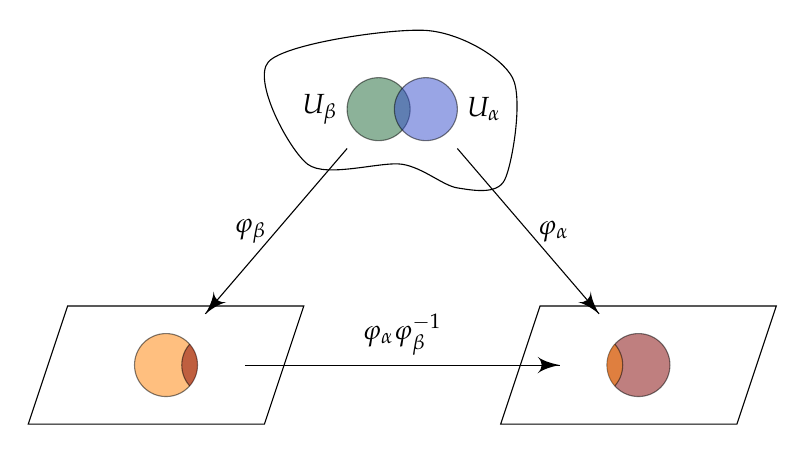
\begin{tikzpicture}
    \draw plot [smooth cycle] coordinates {(-1.2, -0.7) (0, -0.7) (0.7, -1) (1.3, -0.9) (1.4, 0.4) (0.3, 1) (-1.7, 0.6)};

    \draw (-0.3, 0) [fill=mgreen, opacity=0.5] circle [radius=0.4];
    \draw (0.3, 0) [fill=mblue, opacity=0.5] circle [radius=0.4];

    \node [left] at (-0.7, 0) {$U_\beta$};
    \node [right] at (0.7, 0) {$U_\alpha$};

    \begin{scope}[shift={(-4.75, -4)}]
      \draw (0, 0) -- (3, 0) -- (3.5, 1.5) -- (0.5, 1.5) -- cycle;

      \draw (1.75, 0.75) [fill=morange, opacity=0.5] circle [radius=0.4];
      \begin{scope}
        \clip (1.75, 0.75) circle [radius=0.4];
        \draw (2.35, 0.75) [fill=mred, opacity=0.5] circle [radius=0.4];
      \end{scope}
    \end{scope}

    \draw [->] (-0.7, -0.5) -- (-2.5, -2.6) node [pos=0.5, left] {$\varphi_\beta$};
    \draw [->] (0.7, -0.5) -- (2.5, -2.6) node [pos=0.5, right] {$\varphi_\alpha$};

    \begin{scope}[shift={(1.25, -4)}]
      \draw (0, 0) -- (3, 0) -- (3.5, 1.5) -- (0.5, 1.5) -- cycle;

      \draw (1.75, 0.75) [fill=mred, opacity=0.5] circle [radius=0.4];
      \begin{scope}
        \clip (1.75, 0.75) circle [radius=0.4];
        \draw (1.15, 0.75) [fill=morange, opacity=0.5] circle [radius=0.4];
      \end{scope}
    \end{scope}
    \draw [->] (-2, -3.25) -- (2, -3.25) node [pos=0.5, above] {$\varphi_\alpha \varphi_\beta^{-1}$};
  \end{tikzpicture}
\end{center}
$(U_\alpha, \varphi_\alpha)$  is called a \textbf{coordinate chart} and $\{(U_\alpha, \varphi_\alpha)\}_\alpha$ is called an \textbf{atlas}.  We can write
  \[
    \varphi_\alpha = (x^1, \cdots, x^n)
  \]
  where each $x_i: U_\alpha \to \R$. We call these the \textbf{local coordinates}. 

An important point of the definition of a smooth manifold is the following.  If $(U_\alpha, \varphi_\alpha)$ and $(U_\beta, \varphi_\beta)$ are charts in some atlas, and $f: M \to \R$, then $f \circ \varphi_\alpha^{-1}$ is smooth at $\varphi_\alpha(p)$ if and only if $f \circ \varphi_\beta^{-1}$ is smooth at $\varphi_\beta (p)$ for all $p \in U_\alpha \cap U_\beta$.


\begin{example}
  Consider the sphere
  \[
    S^n = \{x=(x_0, \cdots, x_n)\in \R^{n+1}: \sum x_i^2 = 1\} .
  \]
  We define an atlas as follows. We define an open covering
  \[
    U^+ = S^n \backslash \{\textrm{south pole}\},\quad U^- = S^2 \backslash \{\textrm{north pole}\}~.
  \]
  where the south pole is $x_0=-1$ and the north pole is $x_0=1$, and continuous maps
  \begin{align*}
&    \varphi^+: U^+ \to \R^n; (x_0, \cdots, x_n) \mapsto \frac{1}{1+x_0}(x_1, \cdots, x_n)\\
  &  \varphi^-: U^- \to \R^n; (x_0, \cdots, x_n) \mapsto \frac{1}{1-x_0}(x_1, \cdots, x_n)\\
  \end{align*}
Then, their inverse maps are
  \begin{align*}
(\varphi^\pm)^{-1}:\R^n\to U^\pm;(y_1,\dots,y_n)\mapsto \frac{1}{1+|y|^2}(\pm(1-|y|^2),y_1,\dots,y_n)~.
  \end{align*}
The transformation map
$$
\varphi^+ \cdots(\varphi^-)^{-1}(y)=\frac{y}{|y|}    \quad \varphi^- \cdots(\varphi^+)^{-1}(y)=\frac{y}{|y|} 
$$
\end{example}


Let $M$ and $N$  be smooth manifolds, and let $\{(U_\alpha, \varphi_\alpha)\}_\alpha$ and $\{(V_\beta, \psi_\beta)\}_\beta$ be their  atlas. We usually consider smooth maps between manifolds. 

\begin{defn}[Smooth map]\index{smooth map}
  A map $f: M \to N$ is \textbf{smooth} if, for a chart $(U_\alpha, \varphi_\alpha)$ of $p\in M$ and $(V_\beta, \psi_\beta)$ of $f(p)\in N$,  $ \psi_\beta \circ f \circ ( \varphi_\alpha)^{-1}: \varphi(U_\alpha \cap f^{-1} (V_\beta)) \to \xi(V_\beta )$ is smooth.


If it has smooth inverse, it is called \term{diffeomorphism}.

\end{defn}
\begin{center}
  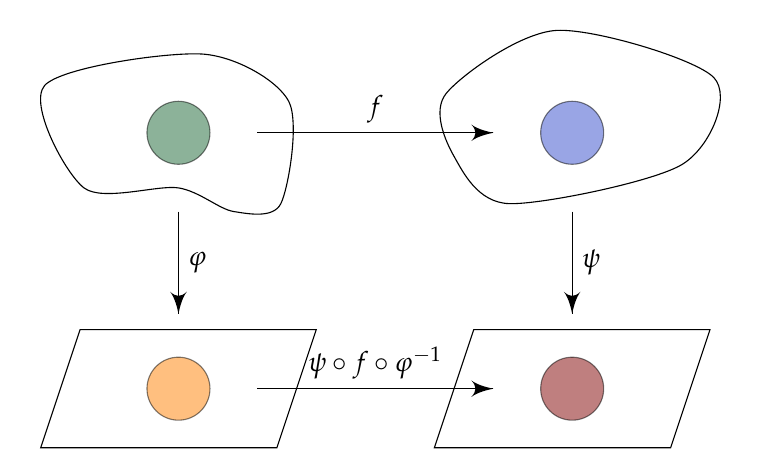
\begin{tikzpicture}
    \draw plot [smooth cycle] coordinates {(-1.2, -0.7) (0, -0.7) (0.7, -1) (1.3, -0.9) (1.4, 0.4) (0.3, 1) (-1.7, 0.6)};

    \draw [fill=mgreen, opacity=0.5] circle [radius=0.4];

    \begin{scope}[shift={(-1.75, -4)}]
      \draw (0, 0) -- (3, 0) -- (3.5, 1.5) -- (0.5, 1.5) -- cycle;

      \draw (1.75, 0.75) [fill=morange, opacity=0.5] circle [radius=0.4];
    \end{scope}

    \draw [->] (0, -1) -- +(0, -1.3) node [pos=0.5, right] {$\varphi$};
    \begin{scope}[shift={(5, 0)}]
      \draw plot [smooth cycle] coordinates {(1.4, -0.4) (-0.8, -0.9) (-1.5, -0.3) (-1.6, 0.5) (-0.2, 1.3) (1.8, 0.7)};

      \draw [fill=mblue, opacity=0.5] circle [radius=0.4];

      \begin{scope}[shift={(-1.75, -4)}]
        \draw (0, 0) -- (3, 0) -- (3.5, 1.5) -- (0.5, 1.5) -- cycle;

        \draw (1.75, 0.75) [fill=mred, opacity=0.5] circle [radius=0.4];
      \end{scope}

      \draw [->] (0, -1) -- +(0, -1.3) node [pos=0.5, right] {$\psi$};
    \end{scope}

    \draw [->] (1, 0) -- (4, 0) node [above, pos=0.5] {$f$};

    \draw [->] (1, -3.25) -- (4, -3.25) node [above, pos=0.5] {$\psi \circ f \circ \varphi^{-1}$};
  \end{tikzpicture}
\end{center}
Equivalently, $f$ is smooth at $p$ if $\xi \circ f \circ \varphi^{-1}$ is smooth at $\varphi(p)$ for \textbf{any} such charts $(U, \varphi)$ and $(V, \xi)$.

\subsection{Tangent space}




\begin{defn}[Tangent vector]\index{Tangent vector}
A \textbf{tangent vector} $X_p$ at $p\in M$ is a map $X_p:C^\infty(M)\to \R$, which is subject to 
\begin{description}
\item{linearity} $X_p(\alpha f+\beta g)=\alpha X_p(f)+\beta X_p(g)$,  for  $\alpha,\beta \in \R$
\item{Leibniz rule} $X_p(fg)=f(p)X_p(g)+X_p(f) g(p)$
\end{description}
\end{defn}
Namely, a  \textbf{tangent vector} $X_p$  behaves like a differential operator on $C^\infty(M)$. Then, the set of tangent vectors at $p$ become a vector space
$$
(X_p+Y_p)(f)=X_p(f)+Y_p(f) \qquad (\alpha X_p)(f)=\alpha (X_p(f))~,
$$
and we call it the \textbf{tangent space} $T_pM$ at $p\in M$.


\begin{figure}[h]\centering
\includegraphics[width=8cm]{Tangentialvektor}
\end{figure}



There is another way to think about tangent vectors. Let us consider a \term{curve}, which is a smooth map $\gamma:I \to M$ with $\gamma(0)=p$ where $I$ is a non-empty open interval. Two curves $\gamma_1,\gamma_2$ are \textbf{tangent} at $p$ if 
$$
\gamma_1(0)=p=\gamma_2(0)~, \qquad  \frac{d}{dt}\varphi(\gamma_1(t))\Big|_{t=0}= \frac{d}{dt}\varphi(\gamma_2(t))\Big|_{t=0}
$$
where $(U,\varphi)$ is a chart around $p$. We write  two tangent curves $\gamma_1\sim \gamma_2$, which forms an equivalence class.
\begin{figure}[h]\centering
\includegraphics[width=5cm]{tangent-curve}
\end{figure}
For ${}^\forall f\in C^\infty(M)$, We can then take the derivative of $f$ along $\gamma$ 
\[
  X_p(f) = \left.\frac{\d}{\d t}\right|_{t = 0} f(\gamma(t))~.
\]
It is easy to see that $X_p$ satisfies the definition of a tangent vector. So we can provide the definition of the tangent space at $p$ as
$$
T_pM=\{ \gamma:I\to M | \gamma(0)=p\}/\sim
$$
Given a local coordinate $\varphi=( x^1, \cdots, x^n)$, the tangent vector along a curve $\gamma$ can be written as
$$
X_p=\sum_{i=1}^n X_p^i\frac{\partial}{\partial x^i}\Big|_p   \quad \textrm{where} \quad X_p^i=\frac{d}{dt}x^i(\gamma(t))\Big|_{t=0}~.
$$
Therefore, $(\frac{\partial}{\partial x^1}\Big|_p,\cdots,\frac{\partial}{\partial x^n}\Big|_p)$ can be considered as a basis of $T_pM$.
Suppose we also have coordinates $y_1, \cdots, y_n$ near $p$ given by some other chart. Then, we can write 
\[
  \left.\frac{\partial}{\partial y_i}\right|_p = \sum_{j = 1}^n \frac{\partial x_j}{\partial y_i}(p)\left.\frac{\partial}{\partial x_j}\right|_p~,
\]
where $ \frac{\partial x_j}{\partial y_i}(p)$ is called \term{Jacobian} at $p$.


\subsection{Tangent bundles}
Let us consider a collection of tangent spaces over every point $p$ on $M$
\[
  TM = \bigcup_{p \in M} T_p M=\{(p,X_p)|p\in M ~, X_p\in T_pM\}~.
\]
into a manifold. There is then a natural map $\pi: TM \to M$ sending $X_p \in T_pM$ to $p$ for each $p \in M$, and this is smooth. 

We can consider $TM$ as a manifold of dimension $2 \dim M$, which is called the \textbf{tangent bundle} of $M$.
  Let $x^1, \cdots, x^n$ be coordinates on a chart $(U, \varphi)$. Then for any $p \in U$ and $X_p \in T_p M$, there are some $\alpha^1, \cdots, \alpha^n \in \R$ such that
  \[
    X^p = \sum_{i = 1}^n \alpha^i \left.\frac{\partial}{\partial x^i}\right|^{p}.
  \]
  This gives a bijection
  \begin{align*}
    \pi^{-1}(U) &\to \varphi(U) \times \R^n\\
    X^p &\mapsto (x^1(p), \cdots, x^n(p), \alpha^1, \cdots, \alpha^n),
  \end{align*}
  If $(V, \xi)$ is another chart on $M$ with coordinates $y^1, \cdots, y^n$, then
  \[
    \left.\frac{\partial}{\partial x^i}\right|^p = \sum_{j = 1}^n \frac{\partial y^j}{\partial x^i}(p) \left.\frac{\partial}{\partial y^j}\right|^p.
  \]
  So we have $\tilde{\xi} \circ \tilde{\varphi}^{-1}: \varphi(U \cap V) \times \R^n \to \xi(U \cap V) \times \R^n$ given by
  \[
    \tilde{\xi} \circ \tilde{\varphi}^{-1} (x^1, \cdots, x^n, \alpha^1, \cdots, \alpha^n) = \left(y^1, \cdots, y^n, \sum_{i = 1}^n \alpha^i \frac{\partial y^{1}}{\partial x^i}, \cdots, \sum_{i = 1}^n \alpha^i \frac{\partial y^n}{\partial x^i}\right),
  \]
  and is smooth (and in fact fiberwise linear).



\subsection{Vector fields}


A smooth map $X:M\to TM$ is called a \textbf{section} if $X\cdot \pi=id_M$. Since it is actually a smooth assignment $X:p \mapsto X(p)$, it is called a \term{vector field}. 

\begin{example}
Let $S^n\subset \R^{n+1}$ be an $n$-sphere. We have a vector field 
$$
Y=\sum Y^i\frac{\partial}{\partial x^i}
$$
where 
$$
Y^i=\left\{ \begin{array}{ll} (-x^1,x^0,-x^3,x^2,\cdots,-x^{2k},x^{2k-1}) & n=2k+1\\ (-x^1,x^0,-x^3,x^2,\cdots,-x^{2k},x^{2k-1},0) & n=2k+2\end{array}\right.~.
$$
\end{example}

\begin{figure}[h]\centering
\includegraphics[width=5cm]{vector-field}
\end{figure}

We write a set of vector fields by $\mathfrak{X}(M)=\Gamma(TM)$. In fact, a vector field $X\in \mathfrak{X}(M)$ is a map $C^\infty(M)\to C^\infty(M)$, which satisfies 
 \begin{align}\nonumber
& X(\alpha f+\beta g)=\alpha X(f)+\beta X(g),  \quad \textrm{for} \quad \alpha,\beta \in \R\cr
&X(fg)=fX(g)+X(f) g~.
\end{align}
Let $X, Y \in \mathfrak{X}(M)$, and $f \in C^\infty(M)$.   Then we have $X + Y, fX \in \mathfrak{X}(M)$. Therefore, $\mathfrak{X}(M)$ is a $C^\infty(M)$-module.



Note that the product of two vector fields $X,Y\in \mathfrak{X}(M)$ is not a vector field:
\begin{align*}
  XY(fg) &= X(Y(fg)) \\
  &= X(fY(g) + gY(f)) \\
  &= X(f) Y(g) + fXY(g) + X(g) Y(f) + g XY(f).
\end{align*}
 However, that $XY - YX$ is a vector field and we denote it as $[X, Y]$, called the \term{Lie bracket}. In fact, $\mathfrak{X}(M)$ with Lie bracket satisfies
  \begin{enumerate}
    \item $[\ph, \ph]$ is bilinear.
    \item $[\ph, \ph]$ is antisymmetric, i.e.\ $[X, Y] = -[Y, X]$.
    \item The \term{Jacobi identity} holds
      \[
        [X, [Y, Z]] + [Y, [Z, X]] + [Z, [X, Y]] = 0.
      \]
  \end{enumerate}



\subsection{Flows}
 An \term{integral curve} of $X \in \mathfrak{X}(M)$ is a smooth $\gamma: I \to M$ such that $I$ is an open interval in $\R$ and
  \[
    \dot{\gamma}(t) = X_{\gamma(t)}.
  \]

\begin{example}
A vector field $X=\alpha \frac{\partial }{\partial x} +\beta  \frac{\partial }{\partial y}$ in $\R^2$. Then, the integral curve is a translation
$$
\gamma_t(x,y)=(x+t\alpha,y+t\beta)~.
$$  
\end{example}



\begin{thm}[Existence of integral curves]
  Let $X \in \mathfrak{X}(M)$ and $p \in M$. Then there exists some open interval $I \subseteq \R$ with $0 \in I$ and an integral curve $\gamma: I \to M$ for $X$ with $\gamma(0) = p$.

  Moreover, if $\tilde{\gamma}: \tilde{I} \to M$ is another integral curve for $X$, and $\tilde{\gamma}(0) = p$, then $\tilde{\gamma} = \gamma$ on $I \cap \tilde{I}$.
\end{thm}

Let $M$ be a a compact manifold. A smooth map  
$$
\gamma:\R\times M \to M ; (t,p)\mapsto \gamma_t(p)
$$
is called \textbf{flow} (or one-parameter group of diffeomorphisms) generated by a vector $X$ if 
$$
\gamma_{t+s}(p)=\gamma_t(\gamma_s(p))~, \quad \frac{d\gamma_t(p)}{dt}=X_{\gamma_t(p)}~.
$$




\subsection{Orientation}
Suppose we have picked two ordered bases $(e_1, \cdots, e_n)$ and $(\tilde{e}_1, \cdots, \tilde{e}_n)$ of $T_pM$.  Then, we define an equivalence class  $(e_1, \cdots, e_n)\sim (\tilde{e}_1, \cdots, \tilde{e}_n)$ iff
\[
  e_i = \sum_j B_{ij} \tilde{e}_j \qquad  \det B > 0~.
\]
We call the two ordered bases have the \term{same orientation} if they are the same equivalence class. Therefore, for $p\in M$, we can assign an orientation $\mathcal{O}_p$. If we can give continuous assignment $p\mapsto \mathcal{O}_p$, then $M$ is called \term{orientable}.



A smooth manifold $M$ is orientable iff there exists an atlas  $\{(U_\alpha, \varphi_\alpha)\}_\alpha$ of $M$ such that the determinant of the Jacobian is positive on any $U_\alpha\cap  U_\beta$.


\begin{figure}[h]\centering
\includegraphics[width=4.5cm]{orientation-strip}
\caption{The M\"obius strip is not orientable.}
\end{figure}




\section{Lecture 3: \cite{Nakahara} \S 5.4, 5.5}


\subsection{Cotangent bundles}


Given a vector space $V$, one can take its dual space 
$$
V^*=\{f:V\to\R | f(\alpha_1 v_1+\alpha_2 v_2)=\alpha_1 f(v_1)+\alpha_2 f(v_2)\}
$$
The dual space $V^*$ is also a vector space: $\beta_1 f_1 +\beta_2 f_2 \in V^*$ for $f_1,f_2\in V^*$ and $\beta_1,\beta_2\in \R$.
The dual vector space $T_p^*M$ of the tangent space $T_pM$ is called the \term{cotangent space}. In fact, given $f\in C^\infty(M)$, we can define its differential $df_p$ at $p$
$$
df_p:T_pM\to \R;X_p \mapsto X_p(f)~.
$$
For a local coordinate $(U,\varphi=(x^1,\cdots,x_n))$, we have seen that $(\frac{\partial}{\partial x^1}\Big|_p,\cdots,\frac{\partial}{\partial x^n}\Big|_p)$ is  a basis of $T_pM$. On the other hand, we can take $(dx^1|_p,\cdots,dx^n|_p)$ as a basis of $T^*_pM$ so that $$dx^i|_p(\frac{\partial}{\partial x^j}\Big|_p)=\delta^j_i~.$$
Therefore, in this basis, we can write
$$
df_p=\sum_{i=1}^n\frac{\partial f}{\partial x^i}(p) dx^i|_p
$$
Like the tangent bundle, we can consider a collection of the cotangent spaces
$$
T^*M=\cup_{p\in M} T^*_pM
$$
which has a manifold structure. We call $T^*M$ the \term{cotangent bundle} of $M$. Moreover, the section of the cotangent bundle is called one-form, and we denote the set of one-form by $\Omega^1(M)=\Gamma(T^*M)$.
  For example, if $f$ is a smooth function on $M$, then $d f \in \Omega^1(M)$, which can take a paring with ${}^\forall X \in \mathfrak{X}(M)$
  \[
    d f(X) = X(f)~.
  \]
 


\subsubsection{push-forward and pull-back}

Let $f: M \to N$  be a smooth map between smooth manifolds $M$ and $N$. It induces a push-forward of tangent vectors
$$
f_*:T_pM\to T_{f(p)}N
$$
which is defined by
$$
f_*(X_p)(g)=X_p(g\circ f)
$$
for $g\in C^\infty(N)$. 
\begin{figure}[h]\centering
\includegraphics{fig_tangent_map}
\end{figure}

On the other hand, it induces pull-back of the cotangent space
$$
f^*: T^*_{f(p)}N\to T^*_pM
$$
which is defined by
$$
\langle f^*\omega_{f(p)}, X_p\rangle=\langle\omega_{f(p)},f_*X_p\rangle
$$
for $\omega_{f(p)}\in T_{f(p)}N$ where $\langle \cdot ,\cdot \rangle$ is a natural paring between the tangent and cotangent space. 






\subsection{Differential forms}
In general, given a vector space $V$ and its dual vector space $V^*$, one can consider $k$-forms, which are alternating $k$-linear maps $\wedge^k V^*$.
Let us start with a product of 1-forms. If $\alpha_a$ are 1-forms (i.e., $\alpha_a \in V^*$), their wedge products are defined by
$$\alpha_1\wedge\alpha_2\wedge\cdots\wedge\alpha_k(v_1,v_2,\cdots,v_k)=\det(\alpha_a(v_b))~.$$ 
More generally, if $\alpha$ is a $k$-form and $\beta$ is an $\ell$-form,
$$(\alpha\wedge \beta)(v_1, \cdots, v_{k+\ell}) = \frac{1}{(k+\ell)!} \sum_{\sigma\in S_{k+\ell}} \textrm{sign} \sigma 
~  \alpha(v_{\sigma(1)} , \cdots, v_{\sigma(k)} )\beta(v_{\sigma(k+1)} , \cdots, v_{\sigma(k+l)} )~.$$ k!l!
We can choose a basis of the space of $k$-forms, $\wedge^k V^*$, as $e_{i_1}\wedge\cdots\wedge e_{i_k}$.
 Any $k$-form $\alpha$ can be expanded as
$$\alpha= \frac{1}{ k!}\sum_{I} \alpha_{i_1,\cdots,i_k}e_{i_1}\wedge\cdots\wedge e_{i_k}.$$



Therefore, one can consider the $k$-th wedge product $\wedge^k T_p^*M$ of the cotangent space $T^*_pM$ and its bundle $\wedge^k T^*M$.   We write the set of sections as
  \[
    \Omega^k (M) = \Gamma(\Lambda^k T^*M) = \{\text{$k$-forms on $M$}\}.
  \]
  An element of $\Omega^k(M)$ is known as a \term{differential $k$-form}.
  In particular, we have
  \[
    \Omega^0(M) = C^\infty(M).
  \]
In local coordinates $x^1, \cdots, x^n$ on $U$ we can write $\omega \in \Omega^k(M)$ as
\[
  \omega = \sum_{i_1 < \ldots < i_p} \omega_{i_1, \ldots, i_p} d x^{i_1} \wedge \cdots \wedge d x^{i_p}
\]
for some smooth functions $\omega_{i_1, \ldots, i_p}$.


Moreover, there exists a unique linear map called \term{exterior derivative}
  \[
    d : \Omega^k(M) \to \Omega^{k + 1}(M)~,
  \]
  such that
  \begin{enumerate}
    \item On $\Omega^0(M)$ this is as previously defined, i.e.
      \[
        d f (X) = X(f)\text{ for all }X \in \mathfrak{X}(M).
      \]
    \item We have
      \[
        d \circ d = 0: \Omega^k(M) \to \Omega^{k + 2}(M).
      \]
    \item It satisfies the \term{Leibniz rule}
      \[
        d (\omega \wedge \sigma) = d \omega \wedge \sigma + (-1)^k \omega \wedge d \sigma.
      \]
  \end{enumerate}



In term of local coordinates $x^1, \cdots, x^n$, we can define the exterior derivative as
  \[
    d\left(\sum_{i_1 < \ldots < i_p} \omega_{i_1, \ldots, i_p}\;d x^{i_1} \wedge \cdots \wedge d x^{i_p}\right) = \sum d \omega_{i_1, \ldots, i_p}\wedge d x^{i_1} \wedge \cdots \wedge d x^{i_p}~.
  \]
  
  
  
  Let $f: M \to N$  be a smooth map between smooth manifolds $M$ and $N$. The pull-back of differential forms associated to $f$ can be defined as
  \[
    (f^*\omega|_p)(v_1, \cdots, v_k) = \omega|_{f(p)} (df|_p(v_1), \cdots, df|_p(v_k)).
  \]
  for $\omega\in \Omega^k(N)$ and  $v_1, \cdots, v_k \in T_p M$. Note that the pull-back $f^*$ has the following property
  \begin{enumerate}
    \item $f^*:\Omega^k(N) \to \Omega^k(M)$ is a linear map.
    \item $f^*(\omega \wedge \sigma) = f^*\omega \wedge f^*\omega$.
    \item If $g :N\to L$ is a smooth map between two manifolds $N$ and $L$, then $(g \circ f)^* = f^* \circ g^*$.
    \item It commutes with exterior derivative: $df^* = f^* d$.
  \end{enumerate}
  
  \subsection{Integrals of differential forms}
  
    Let $M$ be $n$-dimensional orientable smooth manifold and $\omega\in \Omega^n(M)$.  We would like to define the integral of $\omega$ over $M$. To this end, we define a partition of unity.

  
  \begin{defn}[Partition of unity]\index{partition of unity}
  Let $\{U_\alpha\}$ be a locally-finite open cover of a manifold $M$. A \term{partition of unity} associated to $\{U_\alpha\}$ is a collection $\chi_\alpha \in C^\infty(M, \R)$ such that
  \begin{enumerate}
    \item $0 \leq \chi_\alpha \leq 1$
    \item $\supp(\chi_\alpha) \subseteq U_\alpha$
    \item $\sum_\alpha \chi_\alpha = 1$.
  \end{enumerate}
\end{defn}

If we use local coordinate $(x^1,\cdots,x^n)$ on a chart $U_\alpha$, we can write
$$
\chi_\alpha \omega=f_\alpha(x) x^1\wedge\cdots\wedge x^n~.
$$
Therefore, we define its integral
$$
\int_M \chi_\alpha \omega=\int \cdots \int f_\alpha(x) x^1\cdots x^n~.
$$
Then, we can define
$$
\int_M\omega=\sum_\alpha\int_M \chi_\alpha \omega~.
$$
One can show that this is independent of choice of a locally-finite open covering $\{U_\alpha\}$  and a partition of unity on $\{U_\alpha\}$ .
  
  \begin{thm}[Stokes' theorem]\index{Stokes' theorem}
  Let $M$ be an oriented manifold with boundary of dimension $n$. Then if $\omega \in \Omega^{n - 1}(M)$ has compact support, then
  \[
    \int_M d \omega = \int_{\partial M}\omega.
  \]
  In particular, if $M$ has no boundary, then
  \[
    \int_M d \omega = 0~.
  \]
\end{thm}




\section{Lecture 4: \cite{Nakahara} \S 6.2, 6.3, 6.4, 7.1 and 7.9}


\subsection{de Rham cohomology}

Given a differential operator 
$$
d:\Omega^k(M)\to\Omega^{k+1}(M)~,
$$
$\omega\in\Omega^k(M)$ is called a \textbf{closed form} if $d\omega=0$, and   an \textbf{exact form} if there exists $(k-1)$-form such that $\omega=d\eta$. Let us denote the set of all closed $k$-forms on $M$ by $Z^k(M)$ and the set of all exact $k$-forms by $B^k(M)$. 
\begin{align}
Z^k(M)&=\textrm{Ker}(d:\Omega^k(M)\to\Omega^{k+1}(M))\cr
B^k(M)&=\textrm{Im}(d:\Omega^{k-1}(M)\to\Omega^{k}(M))\nonumber
\end{align}
The de Rham cohomology group of $M$ is defined as the quotient space 
$$
H^k_{dR}(M)=Z^k(M)/B^k(M)
$$
In other words, the de Rham cohomology group of $M$ is the cohomology of de Rahm complex
$$
0\to \Omega^0(M) \xrightarrow{d}\Omega^1(M) \xrightarrow{d}\cdots  \xrightarrow{d} \Omega^n(M)\to0
$$

\begin{lem}[Poincar\'e Lemma]
The de Rham cohomology of $\bR^n$ is trivial. That is, 
$$
H^k(\bR^n)=\left\{\begin{array}{l} \bR \quad k=0 \\ 0 ~ \quad  k\neq 0\end{array}\right.
$$
\end{lem}
This also holds when $M$ is contractible, namely when one can smoothly shrink $M$ to a point. This is not true on a general manifold. However, it is true on each coordinate chart. The issue is how these charts are patched together globally.


\subsection{Metric}


A metric $g$ on $M$ is symmetric and non-degenerate bilinear form
$$g_p:T_p M\times T_p M\to \bR$$
in such a way that $g_p$ is smooth with respect to $p$. Its components are given by $g_{ij}=g(\partial_i,\partial_j)$. If $g_{ij}$ is positive definite, $(M,g)$ is called a Riemannian manifold. In a chart $U,(x^1\cdots,x^n)$, it can be written locally as
$$
ds^2= g_{ij}(x)dx^i\otimes dx^j~.
$$
On an arbitrary smooth manifold, one can show there exists a Riemannian metric by using a partition of unity.
On a Riemannian manifold, one can introduce the notion of the length of a tangent vector $v\in T_pM$
$$
||v||=\sqrt{g(v,v)}~.
$$
For a curve $c:[a,b]\to M$, the length $L(c)$ of curve can be defined by
$$
L(c)=\int_{a}^b ||\dot c(t)||dt=\int_a^b \sqrt{g_{ij}\frac{dx^i}{dt}\frac{dx^j}{dt}}
$$

For a smooth map $f:M\to N$, the metric $g$ on a smooth manifold $N$ can be pull-back to the metric $f^*g$ on a smooth manifold $M$ in such a way that for $v,w\in T_pM$
$$
f^*g(v,w)=g(f_*v,f_*w)~.
$$

\begin{defn}[Isometry]\index{isometry}
  Let $(M, g)$ and $(N, h)$ be Riemannian manifolds. We say $f: M \to N$ is an \emph{isometry} if it is a diffeomorphism and $f^*h = g$. In other words, for any $p \in M$ and $u, v \in T_p M$, we need
  \[
    h\big(f_* u, f_* v\big) = g(u, v).
  \]
\end{defn}
In fact, given isometries $f_1,f_2$, its product $f_1\circ f_2$ is also an isometry so that  the set of isometries forms a group, called the \textbf{isometry group}. 
\vspace{.5cm}

For instance, any reflection, translation and rotation is a global isometry on Euclidean spaces. The isometry group $E(n)$ of $\bR^n$ is the Euclidian group, and  therefore it has as subgroups the translational group $T(n)$, and the orthogonal group $O(n)$. Any element of $E(n)$ is a translation followed by an orthogonal transformation (the linear part of the isometry), in a unique way:
$$
x \mapsto A (x + b)
$$
where $A\in O(n)$ is an orthogonal matrix.

\vspace{.5cm}

Using a metric $g$, one have an isomorphism between the vector field and one form 
$$
\hat g: \mathfrak{X}(M) \cong \Omega^1(M)
$$
in such a way that for vector fields $v,w\in  \mathfrak{X}(M)$ on $M$,
$$
\hat g(v)(w)=g(v,w)
$$
By using the isomorphism $T_pM\cong T^*_pM$, we can introduce an inner product on $T^*_pM$.


\subsection{Vielbeins, volume form, Hodge $\ast$ operator}

For simplicity, we will assume that the metric $g_{ij}$ is positive definite. For a metric with more general signature, we just have to introduce appropriate sign factors to some of the formulae below.
Since the metric $g_{ij}$ is symmetric, we can find a basis $\{e^a_i \}$ $(a=1,\cdots ,n)$ so that
$$
g_{ij} =
\sum^n_{a=1} e^a_ie^a_j~. 
$$
This basis is called \textbf{the orthonormal frame}. For a given metric, an orthonormal frame is defined modulo $O(n)$.


This can be done at each point $p$ on $M$. $e^a$'s are called \textbf{vielbeins} where viel means many in German, and bein is a leg. (In 4 dimensions, they are also called vierbeins or tetrads. In dimensions other than 4, words like f\"unfbein, etc. have been used. Vielbein covers all dimensions.)
Using the vierbeins, the volume form vol is defined by 
$$\textrm{vol} = e^1 \wedge e^2 \wedge \cdots \wedge e^n~.$$
Note that it may not be possible to define vol globally on $M$ since it is invariant under $SO(n)$ but not under $O(n)$. It may not be possible to choose a sign factor for vol (associated to $\bZ_2 = O(n)/SO(n)$) consistently over $M$. The volume form is well-defined if and only if $M$ is orientable.


Using coordinates, we can express the volume form as
$$\textrm{vol} = \sqrt{g}dx_1 \wedge dx_2 \wedge \cdots \wedge dx_n~,$$
where $g = \det g$ (we are assuming that the metric is positive definite). There is an isomorphism 
$$
\ast : \Omega^k(M)\to \Omega^{n-k}(M)
$$
is defined by
$$
\ast(e^1\wedge \cdots \wedge e^k)=e^{k+1}\wedge \cdots \wedge e^n
$$
For a $k$-form $\omega$, the \textbf{Hodge $\ast$ operator} is defined as 
$$
(\ast \omega)_{i_{k+1}\cdots i_n}=\frac{1}{k!} \frac{\epsilon^{j_1\cdots j_kj_{k+1}\cdots j_n}}{\sqrt{g}}\omega_{j_1\cdots j_k}g_{j_{k+1}i_{k+1}}\cdots g_{j_ni_n}~.
$$
Here I used the totally anti-symmetric tensor $\epsilon_{i_1\cdots i_n}$ and $\epsilon^{i_1\cdots i_n}$ normalized as 
$$
\epsilon_{12\cdots n}=\epsilon^{12\cdots n}=1
$$
The important point is that the Hodge star depends on the metric $g$.    Under coordinate transformations,  $\epsilon_{i_1\cdots i_n}$  does not transform as a tensor. However, we can remedy this by multiplying 
$\sqrt{g}$ to make it into the volume form. The volume form transforms as a tensor if coordinate transformations preserve the orientation. If we change the orientation, we get an extra $(-1)$. 

\subsection{Adjoint operator} 
The adjoint operator $\delta$ on $\Omega^k$ of the exterior differential $d$ is defined by
$$\delta\omega = (-1)^{nk+n+1} \ast d \ast \omega~.$$
We have commutative diagram
$$
\begin{tikzcd}
\Omega^k(M) \arrow[r, "\ast"] \arrow[d, "\delta"]
& \Omega^{n-k}(M) \arrow[d, "d" ] \\
\Omega^{k-1}(M)\arrow[r,  "(-1)^k\ast"]
& \Omega^{n-k+1}(M)
\end{tikzcd}
$$
We can easily verify the following properties,
$$\delta^2 =0~,\quad \ast\delta d=d\delta\ast~,\quad d\ast \delta=\delta 
\ast d=0~.$$
It is an adjoint operator in the sense that 
$$
(d\omega,\eta)=(\omega,\delta\eta)~.
$$
where we assume that $M$ is an oriented, compact, closed manifold.
where the inner product on $\Omega^k(M)$ is defined by
$$
(\rho,\sigma)=\int_M \rho\wedge \ast \sigma =\int_M\sigma\wedge \ast \rho
$$

On a Riemannian manifold $M$, an operator defined by
$$\Delta= \delta d + d\delta : \Omega^k(M) \to \Omega^k(M)~$$
is called \textbf{Laplace-Beltrami operator}. A form $\omega\in\Omega^*(M)$ such that $\Delta\omega=0$ is called a \textbf{harmonic form}. In particular, a function $f$ such that $\Delta f=0$ is called a \textbf{harmonic function}.
One can show that a necessary and sufficient condition of harmonic form: $\Delta\omega=0$ iff $d\omega=0=\delta\omega$.

\subsection{Hodge theorem and Hodge decomposition}
Let us denote the set of all harmonic $k$-forms on $M$
$$
\bH^k(M)=\{\omega\in\Omega^k(M)|\Delta\omega=0\}~.
$$

\begin{thm}[Hodge theorem]
On an oriented compact Riemanninan manifold,  the natural map $\bH^k(M)\to H^k_{dR}(M)$ is isomorphism. 
\end{thm}


\begin{thm}[Hodge decomposition]
For an oriented compact Riemanninan manifold, we have the orthogonal decomposition
$$
\Omega^k(M)=\bH^k(M)\oplus d\Omega^{k-1}(M)\oplus \delta\Omega^{k+1}(M)
$$ 
\end{thm}







Applications of the Hodge theorem is as follows.








\begin{thm}[Poincare duality]
For an connected, oriented, compact $n$-dimensional Riemanninan manifold, the bilinear map 
$$
H_{dR}^k(M)\times H_{dR}^{n-k}(M)\to \bR; ~(\omega,\eta)\mapsto \int_M\omega\wedge \eta
$$
is  non-degenerate and hence induces an isomorphism
$$
H_{dR}^{n-k}(M) \cong  H_{dR}^k(M)^*
$$
\end{thm}


The Hodge theorem tells us that $\omega\in H^*k(M)$ is a harmonic form. Due to $d\ast =\ast d$, $\eta=\ast \omega$ is also a harmonic form. If $\omega\neq 0$, we have 
$$
\int_M\omega\wedge \eta=||\omega ||^2\neq0
$$




\section{Lecture 5: \cite{Nakahara} \S 7.2, 7.3, and 7.4}


\subsection{Covariant derivative and parallel transport}


Let $X$ and $Y$ be vector fields on $M$.
The symbol $\nabla_XY$ denotes the derivative of the vector field $Y$ along trajectories of the vector field $X$. In fact, it is a map
$$
\nabla:\frakX(M)\times \frakX(M)\to \frakX(M); (X,Y)\mapsto \nabla_XY
$$
which satisfies the following conditions
\begin{itemize}
\item $\nabla$ is linear in the first variable and additive in the second: $$\nabla_{fX+hY}Z\;=\;f\nabla_XZ+h\nabla_YZ$$
    $$\nabla_X(Y+Z)\;=\;\nabla_XY\,+\,\nabla_XZ$$ where $f,h\in \bC^\infty(M)$ are functions and $X,Y\in\frakX(M)$ are vector fields.
\item $\nabla$ obeys the Leibnitz rule in the second variable: $$\nabla_X(fY)\;=\;X(f)Y\,+\,f\nabla_XY~.$$
\end{itemize}
The operator $\nabla$ is called \textbf{covariant derivative} or the \textbf{connection}.



Let $(U,\{x^i\})$ be a chart on $M$.
Since $\nabla_{\partial/\partial{x^i}}\frac{\partial}{\partial{x}^j}$ is a vector field, it can be expressed as a linear combination of the coordinate fields:
\be
  \nabla_{\frac{\partial}{\partial x^j}} \frac{\partial}{\partial x^k} := \sum_{i = 1}^n \Gamma_{jk}^i \frac{\partial}{\partial x^i}.
\ee
These are called the \textbf{Christoffel symbols}.


Let $\gamma: I \to M$ be a curve on $M$ and we define
  \[
    J(\gamma) = \{\text{vector fields along $\gamma$}\}.
  \]
Then, given a  connection $\nabla$, we define the \textbf{covariant derivative} along $\gamma$, which is a map $\frac{D}{dt}: J(\gamma) \to J(\gamma)$ such that
  \begin{itemize}
    \item $\frac{D}{dt}(fX) = \dot{f} X + f \frac{D}{dt} X$ for all $f \in C^\infty(I)$
    \item If $X\in J(\gamma)$  is induced by  a vector field $\tilde X$  ($\tilde{X}|_{\gamma(t)} = X_t$ for all $t \in I$), then
      \[
        \frac{D}{dt}(X)\Big|_{t=0} = \nabla_{\dot{\gamma}(0)} \tilde{X}.
      \]
  \end{itemize}



Given a path $\gamma(t)$ (not necessarily a geodesic), a vector field $X$ is called \textbf{parallel}, or constant, along $\gamma$ if
\be
\frac{D}{dt}X\;=\;0.
\ee
In coordinates we can write
\be
\frac{d}{dt}=\frac{dx^i}{dt}\frac{\partial}{\partial{x}^i} \quad\quad X\;=\;X^j\frac{\partial}{\partial{x}^j}.
\ee
Using the axioms of covariant differentiation, we compute
\bea
\frac{D}{dt}X&=\nabla_{\frac{dx^i}{dt}\frac{\partial}{\partial{x}^i}}\left(X^j\frac{\partial}{\partial{x}^j}\right)\\
&=\frac{dx^i}{dt}\nabla_{\frac{\partial}{\partial{x}^i}}\left(X^j\frac{\partial}{\partial{x}^j}\right)\\
&=\frac{dx^i}{dt}\frac{\partial}{\partial{x}^i}\left(X^j\right)\frac{\partial}{\partial{x}^j}\,+\,\frac{dx^i}{dt}X^j\nabla_{\frac{\partial}{\partial{x}^i}}\frac{\partial}{\partial{x}^j}\\
&=\frac{d{X}^j}{dt}\frac{\partial}{\partial{x}^j}\,+\,\frac{dx^i}{dt}X^j\Gamma_{ij}^k\frac{\partial}{\partial{x}^k}\\
&=\left(\frac{d{X}^k}{dt}\,+\,\frac{dx^i}{dt}X^j\Gamma_{ij}^k\right)\frac{\partial}{\partial{x}^k}.
\eea
The Christoffel symbols $\Gamma_{ij}^k$, the path $\gamma$, and the derivatives $\frac{dx^i}{dt}$ are known.
Therefore the parallel transport equation is a system of $n$ first order linear differential equations:
\be
\frac{D}{dt}X\;=\;0 \quad\quad {\rm if}\;{\rm and}\;{\rm only}\;{\rm if} \quad\quad \frac{d{X}^k}{dt}\,+\,X^j\frac{dx^i}{dt}\Gamma_{ij}^k\;=\;0 \quad {\rm for} \; {\rm all} \; 1\,<\,k\,<\,n.
\ee
This means that given a single vector $X\in{T}_{\gamma(0)}M$, it can be \textbf{transported} along the curve $\gamma$ by solving this system of equations.







\subsection{Levi-Civita Connection}


Recall that in order to differentiate vectors, or even tensors on a manifold, we need a connection on the tangent bundle. There is a natural choice for the connection when a Riemannian metric is given.
\begin{defn}[Levi-Civita connection]\index{Levi-Civita connection}
  Let $(M, g)$ be a Riemannian manifold. The \emph{Levi-Civita connection} is the unique connection $\nabla$ on $M$ satisfying
  \begin{itemize}
    \item Compatibility with metric:\index{compatible connection}\index{connection!compatible with metric}
      \[
        Z g(X, Y) = g(\nabla_Z X, Y) + g(X, \nabla_Z Y),
      \]
    \item Symmetry/torsion-free:\index{symmetric connection}\index{torsion-free connection}\index{connection!symmetric}\index{connection!torsion-free}
      \[
        \nabla_X Y - \nabla_Y X = [X, Y].
      \]
  \end{itemize}
\end{defn}
With a bit more imagination on what the symbols mean, we can write the first property as
\[
  d (g(X, Y)) = g(\nabla X, Y) + g(X, \nabla Y),
\]
while the second property can be expressed in coordinate representation by
\[
  \Gamma_{jk}^i = \Gamma_{kj}^i~.
\]


On Riemannian manifold $(M,g)$, there exists a unique torsion-free  connection $\nabla$ compatible with $g$.
Using the metric compatibility condition
$$
\frac{\partial}{\partial x^i}g_{jk}=g\left(\nabla_{\frac{\partial}{\partial x^i}}\frac{\partial}{\partial x^j},\frac{\partial}{\partial x^k}\right)+g\left(\frac{\partial}{\partial x^j},\nabla_{\frac{\partial}{\partial x^i}}\frac{\partial}{\partial x^k}\right)
$$
Changing the index labels, we have the formula
\be
\Gamma_{ij}^k=\frac12\left(\frac{\partial{g}_{jl}}{\partial{x}^i}\,+\,\frac{\partial{g}_{il}}{\partial{x}^j}\,-\,\frac{\partial{g}_{ij}}{\partial{x}^l}\right)g^{lk}.
\ee


\begin{defn}[Geodesic]\index{geodesic}
  A curve $\gamma(t)$ on a Riemannian manifold $(M, g)$ is called a \emph{geodesic curve} if its tangent vectors are parallel transported along the curve itself with respect to the Levi-Civita connection:
  \[
    \frac{D \dot{\gamma}}{d t} = 0.
  \]
\end{defn}
In local coordinates, we write this condition as
  \[
  \ddot{x}_i + \Gamma^i_{jk}\dot{x}^j \dot{x}^k = 0.
  \]
A geodesic is uniquely specified by the initial conditions $p = x(0)$ and $a = \dot{x}(0)$.  This equation can be obtained as Euler-Lagrange equation of the action 
$$
S=\int \sqrt{g_{ij}\frac{dx^i}{dt}\frac{dx^j}{dt}}~,
$$
so, on a sufficiently small chart $U$, the curve is a shortest distant path with respect to the metric $g$.




\subsection{Riemann curvature}


We can consider doing some parallel transports on $S^n$ along the loop counterclockwise:
\begin{figure}[h]\centering
\includegraphics[width=5cm]{parallel}
\end{figure}
We see that after the parallel transport around the loop, we get a \emph{different} vector. The Riemann curvature is introduced to measure this difference.

The Riemann tensor is a map
$$
R:\frakX(M)\times \frakX(M)\times \frakX(M)\to \frakX(M);(X,\,Y,\,Z)\mapsto R(X,\,Y)\,Z
$$
where $R(X,\,Y)\,Z$ is defined as follows:
\be
R(X,\,Y)\,Z:=\nabla_X\nabla_YZ\;-\;\nabla_Y\nabla_XZ\;-\;\nabla_{[X,Y]}Z.
\ee
Note the obvious fact that $R$ is anti-symmetric in the first two variables:
\be
R(X,\,Y)\,Z\;=\;-R(Y,\,X)\,Z.
\ee
The Riemann tensor is also called the \textbf{curvature tensor}. 




On a chart, the Riemann tensor can be written in terms of the coordinate fields:
\be
R\left(\frac{\partial}{\partial{x}^i},\,\frac{\partial}{\partial{x}^j}\right)\,\frac{\partial}{\partial{x}^k}\;=\;{R^l{}_{kij}}\frac{\partial}{\partial{x}^l}.
\ee
In fact, we can show that the Riemann curvature can be expressed in terms of  Christoffel symbols 
\be
{R^l{}_{kij}}=\Gamma_{jk}^s\Gamma_{is}^l\;-\;\Gamma_{ik}^s\Gamma_{js}^l\;+\;\frac{\partial\Gamma_{jk}^l}{\partial{x}^i}\;-\;\frac{\partial\Gamma_{ik}^l}{\partial{x}^j}.
\ee


Essentially the Riemann tensor measures the {\bf failure of commutativity of two derivatives} when applied to vector fields.
\begin{figure}[h]\centering
\includegraphics[width=10cm]{parallelogram}
\end{figure}
Let us take infinitesimal parallelogram as in the figure. Then, the difference between the two vectors are indeed given by the Riemann curvature
$$
V_{C'}(r)-V_{C}(r)=V_0^j R^i_{jkl}\epsilon^k\delta^l
$$



Contracting the first and final indices of the Riemann tensor gives the \textbf{Ricci curvature tensor}
\be
R_{ij}={\textrm{Ric}}_{ij}:={R^s{}_{isj}}\;=\;R_{kijl}g^{kj}.
\ee
If there is a constant $\lambda$ such that $R_{ij}=\lambda g_{ij}$, $M,g$ is called a \textbf{Einstein manifold}.



Contracting again, we get the \textbf{scalar curvature}
\be
R:={\textrm{Ric}}_{ij}g^{ij}.
\ee
The scalar curvature is essentially the sum of all sectional curvatures at a point.


\subsubsection{Curvature dentities}

We can introduce the notation
\bea
R(X,\,Y,\,Z,\,W)&=\left<R(X,Y)Z,\,W\right>\\
R_{ijk\ell}&={R^s{}_{jk\ell}}g_{si}.
\eea
The Riemann tensor satisfy the following identity
\bea
&R(X,\,Y,\,Z,\,W)\;=\;-R(Y,\,X,\,Z,\,W)\\
&R(X,\,Y,\,Z,\,W)\;=\;-R(X,\,Y,\,W,\,Z)\\
&R(X,\,Y,\,Z,\,W)\;=\;R(Z,\,W,\,X,\,Y)\\
&R(X,\,Y)Z\,+\,R(Y,\,Z)X\,+\,R(Z,\,X)Y\;=\;0 \quad\quad\quad\quad {\rm (first}\,{\rm Bianchi}\,{\rm identity)}\\
&(\nabla_WR)(X,\,Y)Z\,+\,(\nabla_XR)(Y,\,W)Z\,+\,(\nabla_YR)(W,\,X)Z\;=\;0 \quad\quad {\rm (second}\,{\rm Bianchi}\,{\rm identity)}
\eea
In components, these read
\bea
&R_{ijkl}\;=\;-R_{ijlk}\\
&R_{ijkl}\;=\;-R_{jikl}\\
&R_{ijkl}\;=\;R_{klij}\\
&R_{lijk}\,+\,R_{ljki}\,+\,R_{lkij}\;=\;0\\
&R_{lijk,s}\,+\,R_{ljsk,i}\,+\,R_{lsik,j}\;=\;0.
\eea
Further identities can be derived by `mixing and matching' these identities.
For instance the second Bianchi identity is frequently presented
\be
R_{jkli,s}\,+\,R_{jlsi,k}\,+\,R_{jski,l}\;=\;0,
\ee
which can be derived from our second Bianchi identity and the rule $R_{ijkl}=R_{klij}$.

\subsection{Gauss-Bonnet theorem}

Let $(M,g)$ be a two-dimensional oriented closed manifold and vol is the volume form. Then Gauss curvature $\kappa$ is defined by
$$
\kappa:=-\frac{R_{1212}}{\det g} ~.
$$
Then, the Gauss-Bonnet theorem is 
$$
\frac{1}{2\pi} \int_M\kappa~ \textrm{vol}=\chi(M)~.
$$
It is remarkable in the sense that the integral in LHS is independent of choice of metric $g$ although the Gauss curvature $\kappa$  depends on the metric $g$. This formula connects differential geometry to topology. 

\subsection{Einstein equations}
The celebrated Einstein equations can be expressed
$$
R_{\mu \nu }-{\frac {1}{2}}Rg_{\mu \nu }+\Lambda g_{\mu \nu }={\frac {8\pi G}{c^{4}}}T_{\mu \nu }~,
$$
where $\Lambda$ is called the cosmological constant, $G$ is the Newton constant, $c$ is the speed of light and $T_{\mu\nu}$ is the stress-energy tensor. These are the Euler-Lagrange equations for the Einstein-Hilbert action
$$
S=\int \left[\frac {c^{4}}{16\pi G}\left(R-2\Lambda \right)+{\mathcal  {L}}_{{\mathrm  {M}}}\right]{\sqrt  {-g}}\,{\mathrm  {d}}^{4}x~.
$$



In this equation, a metric becomes dynamical variable and, roughly speaking, the curvature tensor of the spacetime is determined by the stress-energy tensor of matter. The equation is highly non-linear so that it can be solved analytically only in very special situations. The most of the cases requires  numerical simulations to solve the Einstein equations. Remarkably, this equation describes nature at terrestrial scale, and predicts the gravitational wave, which was detected by LIGO last year. (The No.1 candidate of Nobel physics prize this year!) It also describes the history of the universe \cite{Weinberg}.



\section{Lecture 6: \cite{Nakahara} \S 4}

\subsection{Homotopy}





In topology, we study spaces up to ``continuous deformation''. Famously, a coffee mug can be continuously deformed into a doughnut, and thus they are considered to be topologically the same. Now we also talk about maps between topological spaces. So a natural question is if it makes sense to talk about the continuous deformations of maps. It turns out we can, and the definition is sort-of the obvious one:

\begin{figure}[h]\centering
\includegraphics{homotopy}
\end{figure}


\begin{defn}[Homotopy]\index{homotopy}
  Let $X, Y$ be a topological space. A \textbf{homotopy} between $f_0, f_1: X \to Y$ is a map $F: [0, 1] \times X \to Y$ such that $F(0, x) = f_0(x)$ and $F(1, x) = f_1(x)$. If such an $F$ exists, we say $f_0$ is \textbf{homotopic} to $f_1$, and write $f_0 \simeq f_1$.
\end{defn}

	

\begin{figure}[h]\centering
\includegraphics{equiv-homotopy}
\end{figure}

As easily can ben seen from the figure above, homotopy $\simeq$ defines an equivalence relation on the set of maps from $X$ to $Y$.
In algebraic topology, we study quantities invariant under homotopies. 


\begin{defn}[Homotopy equivalence]\index{homotopy equivalence}
  A map $f: X \to Y$ is a \textbf{homotopy equivalence} if there is some $g: Y \to X$ such that $f \circ g \simeq \id_X$ and $g \circ f \simeq \id_Y$. We call $g$ the \textbf{homotopy inverse}\index{homotopy inverse} to $f$.
\end{defn}


  If $f_0 \simeq f_1: X \to Y$ and $g_0 \simeq g_1: Y \to Z$, then $g_0 \circ f_0 \simeq g_1 \circ f_1: X \to Z$.
  \[
    \begin{tikzcd}
      X \ar[r, bend left, "f_0"] \ar[r, bend right, "f_1"'] & Y \ar[r, bend left, "g_0"] \ar[r, bend right, "g_1"'] & Z
    \end{tikzcd}
  \]
Therefore, homotopy equivalence is an equivalence relation.

%\begin{example}[Stupid example]
%  If $f: X \to Y$ is a homeomorphism, then it is a homotopy equivalence --- we take the actual inverse for the homotopy inverse, since equal functions are homotopic.
%\end{example}

\begin{example}
  Let $i: \{0\} \to \R^n$ be the inclusion map. A homotopy equivalence can be constructed by
  $F: [0, 1] \to \R^n \to \R^n$ be
  \[
    F(t, \mathbf{v}) = t\mathbf{v}.
  \]
  We have $F(0, \mathbf{v}) = 0$ and $F(1, \mathbf{v}) = \mathbf{v}$.  From the point of view of homotopy, the point $\{0\}$ is equivalent to $\R^n$, so that dimension is irrelevant.
\end{example}


\begin{example}
  Let $S^n \subseteq \R^{n + 1}$ be the unit sphere, and $i: S^n \hookrightarrow \R^{n + 1} \setminus \{0\}$. We show that this is a homotopy equivalence. We define $r: \R^{n + 1} \setminus \{0\} \to S^n$ by
  \[
    r(\mathbf{v}) = \frac{\mathbf{v}}{\|\mathbf{v}\|}.
  \]
It is easy to see $r \circ i = \id_{S^n}$. In the other direction, we need to construct a path from each $\mathbf{v}$ to $\frac{\mathbf{v}}{\|\mathbf{v}\|}$ in a continuous way. We could do so by
  \begin{align*}
    H: [0, 1] \times (\R^{n + 1} \setminus \{0\}) &\to \R^{n + 1} \setminus \{0\}\\
    (t, \mathbf{v}) &\mapsto (1 - t) \mathbf{v} + t \frac{\mathbf{v}}{\|\mathbf{v}\|}.
  \end{align*}
  We can easily check that this is a homotopy from $\id_{\R^{n + 1}\setminus \{0\}}$ to $i \circ r$.
  
  Even though the dimensions are different, homotopy equivalence does not loose information about ``hole''.
\end{example}





\subsection{Fundamental groups}


  A \textbf{path} in a space $X$ is a map $\gamma: I\to X$. If $\gamma(0) = x_0$ and $\gamma(1) = x_1$, we say $\gamma$ is a path from $x_0$ to $x_1$.  If $\gamma(0) = \gamma(1)$, then $\gamma$ is called a \textbf{loop} (based at $x_0$).  The idea of fundamental groups is to consider homotopy equivalence of loops at a fixed base point $x_0$

\begin{defn}[Fundamental group]
  Let $X$ be a space and $x_0 \in X$. The \textbf{fundamental group} of $X$ (based at $x_0$), denoted $\pi_1(X, x_0)$, is the set of homotopy classes of loops in $X$ based at $x_0$ (i.e.\ $\gamma(0) = \gamma(1) = x_0$). The group operations are defined as follows:

  We define an operation by $[\gamma_0][\gamma_1] = [\gamma_0\cdot \gamma_1]$; inverses by $[\gamma]^{-1} = [\gamma^{-1}]$; and the identity as the constant path $e = [c_{x_0}]$.
\end{defn}







  A \textbf{based space} is a pair $(X, x_0)$ of a space $X$ and a \textbf{basepoint} $x_0\in X$. A \textbf{map of based spaces}
  \[
    f: (X, x_0) \to (Y, y_0)
  \]
  is a continuous map $f: X\to Y$ such that $f(x_0) = y_0$. Given a based map,
  there is an associated function
  \[
    f_* = \pi_1(f): \pi_1(X, x_0) \to \pi_1(Y, y_0),
  \]
  defined by $[\gamma] \mapsto [f\circ \gamma]$. Moreover, it satisfies
  \begin{enumerate}
    \item $\pi_1(f)$ is a homomorphism of groups.
    \item If $f \simeq f'$, then $\pi_1(f) = \pi_1(f')$.
    \item For any maps $\begin{tikzcd} (A, a) \ar[r, "h"] & (B, b) \ar[r, "k"] & (C, c) \end{tikzcd}$, we have $\pi_1(k\circ h) = \pi_1(k)\circ \pi_1 (h)$.
    \item $\pi_1(\id_X) = \id_{\pi_1(X, x_0)}$
  \end{enumerate}




It is easy to see from the figure below that fundamental groups are independent of the choice of a basepoint.
\begin{figure}[h]\centering
\includegraphics{basepoint}
\end{figure}



\begin{thm}
  If $f: X\to Y$ is a homotopy equivalence, and $x_0 \in X$, then the induced map
  \[
    f_*: \pi_1(X, x_0) \to \pi_1(Y, f(x_0)).
  \]
  is an isomorphism.
\end{thm}

\begin{proof}
  Let $g: Y\to X$ be a homotopy inverse. So $f\circ g\simeq_H \id_Y$ and $g\circ f\simeq_H' \id_X$.
  \begin{center}
    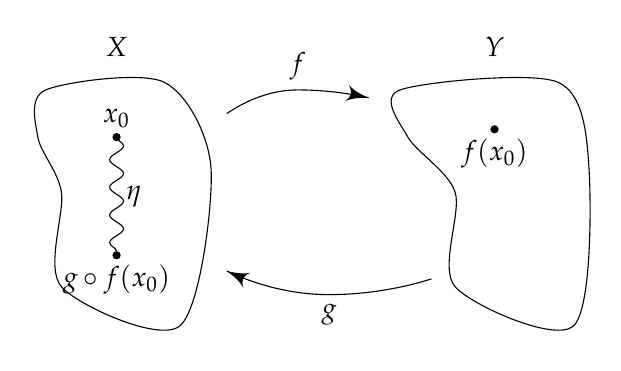
\begin{tikzpicture}
      \draw plot [smooth cycle] coordinates {(-3.7, -1.2) (-3.7, 0) (-4, 0.7) (-3.9, 1.3) (-2.4, 1.4) (-1.8, 0.3) (-2.2, -1.7)};
      \draw plot [smooth cycle] coordinates {(1.3, -1.2) (1.3, 0) (0.7, 0.7) (0.6, 1.3) (2.6, 1.4) (3, 0.3) (2.8, -1.7)};

      \node [circ] at (-3, 0.7) {};
      \node [above] at (-3, 0.7) {$x_0$};
      \node [above] at (-3, 1.6) {$X$};

      \node [above] at (1.8, 1.6) {$Y$};

      \node [circ] at (1.8, 0.8) {};
      \node [below] at (1.8, 0.8) {$f(x_0)$};

      \node [circ] at (-3, -0.8) {};
      \node [below] at (-3, -0.8) {$g\circ f(x_0)$};

      \draw [decoration={snake}, decorate] (-3, 0.7) -- (-3, -0.8) node [right, pos=0.5] {$\eta$};

      \draw [->] (-1.6, 1) parabola bend (-0.7, 1.3) (0.2, 1.2);
      \node [above] at (-0.7, 1.3) {$f$};

      \draw [->] (1, -1.1) parabola bend (-0.3, -1.3) (-1.6, -1);
      \node [below] at (-0.3, -1.3) {$g$};
    \end{tikzpicture}
  \end{center}
  We have no guarantee that $g\circ f(x_0) = x_0$, but we know that our homotopy $H'$ gives us $\eta = H'(x_0, \ph): x_0 \leadsto g\circ f(x_0)$.

  Applying our previous lemma with $\id_X$ for ``$f$'' and $g \circ f$ for ``$g$'', we get
  \[
    \eta_\# \circ (\id_X)_* = (g\circ f)_*
  \]
  Using the properties of the $_*$ operation, we get that
  \[
    g_*\circ f_* = \eta_\#.
  \]
  However, we know that $\eta_\#$ is an isomorphism. So $f_*$ is injective and $g_*$ is surjective.

  Doing it the other way round with $f\circ g$ instead of $g\circ f$, we know that $g_*$ is injective and $f_*$ is surjective. So both of them are isomorphisms.
\end{proof}


\begin{defn}[Simply connected space]
  A space $X$ is \textbf{simply connected} if it is path connected \textbf{and} $\pi_1(X, x_0) \cong 1$ for some (any) choice of $x_0 \in X$.
\end{defn}

\begin{example}
  Clearly, a point $*$ is simply connected since there is only one path on $*$ (the constant path). Hence, any contractible space is simply connected since it is homotopic to $*$. For example, $\R^n$ is simply connected for all spaces.
\end{example}



There is an important theorem, called the van Kampen theorem, for computations of fundamental groups. In the following, you will find the simple version of the theorem.
\begin{thm}[Simple version of van Kampen theorem]
If $X = U_1 \cup U_2$ with $U_i$ open and path-connected, and $U_1 \cap U_2$
path-connected and simply connected, then there is an isomorphism $\ \pi_1(U_1) * \pi_1(U_2) \cong \pi_1(X)$.
\end{thm}
Due to time limit, I have to omit general version of van Kampen theorem. 
If you are interested in it, you can read the book of Hatcher \cite[\S1.2]{Hatcher}.










\subsubsection{Covering space}

Intuitively, a \emph{covering space} of $X$ is a pair $(\tilde{X}, p: \tilde{X} \to X)$, such that if we take any $x_0 \in X$, there is some neighbourhood $U$ of $x$ such that the pre-image of the neighbourhood is ``many copies'' of $U$.
\begin{center}
  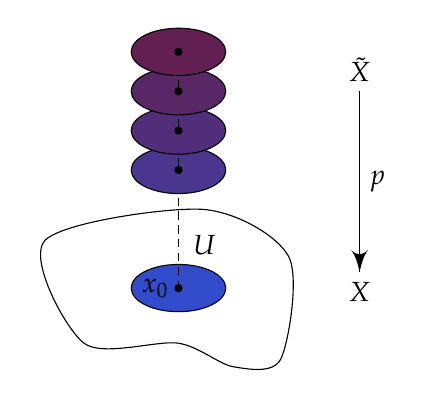
\begin{tikzpicture}
    \draw plot [smooth cycle] coordinates {(-1.2, -0.7) (0, -0.7) (0.7, -1) (1.3, -0.9) (1.4, 0.4) (0.3, 1) (-1.7, 0.6)};

    \draw [fill=mblue] ellipse (0.6 and 0.3);
    \node at (0.6, 0.3) [anchor = south east] {$U$};

    \draw [densely dashed] (0, 1.5) -- (0, 0);
    \foreach \y in {1.5, 2, 2.5, 3} {
      \node [circ] at (0, \y) {};
      \pgfmathsetmacro\c{100 - \y * 20};
      \draw [densely dashed] (0, \y) -- (0, \y - 0.5);
      \draw [fill=mblue!\c!mred] (0, \y) ellipse (0.6 and 0.3);
      \node [circ] at (0, \y) {};
    }
    \node [circ] at (0, 0) {};
    \node [left] at (0, 0) {$x_0$};

    \draw [->] (2.3, 2.5) node [above] {$\tilde{X}$}-- +(0, -2.3) node [pos=0.5, right] {$p$} node [below] {$X$};
  \end{tikzpicture}
\end{center}



\begin{example}
  Consider $p_n: S^1 \to S^1$ (for any $n \in \Z\setminus\{0\}$) defined by $z \mapsto z^n$. We can consider this as ``winding'' the circle $n$ times, or as the following covering map:
  \begin{center}
    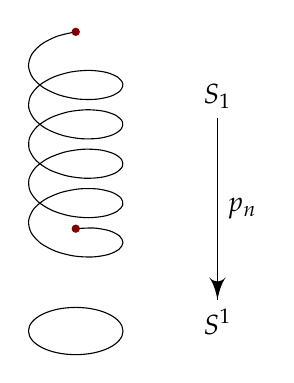
\begin{tikzpicture}
      \draw [samples=80, domain=0:5] plot [smooth] ({0.6 * sin (360 * \x)}, {1 + 0.3 * cos (360 * \x) + \x / 2});
      \node [circ, mred] at (0, 1.3) {};
      \node [circ, mred] at (0, 3.8) {};

      \draw ellipse (0.6 and 0.3);

      \draw [->] (1.8, 2.7) node [above] {$S_1$}-- +(0, -2.3) node [pos=0.5, right] {$p_n$} node [below] {$S^1$};
    \end{tikzpicture}
  \end{center}
  where we join the two red dots together.

  This time the pre-image of $1$ would be $n$ copies of $1$, instead of $\Z$ copies of $1$.
\end{example}

\begin{example}
  Consider $X = \RP^2$, which is the real projective plane. This is defined by $S^2/{\sim}$, where we identify every $x\simeq -x$, i.e.\ every pair of antipodal point. In fact, the quotient map $p: S^2 \to \RP^2$ is indeed a covering map, since the pre-image of a small neighbourhood of any $x_0$ is just two copies of the neighbourhood.  \begin{center}
    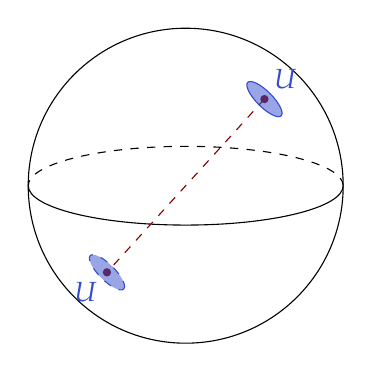
\begin{tikzpicture}
      \draw circle [radius=2];

      \draw [dashed] (2, 0) arc (0:180:2 and 0.5);
      \draw (-2, 0) arc (180:360:2 and 0.5);

      \draw [dashed, mred] (1, 1.1) node [circ] {} -- (-1, -1.1) node [circ] {};

      \draw [rotate around={-45:(1, 1.1)}, mblue, fill=mblue, fill opacity=0.5] (1, 1.1) ellipse (0.3 and 0.1) node [opacity=1, anchor = south west] {$U$};

      \draw [dashed, rotate around={-45:(-1, -1.1)}, mblue, fill=mblue, fill opacity=0.5] (-1, -1.1) ellipse (0.3 and 0.1) node [opacity=1, anchor = north east] {$U$};
    \end{tikzpicture}
  \end{center}

\end{example}



\begin{defn}[Universal cover]
  A covering map $p: \tilde{X} \to X$ is a \textbf{universal cover} if $\tilde{X}$ is simply connected.
\end{defn}







\subsection{Homotopy group}

Let $I^n$ ($n\ge1$) denote the unitn-cube $I\times \cdots \times I$,
The boundary $\partial I^n$ is the geometrical boundary of $I^n$.
As in the fundamental group, we assume here that we shall be concerned with continuous maps $\alpha : I^n \to X$, which map the boundary $\partial I^n$ to a point $x_0 \in X$. Since the boundary is mapped to a single point $x_0$. The map $\alpha$ is called an $n$-loop at $x_0$. 

\begin{defn}[Homotopy class]
 Let $X$ be a topological space. The set of homotopy classes of $n$-loops ($n \ge 1$) at $x_0 \in X$ is denoted by $\pi_n(X, x_0)$ and called the $n$-th homotopy group at $x_0$. $\pi_n(X, x_0)$ is called the higher homotopy group if $n \ge 2$.
 \end{defn}
 
The product $\alpha * \beta$  just defined naturally induces a product of homotopy classes defined by
 $$[\alpha] * [\beta]=[\alpha * \beta] $$
\begin{figure}[h]\centering
\includegraphics[width=8cm]{homotopy-group}
\end{figure}



 Higher homotopy groups are always Abelian; for any $n$-loops $\alpha$ and $\beta$ at $x_0 \in X$, $[\alpha]$ and $[\beta]$  satisfy
$$[\alpha] * [\beta] = [\beta] * [\alpha].$$
 
 
\begin{figure}[h]\centering
\includegraphics[width=\textwidth]{homotopy-group2}
\end{figure}

\subsubsection{Global $SU(2)$ anomaly}
There are various applications of homotopy groups to physics. Here I just give you one example.

Let us consider the path integral of a gauge theory with chiral fermion $\psi$ in a representation $R$ of $G$.
\begin{equation}
Z[A_\mu] = \int [{\cal D} \psi][{\cal D}\bar\psi] e^{-\int \bar\psi D_\mu \sigma^\mu \psi}
\end{equation}  
To perform a further integration over $A_\mu$ consistently, we need \begin{equation}
Z[A_\mu]= Z[A^g_\mu], \quad A^g_\mu = g^{-1} A_\mu g  + g^{-1} \partial_\mu g.
\end{equation} for any gauge transformation $g:\mathbb{R}^4\to G$. We will learn it in a subsequent lecture about gauge transformation of non-Abelian gauge theory.


When we consider odd number of chiral fermions in the doublet of $\SU(2)$ gauge group, Witten has shown that there is a global anomaly \cite{Witten:1982fp}.
Since continuous change of $g$ does not change the phase of $[{\cal D}\psi][{\cal D}\bar \psi]$, we need to consider maps $g:\mathbb{R}^4\to \SU(2)$ up to continuous change. Upon one-point compactifiction of $\bR^4$ to $S^4$,
they are characterized by $\pi_4(\SU(2))$, which is known  
\begin{equation}
\pi_4(\SU(2))=\pi_4(S^3)=\mathbb{Z}_2~.
\end{equation} Let $g_0:\mathbb{R}^4\to \SU(2)$ be the gauge transformation corresponding to the nontrivial element in this $\bZ_2$.  
It is known that  $[{\cal D}\psi][{\cal D}\bar \psi]$ gets a minus sign  under this gauge transformation.
So, one cannot have an odd number of Weyl fermions in the doublet representation of gauge group $\SU(2)$. 






\section{Lecture 7: \cite{Nakahara} \S 3}



\subsection{Simplicial complexes}

The relevance is that these can be used to define simplexes (which are simple, as opposed to complexes).
\begin{defn}[$n$-simplex]
  An \textbf{$n$-simplex} is the convex hull of $(n + 1)$ affinely independent points $a_0, \cdots, a_n \in \bR^m$, i.e.\ the set
  \[
    \sigma = \langle a_0, \cdots, a_n\rangle = \left\{\sum_{i = 0} t_i a_i : \sum_{i = 0}^n t_i = 1,t_i \geq 0\right\}.
  \]
  The points $a_0, \cdots, a_n$ are the \textbf{vertices}, and are said to \textbf{span} $\sigma$. The $(n + 1)$ tuples $(t_0, \cdots, t_n)$ are called the \textbf{barycentric coordinates} for the point $\sum t_i a_i$.
  
  

  We often denote an oriented simplex as $\sigma$, and then $\bar{\sigma}$ denotes the same simplex with the opposite orientation.
\end{defn}

Some examples are as follows. When $n=0$, it is a point. $n=1$, it is a line.

  \begin{minipage}[b]{2.5cm}  
 \begin{center}
    \begin{tikzpicture}
      \node [circ] at (0,1) {};
        \node at (0,0) {$n=0$};
    \end{tikzpicture}  
  \end{center}
      \end{minipage}
  \begin{minipage}[b]{3.5cm} 
   \begin{center}
    \begin{tikzpicture}
      \node [circ] at (0, 0) {};
      \node [circ] at (2, 0) {};
      \draw (0, 0) -- (2, 0);
              \node at (1,-1) {$n=1$};
    \end{tikzpicture}
  \end{center}
      \end{minipage}
  \begin{minipage}[b]{3.5cm}
  \begin{center}
    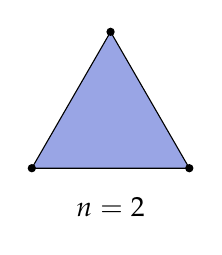
\begin{tikzpicture}
      \draw [fill=mblue, fill opacity=0.5] (0, 0) -- (2, 0) -- (1, 1.732) -- cycle;
      \node [circ] at (0, 0) {};
      \node [circ] at (2, 0) {};
      \node [circ] at (1, 1.732) {};
                    \node at (1,-.5) {$n=2$};
    \end{tikzpicture}
  \end{center}
    \end{minipage}
  \begin{minipage}[b]{3.5cm}
  \begin{center}
    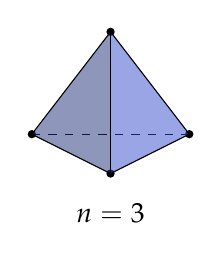
\begin{tikzpicture}
      \node [circ] at (0, 0) {};
      \node [circ] at (2, 0) {};
      \node [circ] at (1, -0.5) {};
      \node [circ] at (1, 1.3) {};
      \draw [dashed] (0, 0) -- (2, 0);
      \fill [mblue, opacity=0.5] (2, 0) -- (1, -0.5) -- (1, 1.3) -- cycle;
      \fill [mblue!60!black, opacity=0.5] (0, 0) -- (1, -0.5) -- (1, 1.3) -- cycle;
      \draw (2, 0) -- (1, -0.5) -- (0, 0);
      \draw (0, 0) -- (1, 1.3) -- (2, 0);
      \draw (1, 1.3) -- (1, -0.5);
                          \node at (1,-1) {$n=3$};
    \end{tikzpicture}
  \end{center}
  \end{minipage}

  A \textbf{face} of a simplex is a subset (or subsimplex) spanned by a subset of the vertices. The \textbf{boundary} is the union of the proper faces, and the \textbf{interior} is the complement of the boundary. The boundary of $\sigma$ is usually denoted by $\partial \sigma$, while the interior is denoted by $\mathring{\sigma}$, and we write $\tau \leq \sigma$ when $\tau$ is a face of $\sigma$. In particular, the interior of a vertex is the vertex itself. Note that this notion of interior and boundary is distinct from the topological notion of boundary.
  
  
  
  

\begin{example}
  The \textbf{standard $n$-simplex} is spanned by the basis vectors $\{\mathbf{e}_1, \cdots, \mathbf{e}_n\}$ in $\bR^{n + 1}$. For example, when $n = 2$, we get the following:
  \begin{center}
    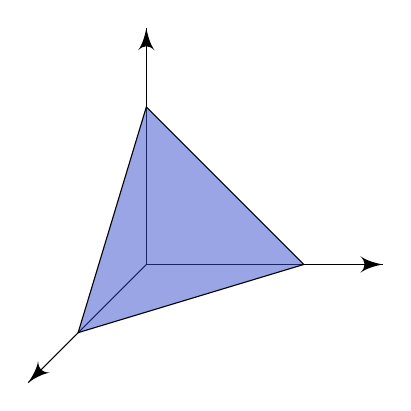
\begin{tikzpicture}
      \draw [->] (0, 0) -- (3, 0);
      \draw [->] (0, 0) -- (0, 3);
      \draw [->] (0, 0) -- (-1.5, -1.5);

      \draw [fill=mblue, fill opacity=0.5] (0, 2) -- (2, 0) -- (-.866, -0.866) -- cycle;
    \end{tikzpicture}
  \end{center}
\end{example}

We will now glue simplices together to build \textbf{complexes}, or \textbf{simplicial complexes}.

\begin{defn}
  A \textbf{simplicial complex} is a finite set $K$ of simplices in $\bR^n$ such that
  \begin{enumerate}
    \item If $\sigma \in K$ and $\tau$ is a face of $\sigma$, then $\tau \in K$.
    \item If $\sigma, \tau \in K$, then $\sigma \cap \tau$ is either empty or a face of both $\sigma$ and $\tau$.
  \end{enumerate}
\end{defn}



\begin{example}
  This is a simplicial complex:
  \begin{center}
    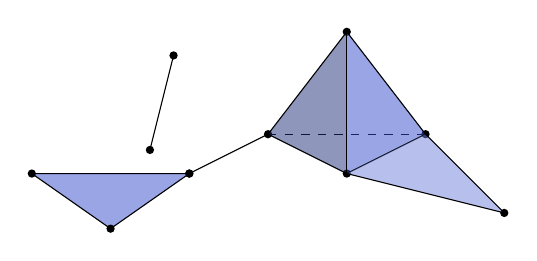
\begin{tikzpicture}
      \node [circ] at (0, 0) {};
      \node [circ] at (2, 0) {};
      \node [circ] at (3, -1) {};
      \node [circ] at (1, -0.5) {};
      \node [circ] at (1, 1.3) {};
      \node [circ] at (-1, -0.5) {};
      \draw [dashed] (0, 0) -- (2, 0);
      \fill [mblue, opacity=0.5] (2, 0) -- (1, -0.5) -- (1, 1.3) -- cycle;
      \fill [mblue!60!black, opacity=0.5] (0, 0) -- (1, -0.5) -- (1, 1.3) -- cycle;
      \draw (2, 0) -- (1, -0.5) -- (0, 0);
      \draw (0, 0) -- (1, 1.3) -- (2, 0);
      \draw (1, 1.3) -- (1, -0.5);
      \draw [fill=mblue!70!white, fill opacity=0.5] (2, 0) -- (3, -1) -- (1, -0.5);

      \draw (0, 0) -- (-1, -0.5);
      \draw [fill=mblue, fill opacity=0.5] (-3, -0.5) -- (-1, -0.5) -- (-2, -1.2) -- cycle;
      \node [circ] at (-3, -0.5) {};
      \node [circ] at (-1, -0.5) {};
      \node [circ] at (-2, -1.2) {};

      \draw (-1.5, -0.2) node [circ] {} -- (-1.2, 1) node [circ] {};
    \end{tikzpicture}
  \end{center}
\end{example}
Technically, a simplicial complex is defined to be a set of simplices, which is just collections of points. It is not a subspace of $\bR^n$.  The \textbf{polyhedron} defined by $K$ is the union of the simplices in $K$, and denoted by $|K|$.  The \textbf{dimension} of $K$ is the highest dimension of a simplex of $K$. The \textbf{$d$-skeleton} $K^{(d)}$ of $K$ is the union of the $n$-simplices in $K$ for $n \leq d$.
  A \textbf{triangulation} of a space $X$ is a homeomorphism $h: |K| \to X$, where $K$ is some simplicial complex.


\begin{example}
  Let $\sigma$ be the standard $n$-simplex. The boundary $\partial \sigma$ is homeomorphic to $S^{n - 1}$ (e.g.\ the boundary of a (solid) triangle is the boundary of the triangle, which is also a circle) . This is called the \textbf{simplicial $(n - 1)$ sphere}.
\end{example}

We can also triangulate our $S^n$ in a different way:
\begin{example}
  In $\bR^{n + 1}$, consider the simplices $ \langle \pm \mathbf{e}_0, \cdots, \pm \mathbf{e}_n\rangle$ for each possible combination of signs. So we have $2^{n + 1}$ simplices in total. Then their union defines a simplicial complex $K$, and
  \[
    |K| \cong S^n.
  \]
  \begin{center}
    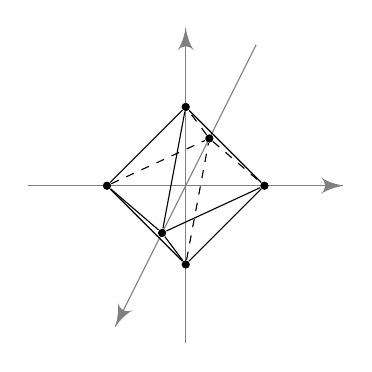
\begin{tikzpicture}
      \draw [gray, ->] (-2, 0) -- (2, 0);
      \draw [gray, ->] (0, -2) -- (0, 2);
      \draw [gray, ->] (0.894, 1.788) -- (-0.894, -1.788);

      \node [circ] (x1) at (1, 0) {};
      \node [circ] (x2) at (-1, 0) {};
      \node [circ] (z1) at (0, 1) {};
      \node [circ] (z2) at (0, -1) {};
      \node [circ] (y1) at (-0.3, -0.6) {};
      \node [circ] (y2) at (0.3, 0.6) {};

      \draw (x1) -- (y1) -- (z1) -- (x1) -- (z2) -- (y1) -- (x2) -- (z1);
      \draw (z2) -- (x2);
      \draw [dashed] (x2) -- (y2) -- (x1);
      \draw [dashed] (z2) -- (y2) -- (z1);
    \end{tikzpicture}
  \end{center}
\end{example}
The nice thing about this triangulation is that the simplicial complex is invariant under the antipodal map. So not only can we think of this as a triangulation of the sphere, but a triangulation of $\RP^n$ as well.





    An \textbf{oriented $n$-simplex} in a simplicial complex $K$ is an $n + 1$-tuple $(a_0, \cdots, a_n)$ of vertices $a_i \in V_k$ such that $\langle a_0, \cdots, a_n\rangle \in K$, where we think of two $n + 1$ tuples $(a_0, \cdots, a_n)$ and $(a_{\pi(0)}, \cdots, a_{\pi(n)})$ as the same \textbf{oriented} simplex if $\pi \in S^n$ is an \textbf{even} permutation.
    
    
    
\begin{defn}[Chain group $C_n(K)$]
  Let $K$ be a simplicial complex. 
  Let $\{\sigma_1, \cdots, \sigma_\ell\}$ be the set of $n$-simplices of $K$ with orientation. Then we define $C_n(K)$ be the free abelian group with basis $\{\sigma_1, \cdots, \sigma_\ell\}$, i.e.\ $C_n(K) \cong \Z^\ell$.
\end{defn}


  We define \textbf{boundary homomorphisms}
  \[
    \partial_n: C_n(K) \to C_{n - 1}(K)
  \]
  by
  \[
    (a_0, \cdots, a_n) \mapsto \sum_{i = 0}^n (-1)^i (a_0, \cdots, \hat{a}_i, \cdots, a_n),
  \]
  where $(a_0, \cdots, \hat{a}_i, \cdots, a_n) = (a_0, \cdots, a_{i - 1}, a_{i + 1}, a_n)$ is the simplex with $a_i$ removed. We can show that $\partial_{n+1}\cdot \partial_n=0$.




We will develop some formalism to help us compute homology groups $H_k(K)$ in lots of examples. 
\begin{defn}[Chain complex and differentials]
  A \textbf{chain complex} $C_{\bullet}$ is a sequence of chain groups $C_0, C_1, C_2, \cdots$ equipped with boundary maps $\partial_n: C_n \to C_{n - 1}$ such that $\partial_{n - 1} \circ \partial_n = 0$ for all $n$.
\end{defn}
\[
  \begin{tikzcd}
  \cdots \ar [r, "\partial_3"'] & C_2 \ar [r, "\partial_2"']   &   C_1 \ar [r, "\partial_1"'] &C_0 \ar[r, "\partial_0"'] &    0 
  \end{tikzcd}
\]

As in the de Rham cohomology, we define the \textbf{$n$-cycles} is 
  \[
    Z_n(C) = \Ker \partial_n.
  \]
  The \textbf{$n$-boundaries} is
  \[
    B_n(C) = \Im \partial_{n+1}.
  \]
Then,  the \textbf{$n$-th homology group} of $C_{\bullet}$ is defined to be
  \[
    H_n(C) = \frac{\Ker \partial_n}{\Im \partial_{n + 1}} = \frac{Z_n(C)}{B_n(C)}.
  \]
  
  
Let  $K\to X$ be a triangulation of an $n$-dimensional compact oriented closed connected manifold $X$. Then, the $n$-th homology is $H_n(K,\Z)\cong \Z$ and its generator is denoted by $[X]$ and called the \textbf{fundamental  class}. 
  

  The \textbf{Euler characteristic} of a triangulated space $h: |K| \to X$ is the alternative sum of real-valued homology groups of $|K|$
  \[
    \chi(X) = \sum_{i \geq 0} (-1)^i \dim_\R H_i(K; \R).
  \]
As we will see below, this  depends only on the homotopy type of $X$. 

\begin{example}
  Let $K$ be the standard simplicial $1$-sphere, ie, we have the following in $\R^3$.
  \begin{center}
    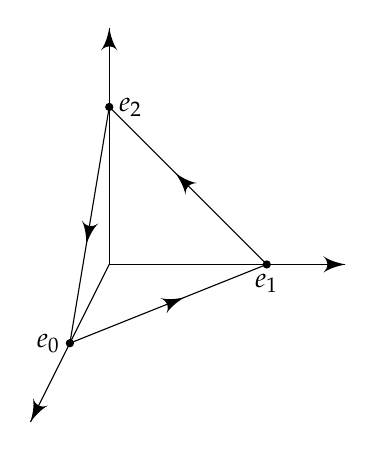
\begin{tikzpicture}
      \draw [->] (0, 0) -- (3, 0);
      \draw [->] (0, 0) -- (0, 3);
      \draw [->] (0, 0) -- (-1, -2);

      \draw [->-=0.58] (2, 0) -- (0, 2);
      \draw [->-=0.58] (0, 2) -- (-0.5, -1);
      \draw [->-=0.58] (-0.5, -1) -- (2, 0);

      \node [left] at (-0.5, -1) {$e_0$};
      \node [below] at (2, 0) {$e_1$};
      \node [right] at (0, 2) {$e_2$};

      \node [circ] at (-0.5, -1) {};
      \node [circ] at (2, 0) {};
      \node [circ] at (0, 2) {};
    \end{tikzpicture}
  \end{center}
  Our simplices are thus
  \[
    K = \{\langle e_0\rangle, \langle e_1\rangle, \langle e_2\rangle, \langle e_0, e_1\rangle, \langle e_1, e_2\rangle, \langle e_2, e_0\rangle\}.
  \]
  Our chain groups are
  \begin{align*}
    C_0(K) &= \langle (e_0), (e_1), (e_2)\rangle \cong \Z^3\\
    C_1(K) &= \langle (e_0, e_1), (e_1, e_2), (e_2, e_0)\rangle \cong \Z^3.
  \end{align*}
  All other chain groups are zero. Note that our notation is slightly confusing here, since the brackets $\langle \ph \rangle$ can mean the simplex spanned by the vertices, or the group generated by certain elements. However, you are probably clueful enough to distinguish the two use cases.

  Hence, the only non-zero boundary map is
  \[
    \partial_1: C_1(K) \to C_0(K).
  \]
  We can write down its matrix with respect to the given basis.
  \[
    \begin{pmatrix}
      -1 & 0 & 1\\
      1 & -1 & 0\\
      0 & 1 & -1
    \end{pmatrix}
  \]
  We have now everything we need to know about the homology groups, and we just need to do some linear algebra to figure out the image and kernel, and thus the homology groups. We have
  \[
    H_0(K) = \frac{\Ker (\partial_0: C_0(K) \to C_{-1}(K))}{\Im (\partial_1: C_1(K) \to C_0(K))} \cong \frac{C_0(K)}{\Im \partial_1} \cong \frac{\Z^3}{\Im \partial_1}.
  \]
  After doing some row operations with our matrix, we see that the image of $\partial_1$ is a two-dimensional subspace generated by the image of two of the edges. Hence we have
  \[
    H_0(K) = \Z.
  \]
  What does this $H_0(\Z)$ represent? We initially said that $H_k(K)$ should represent the $k$-dimensional holes, but when $k = 0$, this is simpler. As for $\pi_0$, $H_0$ just represents the path components of $K$. We interpret this to mean $K$ has one path component. In general, if $K$ has $r$ path components, then we expect $H_0(K)$ to be $\Z^r$.

  Similarly, we have
  \[
    H_1(K) = \frac{\Ker \partial_1}{\Im \partial_2} \cong \Ker \partial_1.
  \]
  It is easy to see that in fact we have
  \[
    \Ker \partial_1 = \langle (e_0, e_1) + (e_1, e_2) + (e_2, e_0)\rangle \cong \Z.
  \]
  So we also have
  \[
    H_1(K) \cong \Z.
  \]
  We see that this $H_1(K)$ is generated by precisely the single loop in the triangle. The fact that $H_1(K)$ is non-trivial means that we do indeed have a hole in the middle of the circle.
\end{example}

We can also consider a map between two simplicial complexes.

\begin{defn}[Simplicial map]
  A \textbf{simplicial map} $f: K \to L$ is a function $f: V_K \to V_L$ such that if $\langle a_0, \cdots, a_n\rangle$ is a simplex in $K$, then $\{f(a_0), \cdots, f(a_n)\}$ spans a simplex of $L$.
\end{defn}


Given triangulations $|K|\to X$ and $|L|\to Y$ for manifolds $X$ and $Y$ and a continuous map $f:X\to Y$, we can ``approximate'' $f$ by a simplicial map $g:K\to L$. (See \cite[p.177]{Hatcher} for more detail.)

In fact, a simplicial map $f$ induces a map between simplicial complexes.



\begin{defn}[Chain map]
  A chain map $f_{\bullet}: C_{\bullet}\to D_{\bullet}$ is a sequence of homomorphisms $f_n: C_n \to D_n$ such that
  \[
    f_{n - 1} \circ \partial_n = \partial_n \circ f_n
  \]
  for all $n$. In other words, the following diagram commutes:
  \[
    \begin{tikzcd}[row sep=large]
 \cdots \ar [r, "\partial_3"']&  C_2 \ar [r, "\partial_2"'] \ar [d, "f_2"'] &   C_1 \ar [r, "\partial_1"'] \ar[d, "f_1"'] & C_0 \ar[r, "\partial_0"'] \ar[d, "f_0"'] &   0   \\
\cdots \ar [r, "\partial_3"]&  D_2 \ar [r, "\partial_2"] &   D_1 \ar [r, "\partial_1"] & D_0 \ar[r, "\partial_0"] &   0
    \end{tikzcd}
  \]
\end{defn}



%Here, $K$ is always a simplicial complex, and $C_{\bullet} = C_{\bullet}(K)$.

  Let $f: K \to L$ be a simplicial map. Then $f$ induces a chain map $f_{\bullet}: C_{\bullet}(K) \to C_{\bullet}(L)$. Hence it also induces $f_*: H_n (K) \to H_n(L);[c] \mapsto [f(c)]$. In fact, given triangulations $|K|\to X$ and $|L|\to Y$ for homotopically equivalent manifolds $f:X \to Y$ with $f\sim \id$, its simplicial approximation $g:K\to L$ induces an isomorphism $g_*: H_n (K) \cong H_n(L)$.





\subsection{Mayer-Vietoris sequence}


Here I just give you introduction to a powerful theorem called Mayer-Vietoris sequence to compute homology. For more detail, I refer to \cite[p.149]{Hatcher}.

Suppose we have a space $K = M\cup N$, where $M \cap N$ are path-connected.
\begin{center}
  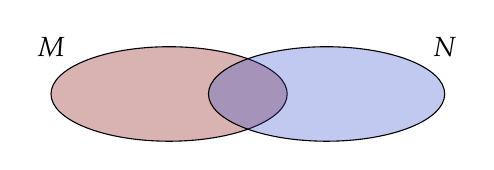
\begin{tikzpicture}
    \draw [fill=mred, fill opacity=0.3] (-1, 0) ellipse (1.5 and 0.6);
    \draw [fill=mblue, fill opacity=0.3] (1, 0) ellipse (1.5 and 0.6);
    \node at (-2.5, 0.6) {$M$};
    \node at (2.5, 0.6) {$N$};
  \end{tikzpicture}
\end{center}
The theorem tells us how to compute the homology of the union $M\cup N$ in terms of those of $M, N$ and $M\cap N$.


\begin{thm}[Mayer-Vietoris theorem]
  Let $K, L, M, N$ be simplicial complexes with $K = M\cup N$ and $L = M\cap N$. We have the following inclusions and maps:
  \[
    \begin{tikzcd}
      L \ar[r, hook, "i"] \ar[d, hook, "j"] & M\ar[d, hook, "k"]\\
      N \ar[r, hook, "\ell"] & K.
    \end{tikzcd}
  \]
  Then there exists some natural homomorphism $p_*: H_n(K) \to H_{n - 1}(L)$ that gives the following long exact sequence:
  \[
    \begin{tikzcd}
      \cdots \ar[r, "p_*"] & H_n(L) \ar[r, "i_* + j_*"] & H_n(M) \oplus H_n(N) \ar[r, "k_* - \ell_*"] & H_n(K)\ar[out=0, in=180, looseness=2, overlay, lld, "p_*"']\\
      & H_{n - 1}(L) \ar[r, "i_* + j_*"] & H_{n - 1}(M) \oplus H_{n - 1}(N) \ar[r, "k_* - \ell_*"] & H_{n - 1}(K) \ar [r] & \cdots\\
      &\cdots \ar[r] & H_0(M) \oplus H_0(N) \ar[r, "k_* - \ell_*"] & H_0(K) \ar [r] & 0
    \end{tikzcd}
  \]
\end{thm}
Here $A \oplus B$ is the direct sum of the two (abelian) groups, which may also be known as the Cartesian product.



\subsection{de Rham theorem and Poincare duality}
Given a simplicail complex $K$ and its chain group $C_k(K)$, we can define \textbf{cochain group}
$$
C^k(K)=\{ f:C_k(K)\to \Z \  \textrm{homomorphism}\}
$$ 
In addition, we can define \textbf{coboundary} $\delta:C^k(K)\to C^{k+1}(K)$ as $\delta f(c)=f(\partial c)$ were $c\in C_{k+1}(K)$. It is easy to see $\delta\cdot \delta =0$. We can define \textbf{cocycle} $Z^k(K)=\Ker\delta$ and \textbf{coboundary} $B^k(K)=\Im\delta$. The cohomology group of $K$ is defined by 
$$
H^k(K)=Z^k(K)/B^k(K)~.
$$
There exists bilinear map
$$
H_k(K)\otimes H^k(K)\to \Z; ([c],[f])\mapsto f(c)
$$
which is well defined.






\begin{thm}[de Rham]
Let $X$ be a smooth manifold and $|K|\to X$ be its triangulation. Then, we have an isomorphism
$$
H^*_{dR}(X)\cong H^*(K,\bR)~.
$$
\end{thm}



In fact, there is a relation between homology group and cohomology group. A $k$-dimensional oriented submanifold $Y\subset X$ without boundary indeed represents a generator $[Y]\in H_k(X)$. The definition of a submanifold is given in section 5.2.7 of Nakahara. There exists $\eta\in H^{n-k}(X)$ such that
$$
\int_Y \omega =\int_X\omega\wedge \eta
$$
for any $\omega\in H^k(X)$.

\begin{thm}[Poincare duality]
Let $X$ be an $n$-dimensional compact oriented closed manifold. Then, we have an isomorphism
$$
\vartheta: H_{k}(X)\cong H^{n-k}(K,\bR); Y\mapsto \eta
$$
\end{thm}

Using this isomorphism, one can define an \textbf{intersection number} $Y_1\cdot Y_2$ for $Y_1\in H^k(X)$ and $Y_2\in H^{n-k}(X)$.
$$
Y_1\cdot Y_2:=\int_X \eta_1\wedge \eta_2
$$
where $\vartheta(Y_i) =\eta_i$.


\subsection{Lefschetz fixed point theorem and Poincare-Hopf theorem}
Let $X$ and $Y$ be $n$-dimensional smooth closed oriented manifolds. 
A smooth map $f:X\to Y$ induces an homomorphism $f_*:H_*(X)\to H_*(Y)$. In particular, we define \textbf{mapping degree} of $f$ by 
$$
 f_*([X]):=(\deg f) [Y]~.
$$
In the language of cohomology group, we can define
$$
\deg f:= \frac{\int_{X}f^* \omega} {\int_Y\omega}
$$
where $\omega$ is the volume form of $Y$.

Given two knots $K_1,K_2:S^1\to \bR^3$, we can define $F:K_1\times K_2\to S^2$ by
$$
F(p,q)=\frac{x_1-x_2}{|x_1-x_2|}
$$
Then, we define the \textbf{linking number} of $K_1$ and $K_2$ as
$$
Lk(K_1,K_2):=\deg F=\frac{1}{4\pi}\int_{K_1\times K_2} F^* \omega=\frac{1}{4\pi}\int_{K_1}dx_1^i \int_{K_2} dx_2^j \frac{(x_1-x_2)^k}{|x_1-x_2|^3}\epsilon_{ijk}
$$
where $\omega$ is the volume form of $S^2$.
\begin{figure}[h]\centering
\includegraphics{linking}
\end{figure}

This number was first introduced by Gauss in the study of electromagnetism.  Biot-Savart law tells us that the magnetic field generated by electric current running on $K_1$ with unit strength is
$$
\vec{B}(\vec x)= \frac1{4\pi}\int_{K_1}  \frac{(\vec{x}-\vec {x_1}(t_1))^k\times \frac{d\vec {x_1}}{dt_1} }{|\vec x- \vec x_1|^3}dt_1
$$
Therefore, $Lk(K_1,K_2)$ is the energy which costs to move a magnetic monopole along $K_2$ under this magnetic field. Gauss has noticed that the integral always provides an integer however $K_1$ and $K_2$ are drawn. Moreover, this number stays invariant even though you deform $K_1$ and $K_2$!


Let $X$ be an $n$-dimensional smooth closed oriented manifold. 
We assume that a map $f: X \to X$ has isolated fixed points $f(p)=p$. We define a map $h:S^{n-1}_\epsilon\to S^{n-1}$ by
$$
h(q)=\frac{q-f(q)}{|q-f(q)|}
$$
The index of $f$ at the fixed point $p$ is defined by
$$
\textrm{ind}_p f:=\deg h
$$
We define the \textbf{Lefschetz number} of $f$ as
  \[
    L(f) = \sum_{i \geq 0} (-1)^i \tr(f_*: H_i(X; \R) \to H_i(X; \R)).
  \]

\begin{thm}[Lefschetz fixed point theorem]
Lefschetz number is the sum of indices over isolated fixed points
$$
 L(f)=\sum_{p} \textrm{ind}_p f
$$
\end{thm}
\begin{minipage}[b]{6.5cm}
\includegraphics[width=5.5cm]{vector-fields}
\end{minipage}
\begin{minipage}[b]{8cm}
\includegraphics[width=8.5cm]{vector-field-indices}
\end{minipage}

Let $v$ is a vector field on $X$ and $\varphi_t$ is a flow generated by $v$. Then, the index of a zero point $p$ of $v$ is defined by
$$
\textrm{ind}_p v =\textrm{ind}_p \varphi_t~.
$$
Since the flow $\varphi_t$ is homotopic to the identity $\varphi_t\sim id$, $L(\varphi_t)$ is equal to the Euler characteristic.
$$
    L(\varphi_t) =\sum_{i \geq 0} (-1)^i \tr(id: H_i(X; \R) \to H_i(X; \R)).=\sum_{i \geq 0} (-1)^i \dim H_i(X; \R) =\chi(X)
$$
Therefore, we obtain:
\begin{thm}[Poincare-Hopf theorem]
The Euler characteristics is the sum of indices over isolated fixed points
$$
\chi(X)=\sum_{p} \textrm{ind}_p v
$$
\end{thm}
This theorem was introduced in the first lecture.



\section{Lecture 8: \cite{Nakahara} \S 5.6, 5.7, 9.3}



\subsection{Lie groups and Lie algebras}


\begin{defn}[Lie group]\index{Lie group}
  A \textbf{Lie group} is a manifold $G$ with a group structure such that multiplication $m: G \times G \to G$ and inverse $i: G \to G$ are smooth maps. The \textbf{dimension} of a Lie group $G$ is the dimension of the underlying manifold.
\end{defn}

  For each $h \in G$, we define the \textbf{left and right translation maps}
  \begin{align*}
    L_h: G &\to G;  g \mapsto hg~,\\
    R_h: G &\to G; g \mapsto gh~.
  \end{align*}
  These maps are bijections, and in fact diffeomorphisms (i.e.\ smooth maps with smooth inverses), because they have smooth inverse $L_{h^{-1}}$ and $R_{h^{-1}}$ respectively.



In general, Lie group will be given by subsets of Euclidean space specified by certain algebraic equations, but note that not all subsets given by equations are manifolds, and it is possible that they have some singularities.

\begin{example}
Here are some examples.


\begin{itemize}
\item  general linear group: $\GL(n, \bF) = \{A \in \textrm{M}_n(\bF)| \det A \neq 0\}$
\item  special linear group: $\SL(n, \bF) = \{A \in \GL(n, \bF)| \det A = 1\}$
\item Unitary group $\U(n) = \{A \in \GL(n, \bC)| AA^\dagger = I\}$
\item Special unitary group $\SU(n) =\{A \in \U(n)| \det A = 1\}$
\item  Orthogonal group $\mathrm{O}(n) =  \{A \in \GL(n, \bR)| AA^T = I\}$
\item Special orthogonal group $\SO(n) = \{A \in \mathrm{O}(n)| \det A = 1\}$
\end{itemize}
\end{example}



\begin{defn}[Lie algebra]\index{Lie algebra}
  A \textbf{Lie algebra} $\mathfrak{g}$ is a vector space (over $\bF=\bR$ or $\bC$) with a \term{bracket}
  \[
    [\ph,\ph] : \mathfrak{g} \times \mathfrak{g} \to \mathfrak{g}
  \]
  satisfying
  \begin{enumerate}
      \item $[\alpha X + \beta Y, Z] = \alpha [X, Z] + \beta [Y, Z]$ for all $X, Y, Z \in \mathfrak{g}$ and $\alpha, \beta \in \bF$ \hfill(bilinearity)
    \item $[X, Y] = -[Y, X]$ for all $X, Y \in \mathfrak{g}$ \hfill(antisymmetry)
    \item $[X, [Y, Z]] + [Y, [Z, X]] + [Z, [X, Y]] = 0$ for all $X, Y, Z \in \mathfrak{g}$.\hfill(Jacobi identity\index{Jacobi identity})
  \end{enumerate}
  Note that linearity in the second argument follows from linearity in the first argument and antisymmetry.
\end{defn}



We now try to get a Lie algebra from a Lie group $G$, by considering ${T}_e(G)$.
  The tangent space of a Lie group $G$ at the identity naturally admits a Lie bracket
  \[
    [\ph, \ph]: T_e G \times T_e G \to T_e G; (X,Y) \mapsto [X,Y]=XY-YX
  \]
  such that
  \[
    \mathfrak{g} = (T_e(G), [\ph, \ph])
  \]
  is a Lie algebra.
 
\begin{defn}[Lie algebra of a Lie group]\index{Lie algebra of a Lie group}
  Let $G$ be a Lie group. The \textbf{Lie algebra} of $G$, written $\mathfrak{g}$, is the tangent space $T_e G$ under the natural Lie bracket.
\end{defn}
The general convention is that if the name of a Lie group is denoted by capital letters, then the corresponding Lie algebra is the same name with fraktur font. For example, the Lie group of $\SO(n)$ is $\so(n)$.



Given a finite-dimensional Lie algebra, we can pick a basis $B$ for $\mathfrak{g}$.
\be\label{Lie-basis}
  B = \{T_a: a = 1, \cdots, \dim \mathfrak{g}\}.
\ee
Then any $X \in \mathfrak{g}$ can be written as
\[
  X = X^a T_a = \sum_{a = 1}^n X^a T_a,
\]
where $X^a \in \bF$.

By linearity, the bracket of elements $X, Y \in \mathfrak{g}$ can be computed via
\[
  [X, Y] = X^a Y^b [T_a, T_b].
\]
In other words, the whole structure of the Lie algebra can be given by the bracket of basis vectors. We know that $[T_a, T_b]$ is again an element of $\mathfrak{g}$. So we can write
\[
  [T_a, T_b] = f_{ab}{}^c T_c,
\]
where $f_{ab}{}^c\in \bF$ are called the \textbf{structure constants}.
By the antisymmetry of the bracket, we know
  \[
    f_{ba}{}^c = -f_{ab}{}^c.
  \]
The Jacobi identity amounts to
  \[
    f_{ab}{}^c f_{cd}{}^e + f_{da}{}^c f_{cb}{}^e + f_{bd}{}^c f_{ca}{}^e = 0.
  \]




\begin{example}
  Take $G = \SO(3)$. Then $\so(3)$ is the space of $3 \times 3$ real anti-symmetric matrices, which one can manually check are generated by
  \[
    {T}_1 =
    \begin{pmatrix}
      0 & 0 & 0\\
      0 & 0 & -1\\
      0 & 1 & 0
    \end{pmatrix},\quad
    {T}_2 =
    \begin{pmatrix}
      0 & 0 & 1\\
      0 & 0 & 0\\
      -1 & 0 & 0
    \end{pmatrix},\quad
    {T}_3 =
    \begin{pmatrix}
      0 & -1 & 0\\
      1 & 0 & 0\\
      0 & 0 & 0
    \end{pmatrix}
  \]
  We then have
  \[
    ({T}_a)_{bc} = -\varepsilon_{abc}.
  \]
  Then the structure constants are  $f_{ab}{}^{c} = \varepsilon_{abc}$.
\end{example}



Given a vector $X\in \mathfrak{g} $ in the tangent space of the identity $e$, one can generate the vector field by pushing-forward by the left translation $L_g$. Let us denote the corresponding vector field by $X$ too. Since $(L_g)_*X=X$, it is called a \term{left-invariant vector field}.  The flow generated by the vector field $X$ is called \textbf{exponential map}, which can be expressed as a matrix
  \[
    \exp(tX) = \sum_{\ell = 0}^\infty \frac{1}{\ell!} (tX)^\ell~.
  \]
Therefore, for any matrix Lie group $G$, the exponential map defines a map $\exp:\mathfrak{g}  \to G$.

Given a Lie algebra $\frakg$, it is also natural to think about its dual space $\frakg^*$. This can be identified with the set of all left invariant 1-forms $\omega$ on $G$ such that $L_g^*\omega =\omega$. Note that $\omega(X)$, $\omega(Y)$ are constant over $G$ for $\omega\in \frakg^*$ and $X,Y\in \frakg$. Therefore, we have $Y(\omega(X))=0=X(\omega(Y))$ so that
$$
d\omega(X,Y)=\frac12\omega([X,Y])~.
$$
Therefore, if we take the basis $\omega_1,\cdots,\omega_{\dim \frakg}$ dual to \eqref{Lie-basis}, we can write it as
$$
d\omega_i=-\frac12 \sum_{j,k} f_{jk}{}_{i}~\omega_j\wedge \omega_k~.
$$
Moreover, let $\omega\in \Omega^1(Gl\frakg)$ be $\frakg$-valued 1-form on $G$ such that $\omega(X)=A$ for $A\in \frakg$. Using the above basis, it is describe as 
$$
\omega = \sum_i \omega_i T^i~,
$$
which is called \term{Maurer-Cartan form}. Then, the equation above has the following form
$$
d\omega = -\frac12 [\omega,\omega]~,
$$
which is called the \term{Maurer-Cartan equation}.

\subsection{Vector bundles}
We have learnt tangent bundles, cotangent bundles and their tensor products. Generalizing these leads to a notion called vector bundles. The notion of vector bundles was introduced by Whiteney. Remarkably, the notion of vector bundles is indispensable for description of non-Abelian gauge theories.

\begin{defn}[Vector bundle]\index{vector bundle}
  A \textbf{vector bundle} of rank $r$ on $M$ is a smooth manifold $E$ with a smooth \term{projection} $\pi: E \to M$ such that
  \begin{enumerate}
    \item For each $p \in M$, the fiber $\pi^{-1}(p) = E_p$ is an $r$-dimensional vector space,
    \item For all $p \in M$, there is an open $U \subseteq M$ containing $p$ and a diffeomorphism
      \[
        t: E_U = \pi^{-1}(U) \to U \times \bR^r
      \]
      such that
      \[
        \begin{tikzcd}
          E_U \ar[r, "t"] \ar[d, "\pi"] & U \times \bR^r \ar[dl, "p_1"]\\
          U
        \end{tikzcd}
      \]
      commutes, and the induced map $E_q \to \{q\} \times \bR^r$ is a linear isomorphism for all $q \in U$.

      We call $t$ a \term{trivialization} of $E$ over $U$; call $E$ the \term{total space}; call $M$ the \term{base space}. Also, for each $q \in M$, the vector space $E_q = \pi^{-1}(\{q\})$ is called the \term{fiber} over $q$. If $r=1$, it is called \term{line bundle}.
  \end{enumerate}
\end{defn}

\begin{figure}[h]\centering
\includegraphics[width=5cm]{Mobius_strip_illus}
\end{figure}


\begin{defn}[Transition function]\index{transition function}
  Suppose that $t_\alpha: E|_{U_\alpha} \to U_\alpha \times \bR^r$ and $t_\beta: E|_{U_\beta} \to U_\beta \times \bR^r$ are trivializations of $E$. Then
  \[
    t_\alpha \circ t_\beta^{-1} : (U_\alpha \cap U_\beta) \times \bR^r \to (U_\alpha \cap U_\beta) \times \bR^r
  \]
  is fiberwise linear, i.e.
  \[
    t_\alpha \circ t_\beta^{-1}(q, v) = (q, \varphi_{\alpha\beta}(q) v),
  \]
  where $\varphi_{\alpha\beta}(q)$ is in $\GL(r,\bR)$.

  In fact, $\varphi_{\alpha\beta}: U_\alpha \cap U_\beta \to \GL(r,\bR)$ is smooth. Then $\varphi_{\alpha\beta}$ is known as the \term{transition function} from $\beta$ to $\alpha$.
\end{defn}
We have the following equalities whenever everything is defined:
  \begin{enumerate}
    \item $\varphi_{\alpha\alpha} = \id$
    \item $\varphi_{\alpha\beta} = \varphi_{\beta\alpha}^{-1}$
    \item $\varphi_{\alpha\beta}\varphi_{\beta\gamma} = \varphi_{\alpha\gamma}$, which is called \term{cocycle condition}.
  \end{enumerate}


On the other hand, given an open cover $\{U_\alpha\}$ of open sets of $M$, suppose we have transition functions $\varphi_{\alpha\beta}$ which satisfy all the above properties. Then, we can glue $U_\alpha\times \bR^n$ and $U_\beta\times \bR^n$ by the transition functions $\varphi_{\alpha\beta}$ and construct a bundle $E\to M$.

%
%Alternatively, $t$ can be given by collections of smooth maps $s_1, \cdots, s_r: U \to E$ with the property that for each $q \in U$, the vectors $s_1(q), \cdots, s_r(q)$ form a basis for $E_q$. Indeed, given such $s_1, \cdots, s_r$, we can define $t$ by
%\[
%  t(v_q) = (q, \alpha_1, \cdots, \alpha_n),
%\]
%where $v_q \in E_q$ and the $\alpha_i$ are chosen such that
%\[
%  v_q = \sum_{i = 1}^r \alpha_i s_i(q).
%\]
%The $s_1, \cdots, s_r$ are known as a \term{frame} for $E$ over $U$.
%
%\begin{example}[Tangent bundle]
%  The bundle $TM \to M$ is a vector bundle. Given any point $p$, find some coordinate charts around $p$ with coordinates $x_1, \cdots, x_n$. Then we get a frame $\frac{\partial}{\partial x_i}$, giving trivializations of $TM$ over $U$. So $TM$ is a vector bundle.
%\end{example}


\begin{figure}[h]\centering
\includegraphics[width=7cm]{fig_vector_bundle}
\end{figure}

\begin{defn}[Section]\index{section}
  A \textbf{section} of a vector bundle $\pi: E \to M$ is a map $s: M \to E$ such that $\pi \circ s = \id$. In other words, $s(p) \in E_p$ for each $p\in M$. We denote a set of sections by $\Gamma(M,E)$.
\end{defn}




  
  
  
  \begin{defn}[Bundle map]\index{Bundle map}
We can  consider about maps between vector bundles.  Let $E \to M$ and $E' \to M'$ be vector bundles. A \textbf{bundle map} from $E$ to $E'$ is a pair of smooth maps $(F: E \to E', f: M \to M')$ such that the following diagram commutes:
  \[
    \begin{tikzcd}
      E \ar[d] \ar[r, "F"] & E' \ar[d]\\
      M \ar[r, "f"] & M'
    \end{tikzcd}.
  \]
  i.e.\ such that $F_p: E_p \to E'_{f(p)}$ is linear for each $p$.
\end{defn}






Everything we can do on vector spaces can be done on vector bundles, by doing it on each fiber.
\begin{defn}[Whitney sum of vector bundles]\index{vector bundle!Whitney sum}\index{Whitney sum of vector bundles}
  Let $\pi: E \to M$ and $\rho: F \to M$ be vector bundles. The \textbf{Whitney sum} is given by
  \[
    E \oplus F = \{(e, f)\in E \times F: \pi(e) = \rho(f)\}.
  \]
  This has a natural map $\pi \oplus \rho: E \oplus F \to M$ given by $(\pi \oplus \rho)(e, f) = \pi(e) = \rho(f)$. This is again a vector bundle, with $(E \oplus F)_x = E_x \oplus F_x$ and again local trivializations of $E$ and $F$ induce one for $E \oplus F$.
\end{defn}
Tensor products can be defined similarly.

\begin{defn}[Tensor product of vector bundles]\index{tensor product!vector bundle}\index{vector bundle!tensor product}
  Given two vector bundles $E, F$ over $M$, we can construct $E \otimes F$ similarly with fibers $(E \otimes F)|_p = E|_p \otimes F|_p$.
\end{defn}

Similarly, we can construct the alternating product of vector bundles $\Lambda^n E$. Finally, we have the \textbf{dual} vector bundle.

\begin{defn}[Dual vector bundle]\index{vector bundle!dual}\index{dual!vector bundle}
  Given a vector bundle $E \to M$, we define the \textbf{dual vector bundle} by
  \[
    E^* = \bigcup_{p \in M} (E_p)^*.
  \]
  Suppose again that $t_\alpha: E|_{U_\alpha} \to U_\alpha \times \bR^n$ is a local trivialization. Taking the dual of this map gives
  \[
    t_\alpha^*: U_\alpha \times (\bR^n)^* \to E|_{U_\alpha}^*.
  \]
  since taking the dual reverses the direction of the map. We pick an isomorphism $(\bR^n)^* \to \bR$ once and for all, and then reverse the above isomorphism to get a map
  \[
    E|_{U_\alpha}^* \to U_\alpha \times \bR^n.
  \]
  This gives a local trivialization.
\end{defn}

One important operation we can do on vector bundles is \textbf{pullback}:
\begin{defn}[Pullback of vector bundles]\index{pullback!vector bundle}\index{vector bundle!pullback}
  Let $\pi: E \to M$ be a vector bundle, and $f: N \to M$ a map. We define the \textbf{pullback}
  \[
    f^* E = \{(y, e) \in N \times E: f(y) = \pi(e)\}.
  \]
  This has a map $f^*\pi: f^*E \to N$ given by projecting to the first coordinate. The vector space structure on each fiber is given by the identification $(f^*E)_y = E_{f(y)}$. It is a little exercise in topology to show that the local trivializations of $\pi: E \to M$ induce local trivializations of $f^*\pi: f^* E \to N$.
\end{defn}


One can introduce a metric $g$ on fibers of a vector bundle $E$. Namely, we have a non-degenerate symmetric form on a fiber $E_x$
$$
g_x:E_x\times E_x\to \bR~,
$$
and $g_x$ is differentiable in terms of $x$. If it is the tangent bundle $TM$, it is a Riemannian metric. Given a trivialization $\pi^{-1}(U_\alpha)\to U_\alpha \times \bR^r$, we can take an orthonormal frame $(e_1,\cdots,e_r)$ for $e_i\in\Gamma(U,E)$ with respect to $g$. Then, the transition function takes the value at $\textrm{O}(r)$
$$
\varphi_{\alpha\beta}:U_\alpha\cap U_\beta \to \textrm{O}(r)~.
$$
We can further generalize that the transition function takes the value at an arbitrary Lie group $G$ with a representation $\rho: G \to  \GL(V)$. 
\begin{defn}[$G$-bundle]\index{$G$-bundle}
  Let $V$ be a vector space, $G$ a Lie group, and $\rho: G \to \GL(V)$ a representation. Then a $G$-bundle $\pi:E\to M$ consists of the following data:
  \begin{enumerate}
    \item For each $p\in M$, the fiber is $\pi^{-1}(p)\cong V$.
    \item  One can take a trivializing cover $\{U_\alpha\}$ with transition functions $t_{\alpha\beta}:(U_\alpha \cap U_\beta) \times V \to (U_\alpha \cap U_\beta) \times V$.
    \item The transition functions are constructed by maps $\varphi_{\alpha\beta}: U_{\alpha} \cap U_\beta: \to G$ satisfying the cocycle conditions with the representation $\rho$ such that $t_{\alpha\beta} = \rho \circ \varphi_{\alpha\beta}$.
  \end{enumerate}
\end{defn}



\section{Lecture 9: \cite{Nakahara} \S  9.4, 10}




\subsection{Principal \texorpdfstring{$G$}{G}-bundles}

Last time, we have studied vector bundles where a fiber is a vector space. We can further generalize it to a \textbf{fiber bundle} where a fiber is a general manifold $F$ and a transition function is given by a differomorphism of $F$. Among fiber bundles, principal $G$-bundles play an important role in physics.




\begin{defn}[Principal $G$-bundle]\index{principal $G$-bundle}
  Let $G$ be a Lie group, and $M$ a manifold. A \term{principal $G$-bundle} is a smooth manifold $P$ with a projection $\pi: P \to M$ such that a fiber is $\pi^{-1}(\{x\}) \cong G$ for each $x \in M$. 
  More precisely, we are given an open cover $\{U_\alpha\}$ of $M$ and diffeomorphisms
  \[
   \begin{tikzcd}
          \pi^{-1}(U) \ar[r, "t"] \ar[d, "\pi"] & U \times G \ar[dl, "p_1"]\\
          U
        \end{tikzcd}  \]
such that the transition functions
  \[
    t_\alpha \circ t_\beta^{-1}: (U_\alpha \cap U_\beta) \times G \to (U_\alpha \cap U_\beta) \times G
  \]
  is of the form
  \[
    (x, g) \mapsto (x, t_{\alpha\beta}(x) \cdot g)
  \]
  for some $t_{\alpha\beta}: U_\alpha \cap U_\beta \to G$ where $G$ is called the \term{structure group}.
\end{defn}

We cab define an action of $G$ on the total space $P$ to the right 
$$
P\times G \to P; (u,g)\mapsto ug
$$
where each fiber onto itself. 

Given a principle $G$-bundle and a representation $\rho:G\to \mathfrak{gl}(V)$ for a vector space $V$, we can construct \term{associated vector bundle}
$$
E=P\times_\rho V
$$  
as follow. Let us consider the direct product $P\times V$ and $G$ action 
$$
(u,y)\mapsto (us,\rho(s)^{-1}y)  \qquad \textrm{for}   \quad s\in G
$$
We define the associated bundle as the quotient space $P\times_\rho V:=(P\times V)/G$. Conversely, given a $G$-bundle $E\to M$ with fiber $V$, there is a canonical way of producing a principal $G$-bundle by using transition functions.


\subsection{Connections and curvatures}
In Riemannian geometry, we have learnt Levi-Civita connections and Riemann curvature. Even in vector bundles and principal $G$-bundles, we can introduce connections and curvatures.

\begin{defn}[Connection]\index{connection}
  A \term{connection} \index{$\nabla$} in a vector bundle $\pi:E\to M$  is a bilinear map 
  $$\nabla:\mathfrak{X}(M)\times \Gamma(E) \to \Gamma(E);(X,s)\mapsto \nabla_X s$$ 
  satisfying
  \begin{enumerate}
    \item $ \nabla_{fX}(s) = f\nabla_{X}(s) $
      
    \item Leibnitz property: $ \nabla_X (fs) = (X f) s + f (\nabla_X s)$
  \end{enumerate}
 for all $s \in \Gamma(E)$ and $f \in C^\infty(M)$.
\end{defn}

If a vector bundle $E$ has a metric $g$, a connection $\nabla$ is \term{compatible} with the metric if
$$
X g(s_1,s_2)= g(\nabla_X s_1,s_2)+g( s_1,\nabla_X s_2)
$$
for any $X\in \mathfrak{X}(M)$ and $s_1,s_2 \in \Gamma(E)$.

\begin{defn}[Curvature]\index{Curvature}
  A \term{curvature} \index{$\nabla$} in a vector bundle $\pi:E\to M$  is a trilinear map 
  $$F:\mathfrak{X}(M)\times \mathfrak{X}(M)\times \Gamma(E) \to \Gamma(E);(X,Y,s)\mapsto F(X,Y) s$$ 
  defined by
  $$
  F(X,Y)s=\frac12\left[ \nabla_X\nabla_Y-\nabla_Y\nabla_X-\nabla_{[X,Y]}\right]s~.
  $$
  It has the following properties
    \begin{enumerate}
    \item $ F(X,Y)s =-F(Y,X)s $
    \item  $F(fX,gY)(hs)  = fghF(X,Y)s $  for  $f,g,h\in C^\infty(M)$
  \end{enumerate}
 for all $s \in \Gamma(E)$.
\end{defn}


For a certain open subset of $M$, we can take a frame $s_1,\cdots,s_r \in \Gamma(\pi^{-1}(U))$. For any vector field $X$ on $U$, the connection can be locally written as 
$$
\nabla_X s_j=\sum_{i=1}^rA^i_j(X)s_i
$$ 
where $A^i_j\in \Omega^1(U,\mathfrak{gl}(r,\bR))$ (1-form on $U$ taking its value on $\mathfrak{gl}(r,\bR)$) is called \term{connection form}. We now look at the curvature $R$ from differential forms.
$$
F(X,Y)s_j=\sum_{i=1}^r F^i_j (X,Y)s_i
$$
where $F^i_j\in \Omega^2(U,\mathfrak{gl}(r,\bR))$  (2-form on $U$ taking its value on $\mathfrak{gl}(r,\bR)$)  is called \term{curvature form}. They are related by the following equation:
$$
F=dA+A\wedge A~.
$$
The curvature form satisfies the Bianchi identity
$$
dF-F\wedge A+A\wedge F=0~.
$$

More explicitly, in physics, we write a section $s=\sum_{j=1}^rv^j(x)s_j$ on $U$ so that
$$
\nabla_{\frac{\partial}{\partial x^\mu}} s=\sum_{i=1}^r\left[\frac{\partial}{\partial x^\mu} v^i(x) + (A_{\mu}){}^i{}_j v^j(x) \right]s_i
$$
In addition, the curvature can be written in terms of local coordinates
$$
F\left(\frac{\partial}{\partial x^\mu},\frac{\partial}{\partial x^\nu}\right)=F_{\mu\nu}=\frac{\partial A_\nu}{\partial x^\mu}-\frac{\partial A_\mu}{\partial x^\nu} +[ A_\mu, A_\nu]~.
$$
In the case of Maxwell $\U(1)$ theory, the last term vanish because it is a commutative group.



It is useful to know how the connection transforms under a change of local trivialization. Given a transition function $g_{\alpha\beta}: U_\alpha \cap U_\beta \to GL(r,\bR)$, the gauge fields on $U_\alpha$ and $U_\beta$ are related by
\be\label{gauge-trans}
  A_\beta = g_{\alpha \beta}^{-1} A_\alpha g_{\alpha\beta} + g_{\alpha\beta}^{-1} d (g_{\alpha\beta})~,
\ee
and the curvature forms are related by
$$
F_\beta=g_{\alpha \beta}^{-1} F_\alpha g_{\alpha\beta}
$$

This construction makes sense for $G$-bundle, and so we can canonically identify both $G$ and $\mathfrak{g}$ as subsets of $\GL(n, \bR)$ for some $n$. Then  we have to replace the first term of \eqref{gauge-trans} by the adjoint representation of $G$ on $\mathfrak{g}$, and the second of \eqref{gauge-trans} by the \term{Maurer--Cartan form}.

In particular, for the Maxwell theory, the gauge transformation can be written as $g_{\alpha\beta}=e^{i\lambda_{\alpha\beta}(x)}$ so that
$$
A_\beta=A_\alpha + i d\lambda_{\alpha\beta}
$$
and the curvature form stays invariant.



\subsubsection{Parallel transport and holonomy group}
Given a connection $\nabla$ on a vector bundle $E$, on can define \term{horizontal} directions in the space $\Gamma(E)$ of sections. A section $s\in \Gamma(E)$ is \term{parallel} along a path $\gamma:I\to (M)$
$$
\nabla_{\dot \gamma(t)} s=0  \quad \textrm{for} \quad t\in I~.
$$
In terms of local coordinates, it can be written as
$$
\frac{ds_i}{dt}+\sum_{j=1}^r (A_\mu){}^j{}_i \frac{dx^\mu}{dt} s_j=0~.
$$
A theorem of ordinary differential equations tells us that given an initial data $s(t=0)\in E_{\gamma(0)}$, one can do parallel transform along $\gamma(t)$ so that we have a map
$$
E_{\gamma(0)} \ni s(t=0) \to s(t=1)\in E_{\gamma(1)}~.
$$
In particular, if we consider a curve $p=\gamma(0)=\gamma(1)$, we obtain amap $\tau_\gamma:E_p\to E_p$. For given two curves $\gamma_1$ and $\gamma_2$, we can have a multiplication
$$
\tau_{\gamma_1\circ \gamma_2}=\tau_{\gamma_1}\circ \tau_{\gamma_2}
$$
and the inverse is defined by 
$$
\tau_{\gamma^{-1}}=\tau_{\gamma}^{-1}~,
$$
so that it forms a group called \term{holonomy group}. In the case of $\U(1)$, this is the origin of the \term{Aharonov-Bohm effect}.

\begin{figure}[h]\centering
\includegraphics[width=10cm]{abm}
\end{figure}
\begin{figure}[h]\centering
\includegraphics[width=7cm]{Aharonov-Bohm}
\caption{The Aharonov-Bohm solenoid effect takes place when the wave function of a charged particle passing around a long solenoid experiences a phase shift as a result of the enclosed magnetic field, despite the magnetic field being negligible in particle tragectories.}
\end{figure}

\subsubsection{Levi-Civita connections}
We can consider the tangent bundle $TM$ as a vector bundle and its metric $g$ is indeed a Riemannian metric. Then, we can uniquely determine the natural connection called \term{Levi-Civita connections}. Let $X_1, \cdots,  X_n$ be an orthonormal frame vector field on an open set $U\subset M$ and their dual $e^1,\cdots,e^n\in \Omega^1(U)$. For the Levi-Civita connection $\nabla$, we can write
\begin{align}
\nabla_{X_j}X_i&=\sum_k\mathbf{\Gamma}^k_{ij}X_k~,\cr
R(X_i,X_j)X_k&=\sum_{l}\mathbf{R}^{l}{}_{ijk}X_l~.\nonumber
\end{align}
  
We can define connection one-form and curvature two-form taking their values on $\mathfrak{so}(n,\bR)$: 
$$
\omega^k{}_j=\sum_k\mathbf{\Gamma}^k_{ij} e^i~, \quad \Omega^l_i=\sum_{l}\mathbf{R}^{l}{}_{ijk} e^j\wedge e^k~.
$$
They satisfy the following conditions
  \begin{align}      
de^i &=-\sum_j \omega^{i}{}_j\wedge e^j~,\cr
\Omega^i{}_j&=d\omega^i{}_j+\omega^i{}_k\wedge \omega^k{}_j~.\nonumber
  \end{align}








\subsubsection{Ehresmann connections}
Similarly, one can construct theory of connections on principal $G$-bundles, which are called  \term{Ehresmann connections}. In principle, a Ehresmann connection determine the horizontal direction of a principal $G$-bundle.



\begin{defn}[Ehresmann connection]\index{Ehresmann}
  A \term{Ehresmann connection} $A$ on a principle $G$-bundle $\pi:P\to M$  is a one-form taking its value on $\frakg$, which satisfies the following conditions:
    \begin{enumerate}
    \item Given $X\in \frakg$, there is the corresponding vector field $\overline X$ on $P$
    $$
    \overline X_u=\frac{d}{dt}(u\cdot \exp t X)\Big|_u  \quad \textrm{for} \quad u\in P~.
    $$
  Then, $A$ is subject to
  $$
  A(\overline X)=X \in \frakg~.
  $$
    \item For ${}^\forall g\in G$, 
    $$ R^\ast_g(A)=Ad(g^{-1}) A~.$$
    In other words, 
    $$ A_{ug}(R_g(Y))=Ad(g^{-1})(A_u(Y)) ~, \quad \textrm{for} \quad Y\in \frakg ~.   $$
  \end{enumerate}
\end{defn}

For an open set $U_\alpha\subset M$,  there is a local trivialization $\psi_{U_\alpha}: \pi^{-1}(U_\alpha)\to U_\alpha\times G$. Then, we have a section on $\pi^{-1}(U_\alpha)$
$$ \sigma_{U_\alpha}:U_\alpha\to P; x\mapsto \psi_{U_\alpha}^{-1}(x,e)~.$$ 
Then, if we define $A_\alpha=\sigma^*_{U_\alpha}(A)$, we have cocycle condition
$$
  A_\beta = g_{\alpha \beta}^{-1} A_\alpha g_{\alpha\beta} + g_{\alpha\beta}^{-1} d (g_{\alpha\beta})~, \quad \textrm{for} \quad U_\alpha\cap U_\beta~,
$$
where $g_{\alpha\beta}$ is the transition function on $U_\alpha\cap U_\beta$.

We denote the space of Ehresmann connections on a principal $G$-bundle $P$ by $\mathscr{A}_P$. The space $\mathscr{G}_P$ of gauge transformations is the section $\Gamma(M,G_P)$ of the bundle $G_P:=P\times_{Ad}G$. A gauge transformation $g\in  \mathscr{G}_P$ acts on the space of connection $\mathscr{A}_P$ via
$$
\mathscr{G}_P\times \mathscr{A}_P\to \mathscr{A}_P; (g,A)\mapsto g^*(A)=\{g^*(A)_U,g^*(A)_V, \cdots\}
$$ 
where 
$$
g^*(A)_U=g_U^{-1}d(g_U)+g_U^{-1}Ag_U~.
$$
If $A'=g^*(A)$ for $A,A'\in \mathscr{A}_P$, they are physically identical. So we denote the space of physically different connections by
$$
\mathscr{B}_P:=\mathscr{A}_P/\mathscr{G}_P~.
$$






\subsection{Yang-Mills theory}
Now we can describe non-Abelian gauge theory called \textbf{Yang-Mills theory}.
Let us consider principal $G$-bundle or its associated $G$-bundle. In addition, let $A$ be a connection on it and $F$ be its curvature.
The classical \term{Yang-Mills action} can be written as 
\begin{align}
  S_{YM}[A] &= \frac{1}{2g^2_{YM}} \int_M \Tr F\wedge \ast F\cr
  &= \frac{1}{2g^2_{YM}} \int_M \Tr \left(F_{\mu\nu} F^{\mu\nu}\right) \;\sqrt{g} d^d x,
\end{align}
where the curvature is 2-form taking its value on the Lie algebra $\mathfrak{g}$, and $\Tr$ is taking over Lie algebra $\mathfrak{g}$.
The parameter $g^2_{YM}$ is the Yang-Mills coupling constant. For the flat space, we have $\sqrt{g} = 1$ so that we will drop this term. This is also known as \term{non-Abelian gauge theory}.

For example, if $G = \SU(N)$, we can choose the basis of the Lie algebra $\mathfrak{su}(N)$
\[
  \Tr(T_a T_b) = \frac{1}{2} \delta_{ab},
\]
and on a local $U \subseteq M$, we have
\[
  S_{YM}[A] = \frac{1}{4 g^2_{YM}} \int F_{\mu\nu}^a F^{b, \mu\nu} \delta_{ab} \; d^d x,
\]
with $F_{\mu\nu}=\sum_a F_{\mu\nu}^a T_a$ and
\[
  F_{\mu\nu}^a = \partial_\mu A^a_\nu - \partial_\nu A_\mu^a + f_{bc}{}^a A_\mu^b A_\nu^c~.
\]
Thus, Yang--Mills theory is the natural generalization of Maxwell theory to the non-Abelian case.



At the level of the classical field equations, if we vary our connection by $A_\mu \mapsto A_\mu + \delta a_\mu$, where $\delta a$ is a matrix-valued $1$-form, then we have
\[
  \delta F_{\mu\nu} = \partial_{[\mu} \delta a_{\nu]} + [A_\mu, \delta a_\nu].
\]
The equation of motion can be obtained by taking the variation of the Yang-Mills acion
\[
\delta S_{YM}[A] = \frac{1}{2g_{YM}^2} \int \Tr(\delta F_{\mu\nu}, F^{\mu\nu}) \;d^d x = \frac{1}{2g_{YM}^2} \int \Tr(\nabla_\mu \delta a_\nu, F^{\mu\nu})\;d^d x = 0.
\]
Therefore, the \term{Yang--Mills equation} is
\[
  \nabla^\mu F_{\mu\nu} = \partial^\mu F_{\mu\nu} + [A^\mu, F_{\mu\nu}] = 0~,
\]
or we can write it without coordinates
$$
\delta_A F:=\ast d_A\ast F=\ast (d+A)\ast F=0~.
$$
Recall we also had the Bianchi identity
\[
  \nabla_\mu F_{\nu\lambda} + \nabla_\nu F_{\lambda\mu} + \nabla_\lambda F_{\mu\nu} = 0~.
\]
\term{Unlike} Maxwell's equations, these are non-linear PDE's for $A$. We no longer have the principle of superposition. This is similar to general relativity. 

The Yang-Mills path integral is expressed by
$$
Z_{YM}=\int_{\mathscr{A}/\mathscr{G}} DA~ \exp({iS_{YM}[A]})~.
$$






\section{Lecture 10: \cite{Nakahara} \S  11}




\subsection{Characteristic Classes}

In the last time, we have seen principal $U(1)$-bundles on $S^2$ are classified by the monopole number $n$ which tells us how the $U(1)$ fibers over the upper hemisphere and the lower hemisphere are glued together. The generalization of this notion for a vector bundle $\pi:E\to M$ leads to a \term{characteristic class} associated to a cohomology class of $M$. Characteristic classes was introduced to extract topological information of a base manifold of vector bundles or principal $G$-bundles from curvature forms. This is called \term{Chern-Weil theory}.




Characteristic classes are constructed as \term{invariant polynomials} of the curvature $F = dA+A\wedge A$. Under gauge transformation, $F$ transforms as $F\to g^{-1}Fg$, where $g\in \mathscr{G}_E$. To construct characteristic classes, we need to introduce invariant polynomials $P(X)$ of matrixes, that is invariant under the conjugation, $P(g^{-1}F g) = P(F)$. Examples of invariant polynomials are $\Tr F^k$ ($k = 1,2,\cdots$) and $\det F$. In fact, we can use these to construct nice bases of invariant polynomials as follows:


(1) $\sigma_k(F)$ defined by
$$\det(1 + tF) = 1 + t\sigma_1(F) + t^2\sigma_2(F) + \cdots + t^r\sigma_r(F)~.$$

(2) $s_k(F)$ defined by
 $$s_k(F) = \Tr F^k~, \qquad (k = 1, \cdots, r)~.$$
They are related to each other by Newton's formula,
$$s_1 = \sigma_1~ , \quad  s_2 = \sigma_1^2 -\sigma_2 ~, \quad  s_3 = \sigma_1^3 - 3 \sigma_1 \sigma_2 + 3  \sigma_3 ~, \cdots$$
We can also express the invariant polynomials in terms of eigenvalues. If $F$ is a hermitian matrix, we can diagonalize it with eigenvalues $x_1,\cdots,x_k$. Then,
$$\prod_{k=1}^r (1 + tx_k) = 1 + t\sigma_1(x) + \cdots + t^r\sigma_r(x). $$
Similarly, 
$s_k(F) = \sum_{j=1}^r (x_j)^k$.


If $P_k(F)$ is an invariant polynomial of degree $k$, we can use the curvature 2-form $F$ to define a $2k$-form $P_k(F)$ so that it is invariant under the gauge transformation, $F\to g^{-1}F g$. It is also a closed form because the Bianchi identity
$$
dF+[A\wedge F]=0
$$
tells us
\begin{align}\nonumber
d\; \Tr F^k &= \Tr (dF\;F^{k-1} +F\;dF \;F^{k-1} +\cdots + F^{k-1}dF ) \cr
&= -\Tr (([A\wedge F])F^{k-1} +\cdots+F^{k-1}([A\wedge F])  ) \cr
&=-\Tr(A\wedge F^k -F^k\wedge A)=0 
\end{align}
Thus, we find $P_k(F)\in H^{2k}(M)$.

Moreover, $P_k(F)$ is invariant under continuous deformation of the gauge field $A$ as an element of $H^{2k}(M)$. Suppose that we change $A \to A + \eta$ with $\eta$ being an infinitesimal one-form. 
Under this deformation, $F$ changes by $\delta F = d\eta + A\wedge \eta+\eta\wedge A$. Therefore,
\begin{align}
\delta \Tr F^k &=\Tr( (d\eta + A\wedge \eta+\eta\wedge A)F^{k-1} +\cdots+F^{k-1}(d\eta + A\wedge \eta+\eta\wedge A)  )\cr
&=k\Tr  ((d\eta + A\wedge \eta+\eta\wedge A)F^{k-1}) \cr
&=k\Tr ( d\eta F^{k-1} -\eta dFF^{k- 2} -\cdots-\eta F^{k- 2}dF  )\cr
&= k \;d\Tr ( \eta F^{k-1} )~.\nonumber
\end{align}
Since both $\eta$ and $F$ transform homogeneously under the gauge transformation, $\Tr(\eta F^{k-1})$ is a well-defined ($2k-1$)-form. Thus, under any infinitesimal deformation, $P_k(F)$ changes by an exact form. Thus, $P_k(F)$ depends only on the type of the bundle $E$ and not on a choice of the connection $A$ on $E$. For a more complete proof, please refer to \cite[Proposition 5.28]{Morita}.

\subsubsection{Pontryagin Classes}
Let us consider a vector bundle $\pi:E\to M$ of rank $r$. One can always put a metric $g$ on $E$ and consider a connection $A$ which is compatible with the metric $g$. Therefore, we can consider the curvature form $F$ takes its value on $\mathfrak{so}(r)$. Namely it is a anti-symmetric $(F^i{}_j+F^j{}_i=0)$ 2-form so that $\Tr F^k=0$ if $k$ is odd. Therefore, for  the invariant polynomial $P_k$ of odd degree, we have
$$
P_k(F)=0~.
$$ 
As a result, the \term{Pointryagin class} is defined as
$$
p_k(E):=\frac1{(2\pi)^{2k}}\sigma_{2k}(F)\in H^{4k}(M;\bR)
$$
They may be written as
$$p(E)=\det \left(1+\frac{1}{2\pi} F \right)=1+p_1(E)+p_2(E)+\cdots+p_{[r/2]}(E)~.$$



\begin{thm}[Hirzebruch signature theorem]
Let $M$ be an oriented compact 4-dimensional manifold. Since the Hodge star $\ast:H^2(M)\to H^2(M)$ satisfies $\ast^2=1$ on $H^2(M)$, we can decompose it into $H^2(M)=H^2_+(M)\oplus H^2_-(M)$ with eigenvalues $\pm1$ of $\ast$. Let us define the signature of $M$ by
$$
\tau(M)=\dim H^2_+(M) - \dim H^2_-(M)~.
$$
Then, the signature can be expressed by
$$
\tau(M)=\frac13\int_M p_1(TM)~.
$$
\end{thm}






\subsubsection{Chern Classes}
Now let us consider complex vector bundle $\pi:E\to M$ of rank $r$.  Similarly, one can always put a Hermitian metric $g$ on $E$ and consider a connection $A$ which is compatible with the metric $g$. Then, the curvature form $F$ takes its value $\mathfrak{u}(r)$. Namely it is a skew-Hermitian $(F^i{}_j+\overline F^j{}_i=0)$ 2-form so that $\Tr \left(\frac{F}{2\pi i} \right)^k$ is a real $2k$-form.

Then, \term{Chern class} is defined as 
$$c_k(E):=\left(\frac{-1}{2\pi i}\right)^k\sigma_k(F) \in H^{2k}(M;\bR)~.$$  
This can be written as
$$c(E)=\det  \left(1 - \frac{1}{2\pi i} F \right)  = c_0(E) + c_1 (E)+ c_2 (E)+ \cdots +c_r(E)~.$$
  For example, we can explicitly write 
$$c_0=1~, \quad c_1=\frac{-1}{2\pi i} \Tr F~, \quad c_2=-\frac1{8\pi^2} (\Tr F\wedge \Tr  F-\Tr  F\wedge F), \cdots $$
   If the structure group is in $\SU(r)\in\U(r)$, we have a trivial first Chern class $c_1 = 0$ because $\mathfrak{su}(r)$ is traceless.
   
   

Instead of $\sigma_k$, we can use $s_k$ for invariant polynomials, which defines the \term{Chern characters} 
$$ch_k(E) = \frac{1}{k!}\Tr \left(-\frac{F}{2\pi i}\right)^k  \in H^{2k}(M) ~. $$
We can also write it as
$$ch(E)=ch_0(E) +ch_1 (E)+\cdots=\Tr\exp  \left(-\frac{F}{2\pi i}\right) ~.$$


\subsubsection{Some properties}

The Pontryagin class and Chern class are related by
$$
p_k(E)=(-1)^kc_{2k}(E\otimes\bC)\in H^{4k}(M;\bR)
$$
where $E\otimes \bC$ is the complexification of a real bundle $E\to M$.

   One of the important properties of the Pontryagin and Chern classes is that it behaves nicely when we take a direct sum $E_1 \oplus E_2$ of vector bundles $E_1, E_2$ as,
\begin{align}\nonumber
p(E_1 \oplus E_2) &= p(E_1) \wedge p(E_2)~,\cr
c(E_1 \oplus E_2) &= c(E_1) \wedge c(E_2)~.
\end{align}
On the other hand, it does not behave nicely under the direct product $E_1 \otimes E_2$.




The Chern characters behave nicely under both the direct sum and direct product as,
\begin{align}\nonumber
ch(E_1 \oplus E_2) = ch(E_1) + ch(E_2)~,\cr
ch(E_1 \otimes E_2) = ch(E_1) \wedge ch(E_2)~.
\end{align}
This property plays an important role in \term{K-theory}.


%Chern number
%Remarkably, the Chern classes and the Chern characters are integral. That means that if we integrate, say, ci(E) over any 2i-cycle in M with integer coefficients, we find an integer that is independent of the choice of the connection of E. If 2k ? n, we can integrate cn(F) over the entire manifold M and get the Chern number. Let us compute Chern numbers in some examples.
%(1) Consider the monopole bundle over S2. It has the U(1) gauge field A. Let us denote the northen and southern hemispheres of S2 as H�, and the gauge fields on them as A�. For the monopole bundle with n monopole charge, the gauge field transforms as
%A? = A+ + nd?
%across the equator, where ? is the longitude of S2. We can then evaluate the Chern number as
%C1 =   c1 S2
%= ?1   A++  A?  2? H+ H?
% ?1   2? S1
%1   2? 2? 0
%(A+ ? A?) =
%Thus, the monopole number is the first Chern number in this case.
%=
%nd? = n. (6)
%  (2) Consider an SU(2) bundle over S4. We can then consider the second Chern number, C2=  c2= 1   trF?F.
% S4 8?2 S4
%We again split S4 into H� such that H+ ? H? = S3. Over S3, the gauge field transforms as
%A? = ??1A+? + ??1d?.
%When we integrate trF� ? F� over H�, we note that the integrand can be written as
%trF ? F = dtr  AdA + 2 A3   . 3
%Note that this does not mean that trF ? F is an exact form since the right-hand side, called the Chern-Simons form, is not necessarily globally defined over S4. Thus,
%C2 =   c2 S4
%8?2 S3
%= 1   tr(??1d?)3.
% = 1   tr A+dA+ + 2A3+ ?A?dA? ? 2A3? 
%   (7) The gauge transformation matrix ? is a map from S3 to SU(2). Since the group SU(2) is
%3 3
% 24?2 S3
%diffeomorphic to S3 as a manifold, we can think of it as a map from S3 to itself. Such a map 4
%can be classified by its winding number, which turns out to be the same as the second Chern number in the above.

\subsubsection{Euler class}
Let us turn to a real vector bundle $\pi:E\to M$ of even rank $2r$. In this case, in addition to $\Tr$ and $\det$, we can consider one more way to construct an invariant polynomial, which is called the \term{Pfaffian},
$$
Pf(F) = \frac{(-1)^r}{2^r r!} \epsilon^{k_1 j_1 i_2 j_2 \cdots i_r j_r}  F_{i_1j_1}F_{i_2j_2} \cdots F_{i_rj_r}~.
$$
Note that, for antisymmetric matrices, the Pfaffian is a square root of the determinant,
$\det F = Pf(F)^2$.
If $F$ is real and anti-symmetric, we can block diagonalize it by $\SO(2r)$ as
\be\label{anti-symm}
F=\left( \begin{array}{ccccccc}
 0& x_1 &0& 0& \cdots & 0& 0\\ 
-x_1& 0& 0& 0&\cdots &0& 0\\
 0& 0& 0& x_2 &&& \\
0 &0& -x_2& 0 &&&\\
\cdot&\cdot&&&\cdots&\cdot&\cdot\\ 
0&0 &&&\cdots& 0 &x_r\\
0 &0&&&\cdots&  -x_r&0\\
\end{array}\right)
\ee
 We can then write the Pfaffian as
$$Pf(F) = (-1)^r  \prod_{i=1}^r x_k.$$
Under the conjugation $F \to g^TFg$, the Pfaffian transforms as $Pf( g^T Fg) = \det g \cdot Pf(F)$.

Thus, if $g\in\SO(2r)$, the Pfaffian is invariant. 
We can now define the \term{Euler class} by 
$$e(E) = Pf(E)\in H^{2r}(M;\bR)~.$$
In fact, the Euler class can be understood as the square root of the highest Pontryagin class $p_r(E)$
$$p_r(E) = e(E)^2~.$$
In particular, the tangent bundle $TM$ of an orientable Riemannian manifold $M$ of dimensions
 $n = 2r$ is an $\SO(2r)$ bundle. For example,
 
\begin{align}\nonumber
n=2:&\quad e(TM)= \frac{1}{2\pi} R_{12}~, \cr
n=4:&\quad e(TM)= \frac{1}{32\pi^2} \epsilon_{\mu\nu\rho\sigma}R^{\mu\nu}\wedge R^{\rho\sigma}~,
\end{align}
where the Riemann curvature is regarded as the 2-form as,
$$R^a{}_b =\frac12 R_{cd}{}^a{}_b e^a\wedge e^b=\frac12 R_{\mu\nu}{}^a{}_b dx^\mu\wedge dx^\nu~.$$
The integral of the Euler class $e(TM)$ over $M$ is indeed equal to the Euler characteristic
$$\chi(M) = \int_M  e(TM)~,$$
which can be considered as the higher dimensional version of the Gauss-Bonnet theorem.

 
 \subsubsection{Todd, $L$- and $\hat A$-classes}
 
 Sometime we use other characteristic classes, such as \term{Todd classes, Hirzebruch $L$-class}, and \term{$\hat A$-class} \cite{EGH}. These classes are just defined by different basis of invariant polynomials. However, I will give a brief introduction since these classes will show up in the index theorem later.

To describe Todd class, let $x_1,\cdots,x_k$ be eigenvalues of curvature form $\frac{-F}{2\pi i}$ of a complex vector bundle. For example, the total Chern classes can
  be expressed as
$$ c(F)=\det \left(1-\frac{F}{2\pi i}\right)= \prod_{i=1}^r(1+x_k).$$
It is worth mentioning that the right-hand side takes the form $\prod_k c(L_k)$, where $L_k$ is a line bundle with a curvature given by $x_k$ and $c(L_k) = 1+x_k$. Thus, as far as the Chern classes are concerned, the vector bundle $E$ behaves like a Whitney (direct) sum of the line bundles $L_1 \oplus L_2 \oplus \cdots\oplus L_k$ although they are not isomorphic as bundles. This phenomenon is called the \term{splitting principle}, and $x_i$ are called \term{Chern roots}.
Using this notation, the Todd class is defined by, 
$$Td(E) =\prod_k\frac{ x_k}{1-e^{-x_k}}=1+\frac12c_1+\frac1{12}(c_2+c_1^2)+\cdots~,$$

Furthermore, for real vector bundle $E$, the Hirzebruch $L$-classes are defined by
$$ L(E)=\prod_{k} \frac{ x_k}{\tanh{x_k}}=1+\frac13 p_1+\frac1{45}(7p_2-p_1^2)+\cdots~,$$
where $x_i$ are as in \eqref{anti-symm}. 
Indeed Hirzebruch has introduced this class for the signature theorem of general $4k$-dimensional manifolds. 

  The $\hat A$-classes are defined by,
$$ \hat A(E)=\prod_{k} \frac{ x_k/2}{\sinh{x_k/2}}=1+\frac{1}{24}p_1+\frac{1}{5760}(7p_1^2-4p_2)+\cdots~.$$





\section{Lecture 11: \cite[\S 11.5, 12]{Nakahara} and \cite[\S6.6]{Morita}}

\subsection{Flat connections and holonomy homomorphisms}
Let $P\to M$ be a principal $G$-bundle over a manifold $M$. An Ehresmann connection $A$ on $P$ is called a \term{flat connection} If its curvature form $F$ is identically zero $F=0$.  A principal $G$-bundle equipped with a fiat connection is called a flat $G$-bundle. As an example of flat bundle, the produce bundle $M\times G$ has a trivial connection, which is flat. This example is too trivial, and there are much richer stories for flat $G$-bundles.

A connection $A$ determines the horizontal direction of a principal $G$-bundle. Namely at each point $u\in P$, we define
$$
\mathcal{H}_u = \{X\in T_uP|A(X) = 0 \}~.
$$
The collection $\mathcal{H}=\cup_u \mathcal{H}_u$ is called \term{distribution}. The distribution is called \term{completely integrable} if 
$$ 
\textrm{for any two vector fields } X,Y\in \mathcal{H} \longrightarrow [X,Y]\in \mathcal{H}~.
$$ 
Another way to describe completely integrable distribution $\mathcal{H}$ is that for any point on $M$ there exists an integral manifold containing it. (A submanifold $N$ of $M$ is called an \term{integral manifold} of $\mathcal{H}$ if $T_uN=\mathcal{H}_u$ for ${}^\forall u\in N$.)
 

For horizontal vector field $X,Y$, we have $A(X)=0=A(Y)$. 
$$
F(X,Y)=dA(X,Y)=\frac12\left\{X(A(Y))+Y(A(X))-A([X,Y])\right\}=-\frac12 A([X,Y])
$$
Therefore, $F=0 \leftrightarrow [X,Y]$ horizontal vector field. A connection $A$ on a principal $G$-bundle is fiat if and only if the corresponding distribution $\mathcal{H}$ is completely integrable. 


\begin{figure}[h]\centering
\includegraphics[scale =.8]{holonomy}
\end{figure}


Then, for each point $u \in P$ if we denote by $L_u$ the maximal integral manifold passing through it, then the projection $\pi : L_u \to  M$ becomes a covering map. Now let $p_0 \in M$ be a base point of the base space and choose $u_0 \in \pi^{-1}(p_0)$. Then a homomorphism
$$\rho : \pi_1(M) \to G~,$$
called the \term{holonomy homomorphism}, is defined as follows.  For each element $\alpha\in \pi_1(M)$  of the fundamental group, we choose a closed curve $\gamma$ with initial point $p_0$ which represents $\alpha$. Let $\tilde \gamma$ be the lift of $\gamma$ to $L_{u_0}$ with initial point $u_0$. Then we can write the end point of $\tilde \gamma=u_0\cdot g$. Since $\pi: L_{u_0} \to M$ is the covering map. we see that the end point of $\tilde\gamma$ is determined uniquely by $\alpha$, and it is independent of choice of $\tilde \gamma$. Then, we set
$$
\rho(\gamma)=g^{-1}~.
$$

\begin{thm}
Via the holonomy homomorphism, the set of flat connections on $P$ is in a one-to-one correspondence with the set of conjugacy classes of homomorphisms $\rho : \pi_1(M) \to G$.
\end{thm}

\subsection{Chern-Simons theory}
Let $M$ be a compact 3-manifold. We will consider a particular physical theory called \term{Chern-Simons} theory on 3-dimension. Let $P=M\times G$ be a trivial principal $G$-bundle and we denote a connection on $P$ by $A$.


The Chern-Simons action for $A$ can be written as
\begin{align}
S_{CS}[M,A] &= \frac{k}{4\pi} \int_M \operatorname{Tr}\left(A \wedge dA + \frac23 A \wedge A \wedge A\right)\cr
&=\frac{k}{8\pi}\int_M \epsilon^{\mu\nu\rho} \Tr \left( A_\mu(\partial_\nu A_\rho -\partial_\rho A_\nu)+ \frac23A_\mu [A_\nu,A_\rho] \right)\nonumber
\end{align}
The action is independent of metric of $M$ so it gives a topological invariant of $M$. In fact, the Chern-Simons 3-form is another kind of characteristic class of flat $G$-bundle.
The a parameter $k$ of the theory (inverse of the coupling constant) is called \term{level}. If $G$ is compact and semi-simple, the level $k$ has to be an integer in order for the action to be gauge invariant.
 Classically the equations of motion which are the extrema of the action are flat connections:
 $${\frac {\delta S}{\delta A}}={\frac {k}{2\pi }}F=0~.$$

\subsubsection{Abelian Chern-Simons theory}
Let us first consider the case when $G = \U(1)$, namely the Abelian Chern-Simons theory. It
has the action,
$$S_{U(1)}[M,A] = \frac{k}{4\pi}  \int_M A\wedge dA~,$$
Since $\U(1)$ is not a semi-simple group, the level $k$ is not necessarily an integer in this case. The Abelian Chern-Simons theory describes the fractional quantum Hall effect as we will see in the last lecture.

Given an orientable close 3-manifold $M$, we can consider the path integral of $\U(1)$ Chern-Simons theory
$$
Z[M]=\int_{\mathscr{A}/\mathscr{G}} \mathcal{D}A  e^{iS_{U(1)}(M,A)}~.
$$
This can be evaluated by so-called \term{one-loop determinent} and  $Z[M]$ turns out to be also topological invariant, called \term{analytic (Reidemeister) torsion}. This means that Chern-Simons theory provides topological invariants even at quantum level!
This was first shown by A. Schwarz in 1978, giving the first construction of what we now call a \term{topological quantum field theory} \cite{Schwarz:1978}.


Furthermore, we can consider holonomy group in Chern-Simons theory on $M=S^3$. Given a loop $\gamma:I\to S^3$ with $I(0)=I(1)=p_0$, the parallel transport along $K$ with respect to $A$ provides a holonomy group and it is expressed as 
$$
u_0\to u_0\cdot\exp(i\oint_K A)~.
$$
We denote it by
$$
W_K=\exp(i\oint_K A)
$$
This is called \term{Wilson loop operator}, which plays an important role in physics. The expectation value of the Wilson loop operator can be expressed by the Feynman path integral
$$
\langle W_K\rangle =\int_{\mathscr{A}/\mathscr{G}} \mathcal{D}A ~W_K(A)~ e^{iS_{U(1)}(A)}~.
$$
Let us evaluate the expectation value of two loops $K_1$ and $K_2$ in $\bR^3$.
\be\label{twopt}\langle W_{K_1}W_{K_2}\rangle=\left \langle \exp(\oint_{K_1}dx_1^\mu A_\mu\oint_{K_2}dx_2^\nu A_\nu ) \right\rangle~.\ee
Clearly, this expression
can be easily evaluated in terms of the two-point correlator (propagator) in $S^3$
$$\langle A_\mu(x) A_\nu (y)\rangle=\frac{i}{k}\epsilon_{\mu\nu\rho}\frac{(x-y)^\rho}{|x-y|^3}~.$$
Plugging it into \eqref{twopt}, the expectation value can be written in terms of linking number
$$
\label{two-pt}\langle W_{K_1}(A) W_{K_2}(A)\rangle=\exp \left(\frac{4\pi i}{k} Lk(K_1,K_2)\right)~.
$$





\subsubsection{Non-Abelian Chern-Simons theory}

Generalization to non-Abelian Chern-Simons theory has been done by the seminal paper of Witten \cite{Witten:1988hf}.
Let us consider Wilson loop in non-Abelian Chern-Simons theory where the connections no longer commute. Therefore, the holonomy group should be written 
$$
u_0\to u_0\cdot P \exp (i\oint_K A)
$$
where $P$ is the path-ordered integral due to non-commutativity: 
$$P \exp (i\oint_K A)=\prod _{t=0}^{1}e^{A(\gamma(t'))\,dt'}\equiv \lim _{N\rightarrow \infty }\left(e^{A(\gamma(t_{N}))\Delta t}e^{A(\gamma(t_{N-1}))\Delta t}\cdots e^{A(\gamma(t_{1}))\Delta t}e^{A(\gamma(t_{0}))\Delta t}\right)
$$
where we subdivide  $1\ge t_N\ge\cdots \ge t_0\ge0$ by $\Delta t=\frac1N$.
If the starting point is different $u_0\to u_0'=u_0\cdot g$, then holonomy group is 
$$
P \exp (i\oint_K A)\to g \cdot P \exp (i\oint_K A)\cdot g^{-1}~.
$$
Therefore, we can define the operator independent of a starting point by taking trace
$$
W_K:=\Tr P \exp (i\oint_K A)~.
$$
When $G = \SU(2)$, the expectation value of the Wilson loops 
$$
\langle W_K\rangle =\int_{\mathscr{A}/\mathscr{G}} \mathcal{D}A ~W_K(A)~ e^{iS_{CS}(A)}~.
$$
gives the Jones polynomial which are invariants of knots and links \cite{Witten:1988hf}.


Jones polynomials are knot invariants which can be computed by the following skein relation
$$q^2 J\left({\raisebox{-.2cm}{\includegraphics[width=.6cm]{overcrossing}}}\right)
- q^{-2}J\left({\raisebox{-.2cm}{\includegraphics[width=.6cm]{undercrossing}}}\right)
=
(q-q^{-1}) J\left({\raisebox{-.2cm}{\includegraphics[width=.6cm]{smoothing}}}\right)\,.
$$
where the ``quantum'' parameter $q$ is expressed as the Chern-Simons level
$$
q=\exp \left( \frac{2\pi i}{k+2}\right)~.
$$




\section{Lecture 12: \cite{Nakahara}\S 12}


\subsection{Index Theorem}

Finally, we will study celebrated \term{Atiyah-Singer index theorem}. The index theorem states the equivalence between the index of an elliptic operator $D$, which is analytic object, and the characteristic classes, which are topological object. This theorem is one of milestones in mathematics of 20th century. The index theorem plays a crucial role in physics like anomaly, fermion zero modes and supersymmetry. In fact, in the tasteful book \cite{index-book}, you can feel excitement when the index theorem has been formulated. I highly recommend you to read this book.

\subsubsection{Symbol, elliptic operator, analytic index}

Let $E$ and $F$ be vector bundles of rank $m$ over an $n$-dimensional $M$.
Let $D\colon\Gamma(E)\to\Gamma(F)$ be a linear differential operator. Namely, on local trivializations $\pi_E^{-1}(U)\cong U\times \bR^m$ and $\pi_F^{-1}(U)\cong U\times \bR^m$ of $E$ and $F$, it can be written as
$$
D=\sum_{|\alpha|\le k} a^{ij}_\alpha(x) \frac{\partial^\alpha}{\partial x_1^{\alpha^1}\cdots \partial x_n^{\alpha^n}}
$$
where $a^{ij}_\alpha(x)$ is an $M_n(\bR)$-valued function on $U$. it is said to be of \term{elliptic type} if for ${}^\forall \xi=(\xi_1,\cdots,\xi_n)\neq0\in\bR^n$, the matrix 
$$
\sigma(D)(\xi)=\sum_{|\alpha|\le k} a^{ij}_\alpha(x) \xi_1^{\alpha^1}\cdots  \xi_n^{\alpha^n}
$$
is non-singular. In other words, $\sigma(D)(\xi):E_x\to F_x$ is an isomorphism for $\xi\neq0$. Let us note that $\sigma(D)$ depends only on the highest order portion of $D$. It is called the \term{symbol} of $D$. For example, the  Laplacian 
$$
\sum_i\frac{\partial^2}{\partial x_i^2}
$$
is clearly of elliptic type. If $M$ is compact and $D$ is elliptic, it is Fredholm which means that $\ker D$ and $\coker D=\Gamma(F)/D(\Gamma(E))$ are finite-dimensional.  We can define the \term{analytic index} 
$$\textrm{ind}(D):=\dim\Ker(D)-\dim\textrm{Coker}(D)~.$$

\subsubsection{de Rham complex}
Let $M$ be a compact $2n$-dimensional manifold. Let us define
\begin{align}\nonumber
\Omega^{\textrm{even}}(M)=\Omega^0(M)\oplus \Omega^2(M)\oplus \cdots \cr
\Omega^{\textrm{odd}}(M)=\Omega^1(M)\oplus \Omega^3(M)\oplus \cdots
\end{align}
Then, the operator 
$$
d+\delta:\Omega^{\textrm{even}}(M) \to \Omega^{\textrm{odd}}(M)
$$
is of elliptic type so that we can define the index
$$
\textrm{ind}(d+\delta)=\sum_i (-1)^iH_{dR}^i(M)=\chi(M)
$$
so that the index theorem for de Rham complex is 
$$
\textrm{ind}(d+\delta)=\int_M e(TM)~.
$$

\subsubsection{Dolbeault complex}
In this course, I have not introduced to complex manifolds. However, one can complexify the definition of manifolds by taking care of ``holomorphicity''. In the following, I just explain the index theorem for complex vector bundles, which is called \term{Hirzebruch-Riemann-Roch} theorem. For more detail, I refer to \cite[\S 8, \S12.4]{Nakahara}.

Let $E\to M$ be holomorphic vector bundle and we consider Cauchy-Riemann operator
\begin{align}\nonumber
\overline \partial : \Gamma(E) \otimes \Omega^{0,p}(M)&\to \Gamma(E) \otimes \Omega^{0,p+1}(M)\cr
\phi~ d\overline z_{i_1}\wedge \cdots \wedge  d\overline z_{i_p} &=\sum_{k}\frac{\partial \phi}{\partial \overline z_{k}}d \overline z_{k}\wedge d\overline z_{i_1}\wedge \cdots \wedge  d\overline z_{i_p}
\end{align}
where $\Omega^{0,p}(M)$ is the set of anti-holomorphic $p$-forms locally spanned by $ d\overline z_{i_1}\wedge \cdots \wedge  d\overline z_{i_p} $. Then, the following long exact sequence is called \term{Dolbeault complex}
\[
  \begin{tikzcd}
 0 \to\Gamma(E)   \ar [r, "\overline\partial"'] & \Gamma(E) \otimes \Omega^{0,1}(M) \ar [r, "\overline\partial"']     &\cdots \ar [r, "\overline\partial"'] &\Gamma(E) \otimes \Omega^{0,n} \ar[r, "\overline\partial"'] &    0 ~.
  \end{tikzcd}
\]
In a similar fashion to de Rham cohomology, one can define Dolbeault cohomology
$$
H^{0,*}(M,E):=\Ker (\overline\partial)/\Im (\overline\partial)~.
$$
If we put Hermitian metric on $M$ and $E$, we obtain the adjoint operator $\vartheta$ of $\overline \partial$ 
$$
\vartheta=\ast\cdot \overline \partial\cdot \ast:\Gamma(E) \otimes \Omega^{0,p}(M)\to \Gamma(E) \otimes \Omega^{0,p-1}(M)~.
$$
Then, the operator
$$
\overline \partial+\vartheta:\oplus_{p:\textrm{even}}\Gamma(E) \otimes \Omega^{0,p}(M) \to \oplus_{p:\textrm{odd}}\Gamma(E) \otimes \Omega^{0,p}(M) 
$$
turns out to be elliptic, and its  analytic index is
$$
\ind(\overline \partial+\vartheta)= \sum_{p:\textrm{even}}\dim H^{0,p}(M,E)-\sum_{p:\textrm{odd}}\dim H^{0,p}(M,E)~.
$$
Then, the Hirzebruch-Riemann-Roch theorem states that the index can be expressed as Chern character and Todd class
$$
\ind(\overline \partial+\vartheta)=\int_M ch(E) \cdot Td(T^*M\otimes \bC)~.
$$

\subsubsection{Dirac operator}
Another important example is the index of a Dirac operator.
Unfortunately, due to time constraint, I cannot explain mathematics of Dirac equations, which involves Clifford algebra, spin group, spin representations, spinor bundle and Dirac operators. Instead, I will use an example in 4-dimension. I refer to \cite{Dai,BGV} for detail. (Nakahara's explanation on Dirac operators is very heuristic and it is not precise.) 


In a certain basis, the gamma matrices in $\bR^4$ with Euclidean signature can be written as
$$
\gamma_\mu=i \begin{pmatrix}0& \sigma_\mu\\ -\overline \sigma_\mu &0\end{pmatrix}~,\quad \sigma_\mu=(I, -i\vec \sigma)~,\quad  \overline \sigma_\mu=(I,i \vec\sigma)~.
$$
In fact, one can check they satisfy the following algebra
$$
\{\gamma_\mu ,\gamma_\nu\}=2\delta_{\mu\nu}~.
$$
Generalization of this anti-commutation relation leads to Clifford algebra. The massive Dirac equation on $\bR^4$ can be written as
$$
(i\gamma^\mu \partial_\mu-m)\psi=0~,
$$
which is the Euler-Lagrange equation for the action 
$$
S=\int d^4x~ \bar\psi (i\gamma^\mu \partial_\mu-m)\psi~.
$$
The Dirac equation can be interpreted as the square root of the Klein-Gordon equation
$$
(\Box+m^2)\phi=0~.
$$
The solutions $\psi$ to the massless Dirac equation 
$$
i\gamma^\mu\partial_\mu \psi=0~,
$$
are called \term{zero modes}.
Defining 
$$
\gamma_5=-\gamma_1\gamma_2\gamma_3\gamma_4= \begin{pmatrix}I&0\\0& -I \end{pmatrix}~
$$
the Dirac spinor $\psi$ can be decomposed into eigenspaces $\calS^\pm$ of $\gamma_5$ with eigenvalue $\pm$
$$
\frac12 (1+\gamma_5)\psi=\begin{pmatrix}\psi^+ \\0 \end{pmatrix}\in \calS^+ ~, \qquad \frac12 (1-\gamma_5)\psi= \begin{pmatrix}0\\ \psi^- \end{pmatrix}\in \calS^- 
$$
which can be understood as left-handed and right-handed fermions, respectively. Now let us consider the Dirac equation on an oriented closed 4-manifold $M$. Then, the derivative is replaced by the covariant derivative 
$$
\partial_\mu \to \nabla_\mu =\partial_\mu +\omega_\mu
$$
where $\omega_\mu$ is taking its value on $\textrm{Spin}(4)=\textrm{SU}(2)\times \textrm{SU}(2)$, which is called \textbf{spin connection}. The Dirac operator is defined
$$
\slashed{D}=\begin{pmatrix}
0&\slashed{\nabla}^\dagger\\
\slashed{\nabla}&0
\end{pmatrix}
$$
where 
$$
\slashed{\nabla}=-i\overline\sigma^\mu \nabla_\mu ~,\quad \slashed{\nabla}^\dagger=i\sigma^\mu \nabla_\mu~.
$$
Then, we have the \term{spin complex}
$$
\begin{tikzpicture}
\node at (0.2,0) {$\calS^+$};
\node at (1.5,0) {$\raisebox{.6cm}{\maplr{\slashed{\nabla}^\dagger}{\slashed{\nabla}}}$};
\node at (2.8,0) {$\calS^-$};
\end{tikzpicture}~.
$$
where $\slashed{D}$ is of elliptic type. Then, the analytic index of the Dirac operator is 
$$
\ind(\slashed{D})=\dim \Ker \slashed{\nabla}-\dim \Ker \slashed{\nabla}^\dag=n_+ -n_-
$$
which is the difference between right-handed and left-handed zero modes. Then, the index theorem for the Dirac operator states that the index can be expressed as $\hat A$-genus
$$
\ind(\slashed{D})=\int_M \hat A(TM)~.
$$

Usually (like QCD), we consider fermion interacting with non-Abelian gauge fields. To couple fermion to gauge field, we tensor the spinor bundle to a vector bundle $E$
$$
\calS^\pm\to  \calS^\pm\otimes E ~,\qquad \nabla_\mu \to \nabla_\mu +A_\mu~,
$$
Then, one can modify the spin complex accordingly and, in this case, the index theorem is 
$$
\ind(\slashed{D})=\int_M \hat A(TM)\cdot ch(E)~.
$$

%In mathematics the spin group Spin($n$) is the double cover of the special orthogonal group SO($n$), such that there exists a short exact sequence of Lie groups (with $n \neq 2$)
%$$  1 \to \mathrm{Z}_2 \to \operatorname{Spin}(n) \to \operatorname{SO}(n) \to 1.$$
%As a Lie group, Spin($n$) therefore shares its dimension, $n(n -1)/2$, and its Lie algebra with the special orthogonal group. For instance, Spin(3)=SU(2) and Spin(4)$=\textrm{SU}(2)\times \textrm{SU}(2)$.

\subsubsection{Anomaly}
Although the classical Lagrangian of quantum chromodynamics (QCD) preserves a chiral $U(1)$ symmetry, it is not realized in QCD. The phenomena that the classical symmetry is broken at quantum level is called \term{anomaly}.

The massless Dirac Lagrangian has a chiral symmetry which can be stated by
$$
\partial_\mu j^{\mu5}=0~,\qquad j^{\mu5} =\bar \psi \gamma^\mu\gamma^5\psi~.
$$
If we integrate it out
$$
\int d^4x~ \partial_\mu j^{\mu5}=N_R-N_L=0~,
$$
the difference in the number of right-handed fermions and left-handed fermions is conserved at classical level. However, if we take  quantum effect into account in QCD, this is no longer true.

As we have seen above, the difference between right-handed  and left handed fermion zero modes is given by 
$$
n_+-n_-=\int_{\bR^{1,3}} \hat A(\bR^{1,3})\cdot ch(E)=\frac{1}{8\pi^2}\int_{\bR^{1,3}} \Tr(F\wedge F)~.
$$
In the presence of instanton effect, the right hand side is no longer zero so that the chiral symmetry is broken. This is called \term{Adler-Bell-Jackiw}, \term{chiral} or \term{triangle anomaly}.


The pion $\pi^0$ can be considered as a Goldstone boson for chiral symmetry breaking. The decay rate of the pion into two photon $\pi^0\to 2\gamma$ can be computed by the index theorem and it is experimentally checked to an accuracy of  a few percent.

\subsection{Supersymmetric quantum mechanics}

Supersymmetry is a symmetry between bosons and fermions. Let us consider the simplest supersymmetric theory where there is only one fermionic field. Hence, we describe 
$$
\binom{1}{0}:~\textrm{fermionic state}   \qquad   \binom{0}{1}:\textrm{bosonic state}~.
$$
The Hilbert space $\calH$ of states consists of wave functions of the form
$$
\binom{\phi_F(x)}{\phi_B(x)}=\phi_F(x)\binom{1}{0}+\phi_B(x) \binom{0}{1}~,
$$
where it obeys the normalizable ($L^2$-norm) condition
\begin{equation}\label{L2}
\int^\infty_{-\infty}(|\phi_B(x)|^2+|\phi_F(x)|^2)dx<\infty~.
\end{equation}
Let us denote the Pauli matrices as
$$
\sigma_3=\begin{pmatrix} 1 & 0 \\ 0 & 1 \end{pmatrix}~, \quad \sigma_+=\begin{pmatrix} 0 & 1 \\ 0 & 0 \end{pmatrix}~, \quad  \sigma_-=\begin{pmatrix} 0 & 0 \\ 1 & 0 \end{pmatrix}~.
$$
Then, $\sigma_\pm$ are the fermion creation ($+$) and annihilation ($-$) operators and the fermion number is defined by $F=\frac12(1+\sigma_3)$. 

Now we define supercharges 
\begin{align}
Q&=\frac{1}{\sqrt{2}i}\sigma_+\left( \frac{d}{dx}+W'(x)\right)\cr
Q^\dagger&=\frac{1}{\sqrt{2}i}\sigma_-\left( \frac{d}{dx}-W'(x)\right)~,
\end{align}
where $W(x)$ is called a \textbf{superpotential}. It is easy to see that
$$\{Q,Q \} = \{Q^{\dag},Q^{\dag}\}=0~.$$
Since the Hilbert space is decomposed into bosonic states and fermionic states $\calH_B\oplus \calH_F$, the supercharges are indeed linear maps
$$
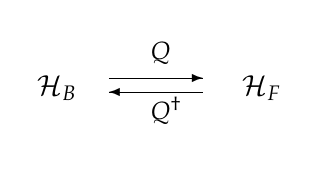
\begin{tikzpicture}
\node at (0.2,0) {$\calH_B$};
\node at (1.5,0) {$\raisebox{.6cm}{\maplr{Q}{Q^\dag}}$};
\node at (2.8,0) {$\calH_F$};
\end{tikzpicture}~.
$$
The Hamiltonian of a superymmstric theory is written as the anti-commutator of supercharges
$$
H:=\{Q,Q^{\dag}\}={ 1\over 2}\left(- {d^2 \over dx^2 }
+ W^\prime(x)^2\right) + {1 \over {2}}\sigma_3W^{\prime\prime}(x)
$$
 In other words, the supercharge is a ``square-root'' of Hamiltonian. In addition one can check that the supercharges commute with the Hamiltonian
\begin{equation}
[H,Q] =[H,Q^{\dag}] = 0 ~. 
\label{susyalg}
 \end{equation}
 
 Let us consider a bosonic eigenstate $|b\rangle \in\calH_B$ of the Hamiltonian
 $$ H |b\rangle =\{Q Q^\dag+Q^\dag Q\}|b\rangle =Q^\dag Q|b\rangle =E|b\rangle~, $$
 for $E>0$. Now its \textbf{superpartner} $|f\rangle =Q|b\rangle$ has  the same energy
 $$  H |f\rangle =\{Q Q^\dag+Q^\dag Q\}Q |b\rangle =Q Q^\dag Q|b\rangle =E|f\rangle~.$$
In a similar fashion, for a fermionic eigenstate $|f\rangle \in\calH_F$ with $E>0$, one can show that its superpartner $|b\rangle =Q^\dag|f\rangle$ has the same energy. In fact, the commutation relation \eqref{susyalg} is
responsible for the degeneracy.


\begin{figure}[h]\centering
\includegraphics{hilbert}
\end{figure}


On the other hands, situation drastically changes for states with $E=0$. For a  bosonic state $|b\rangle$ with zero energy $H|b\rangle=0$, we have $\langle b|Q^\dag Q |b\rangle=0$ so that the supercharge annihilates the state $Q|b\rangle=0$ and therefore there is no fermonic partner. Similarly, for a fermionic state $|f\rangle$, one can show that $Q^\dag |f\rangle$ so that there is no bosonic partner. Since  these zero energy states $|z\rangle$ are annihilated by both supercharges $Q$ and $Q^\dag$, they are invariant under supersymmetric transformation
$$
\exp(i\epsilon Q)|z\rangle=|z\rangle~,\qquad \exp(i\epsilon Q^\dag)|z\rangle=|z\rangle~.
$$
Therefore, they are also called \textbf{supersymmetric states}.



Witten considered the difference between bosonic and fermionic zero energy states \cite{Witten:1982}. To this end, he has introduced the index $\Tr(-1)^F$. Since the excited states do not contribute to the index because there are always boson-fermion pairs. Therefore, the index is equal to
$$
\Tr(-1)^F =\dim \Ker Q- \dim \Ker Q^\dag
$$
Note that the space of bosonic zero energy states can be expressed as $\Ker Q$ whereas the space of fermionic zero energy states can be written as $\Ker Q^\dag$.

Since zero energy sates obey
$$
\left(\frac{d}{dx}\pm W^\prime(x)\right)\phi(x)=0~,
$$
we have
$$
\phi(x)=\textrm{const} \times \exp(\mp W(x))~.
$$
The normalizability condition \eqref{L2} requires $\phi(x)\to 0$ as $|x|\to\infty$.   Suppose that the superpotential $W(x)$ is subject to polynomial growth $W(x)\sim \lambda x^n$ in the region $|x|\gg R$.

\begin{itemize}
\item When $n$ is even, there exists either bosonic or fermionic zero energy states depending on the sign of $\lambda$. Therefore, the index is equal to the sign of $\lambda$.
\item When $n$ is odd, there is no zero energy state because $W(x)$ changes the sign when $x$ moves from $-\infty$ to $\infty$ so that the index is equal to zero. Although the Hamiltonian is supersymmetric, there is no supersymmetric state for a potential of this type. Therefore, supersymmetry is \textbf{spontaneously broken}.
\end{itemize}

As we have seen, the index is independent of the detail of the superpotential $W(x)$ and it depends only on its asymptotic behavior. This is what we have seen in the first lecture.

%
%If $M$ is an even-dimensional,  oriented, spin-manifold with
%spin-bundles $S^{\pm}$ and
%$W$ is a vector bundle with unitary connection $A$ then the
%{\em coupled Dirac operator} is a natural first-order differential operator
%\begin{equation}
%\label{eq:dirac}
%D_A^+ \colon C^\infty(M, E^+) \to C^\infty(M, E^-).
%\end{equation}
%where
%\begin{equation} \label{1.27.9}
%E^+:=  S^+\otimes W,\;\;  E^-:= S^-\otimes W.
%\end{equation}
%If $M$ is compact, the Atiyah-Singer index theorem \cite{AS0, AS1} 
%gives a topological
%formula for the index of $D^+_A$,
%\begin{equation}
%\label{eq:indextheorem}
%\textrm{ind}(D^+_A):= \dim \ker (D^+_A)  - \dim \coker (D^+_A) = 
%\langle \hat A (M) \ch(W),  [M] \rangle.
%\end{equation}
%
%If $M$ is not a spin-manifold, `generalized Dirac operators' can be
%introduced, even though the Dirac operator itself is not
%well-defined. This can be done by observing that $E = E^+\oplus E^-$
%is a {\em Clifford module} (Clifford multiplication is extended to act
%as the identity on $W$) so that a compatible connection on $E$ leads
%to a Dirac operator as before.  If $M$ is not spin, there is an index
%theorem for Dirac operators defined on (hermitian) Clifford modules $E$
%which can be expressed in the form \cite{BerGetVer}
%\begin{equation} \label{eq:2.27.8}
%\ind(D^+_A) = \langle \widehat{A}(M)\ch(W), [M]\rangle
%\end{equation}
%where the notation will be explained below.  The definition is such
%that if $M$ is spin and \eqref{1.27.9} holds, then the {\em relative
%Chern character} $\ch(E/S)$ reduces to $\ch(W)$, the Chern character
%of $W$.
%
%
%
%
%
%\subsection{Clifford modules and Dirac operators}
%
%
%In the first part of this section we briefly recall the definitions and some basic
%facts about Clifford modules and Dirac operators. We refer the reader to
%\cite{BeGeVe,Duis96,LawMic89} for details. In our exposition we adopt the notations of
%\cite{BeGeVe}.
%
%In the second part of the section we present some examples of Clifford modules, which
%will be used in the subsequent sections.
%
%%---------------------------------------
%\subsubsection{The Clifford bundle}
%Suppose $(M,g)$ is an oriented Riemannian manifold of dimension $2n$. For any
%$x\in M$, we denote by $C(T^*_xM)=C^+(T^*_xM)\oplus C^-(T^*_xM)$ the Clifford
%algebra of the cotangent space $T_x^*M$, cf. \cite[\S3.3]{BeGeVe}.
%
%The {\em Clifford bundle \/} $C(M)$ of $M$ (cf. \cite[\S3.3]{BeGeVe}) is the
%$\ZZ_2$-graded bundle over $M$, whose fiber at $x\in M$ is $C(T^*_xM)$.
%
%
%The Riemannian metric $g$ induces the Levi-Civita connection $\nabla$ on $C(M)$
%which is compatible with the multiplication and preserves the $\ZZ_2$-grading on
%$C(M)$.
%
%%-----------------
%\subsubsection{Clifford modules}
%A {\em Clifford module \/} on $M$ is a complex vector bundle $\E$ on $M$ endowed
%with an action of the bundle $C(M)$. We write this action as
%%\[
%%        (a,s) \ \mapsto \ c(a)s, \quad \mbox{where} \quad
%%                        a\in \gc, \ s\in \gme.
%%\]
%
%A Clifford module $\E$ is called {\em self-adjoint \/} if it is endowed with a
%Hermitian metric such that the operator $c(v):\E_x\to\E_x$ is skew-adjoint, for
%any $x\in M$ and any $v\in T_x^*M$.
%
%
%A connection $\nabla^\E$ on a Clifford module $\E$ is called a {\em Clifford
%connection \/} if it is {\em compatible with the Clifford action}, i.e., if for
%any $a\in \gc$ and $X\in\Gamma(M,TM)$,
%\[
%        [\n^\E_X,c(a)] \ = \ c(\n_X a).
%\]
%In this formula, $\n_X$ is the Levi-Civita covariant derivative on $C(M)$, and
%$[\n^\E_X,c(a)]$ denotes the commutator of the operators $\n_X^\E$ and $c(a)$.
%
%
%Suppose $\E$ is a Clifford module and $\calW$ is a vector bundle over $M$. The
%{\em twisted Clifford module obtained from $\E$ by twisting with $\calW$ \/} is
%the bundle $\E\otimes\calW$ with Clifford action $c(a)\otimes1$. Note that the
%twisted Clifford module $\E\otimes\calW$ is self-adjoint if and only if so is
%$\E$.
%
%Let $\n^\calW$ be a connection on $\calW$ and let $\n^\E$ be a Clifford
%connection on $\E$. Then the {\em product connection}
%\begin{equation}\label{E:nEW}
%        \n^{\E\otimes\calW} \ = \ \n^\E\otimes 1 \ + \ 1\otimes \n^\calW
%\end{equation}
%is a Clifford connection on $\E\otimes\calW$.
%
%%------------------------
%\subsubsection{The chirality operator. The natural grading}
%Let $e_1\nek e_{2n}$ be an oriented orthonormal basis of $C(T_x^*M)$ and
%consider the element
%\begin{equation}\label{E:Gam}
%        \Gamma\ = \ i^n\, e_1\cdots e_{2n} \ \in \ C(T_x^*M)\otimes\CC.
%\end{equation}
%This element is independent of the choice of the basis, anti-commutes with any
%$v\in T_x^*M\subset C(T_x^*M)$, and satisfies $\Gamma^2=-1$, cf.
%\cite[\S3.2]{BeGeVe}. This element $\Gam$ is called the {\em chirality
%operator}. We also denote by $\Gam$ the section of $C(M)$ whose restriction to
%each fiber is equal to the chirality operator.
%
%Let $\E$ be a Clifford module, i.e. (cf. \eqref{clmodule}), a vector bundle over
%$M$ endowed with a fiberwise action of $C(M)$. Set
%\begin{equation}\label{E:grad}
%        \E^\pm \ = \ \{v\in \E: \ \Gam\, v=\pm v\}.
%\end{equation}
%Then $\E=\E^+\oplus\E^-$ is a {\em graded module} over $C(M)$ in the sense that
%$C^+(M)\cdot\E^\pm\subset \E^\pm$ and $C^-(M)\cdot\E^\pm\subset \E^\mp$.
%
%We refer to the grading \eqref{grad} as the {\em natural grading \/} on $\E$.
%Note that this grading is preserved by any Clifford connection on $\E$. Also, if
%$\E$ is a self-adjoint Clifford module (cf. \eqref{clmodule}), then the
%chirality operator $\Gam:\E\to\E$ is self-adjoint. Hence, the subbundles
%$\E^\pm$ are orthogonal with respect to the Hermitian metric on $\E$. {\em In
%this paper we endow all our Clifford modules with the natural grading.}
%
%
%
%
%
%
%
%%-------------------------------
%\subsubsection{Dirac operators}
%The {\em Dirac operator \/} associated to a Clifford connection $\n^\E$ is
%defined by the following composition
%%\begin{equation}\label{E:dir1}
%%\begin{CD}
%%        \gme @>\n^\E>> \g(M,T^*M\otimes \E) @>c>> \gme.
%%\end{CD}
%%\end{equation}
%In local coordinates, this operator may be written as $D=\sum\,
%c(dx^i)\,\n^\E$. Note that $D$ sends even sections to odd sections and
%vice versa: $D:\, \Gam(M,\E^\pm)\to \Gam(M,\E^\mp)$.
%
%Suppose that the Clifford module $\E$ is endowed with a Hermitian structure and
%consider the $L_2$-scalar product on the space of sections  defined by the
%Riemannian metric on $M$ and the Hermitian structure on $\E$. By
%\cite[Proposition~3.44]{BeGeVe}, {\em the Dirac operator associated to a
%Clifford connection $\n^\E$ is formally self-adjoint with respect to this scalar
%product if and only if $\E$ is a self-adjoint Clifford module and $\n^\E$ is a
%Hermitian connection.}


\section{Epilogue: quantum Hall effects \cite{Witten:2015}}
This section is essentially a write-up of Witten's slides \cite{Witten:2005}.


\subsection{What is the Hall effect?}

\begin{figure}[h]\centering
\includegraphics[width=3cm]{E}
\end{figure}

 An electron in an electric field is accelerated
$$
m\frac{d^2\vec{x}}{dt^2} =e\vec{E} \quad \longrightarrow \quad  \vec{v}=\frac{d\vec{x}}{dt} \sim \frac{e\vec{E}}{m}t
$$
   If the electron is in an obstacle course  which randomizes its velocity on an average after a time $\tau$, then the velocity will not go to infinity, but to 
   $$
   \langle \vec{v}\rangle \sim  \frac{e\vec{E}}{m}\frac{\tau}{2}
   $$
 It $\cN$ is the number density of electrons that are free to move, The average current will be  be roughly 
$$ 
\vec{J}=\cN e \langle \vec{v}\rangle=\frac{\cN e^2\tau }{2m}\vec{E}\quad \longrightarrow \quad \vec{J}=\sigma\vec{E}
$$
where  the conductivity is $\sigma=\frac{\cN e^2\tau}{2m}$ in this approximation. (No topology here - $\sigma$ depends on all the details.) Now in a magnetic field $\vec{B}$ 
$$
m\frac{d^2\vec{x}}{dt^2} =\frac{e}{c}\frac{d\vec{x}}{dt}\times \vec{B}
$$
\begin{figure}[h]\centering
\includegraphics[width=5cm]{B}
\end{figure}
 The electron motion is spiral. Uniform motion along $\vec{B}$ and circular oscillations normal to $\vec{B}$. To get the Hall effect. we want to combine perpendicular $\vec{E}$ and $\vec{B}$  with $\vec{E}\ll\vec{B}$. The electron now drifts out at the page, with velocity 
 $$
\vec{v} = c \frac{\vec{E}\times\vec{B}}{|\vec{B}|^2}
$$

\begin{figure}[h]\centering
\includegraphics[width=10cm]{EB}
\end{figure}
With no magnetic field, the current $\vec{J}$ is in the $\vec{E}$ direction, but with a strong magnetic field, the current flow is perpendicular to $\vec E$ and $\vec B$. With average velocity $\vec{v} = c \frac{\vec{E}\times\vec{B}}{|\vec{B}|^2}
$ for each electron, the current is
$$
\vec{J}=\cN e \vec{v}=\cN e c \frac{\vec{E}\times\vec{B}}{|\vec{B}|^2}=\sigma_H \widehat{B}\times \vec{E}
$$
where $ \widehat{B}=\vec{B}/|\vec{B}|$ the Hall conductivity is $\sigma_H=\cN e c/|\vec{B}|$. (no topology here!)

\subsection{What is the quantum Hall effect?}
The quantum Hall effect arises if we consider a very thin sample: special composition, low temperature, large $\vec B$ which effectively is a 2d surface - a molecular monolayer. Here we find, for certain type of material, in certain ranges of $\vec B$ and temperature, that the Hall conductivity does have a magic value 
$$
\sigma_H=\frac{e^2}{\hbar} n \qquad n\in\bZ
$$
where $\hbar$ is the Planck courant. This value is unchanged as $\vec B$, temperature, chemical composition impurity concentration, etc. are varied  within certain limits.

\begin{figure}[h]\centering
\includegraphics[width=8cm]{integer}
\end{figure}


The integrality of $\frac{\hbar}{e^2}\sigma_H$, is verified so precisely that it has become the most accurate way to measure $\frac{e^2}{\hbar}$. There is an integer here, so we should seek a topological explanation! But how can we hope to find one in the messy world of condensed mater physics? In this measurement, we are looking at very large samples observed for very long times, compared to atomic distance and times. One of the main reasons that it is possible in physics is that in any observation made at a certain scale of length and time. Most of microscopic degree of freedom - needed for a much shorter lengths and times - are irrelevant. This notion of \textbf{effective theory} is called \textbf{universality}.


Familiar example is a rigid body: The only relevant degree of freedom is the time-dependent embedding in space.

Solids vary widely in their relevant degrees of freedom:
\begin{itemize}
\item vibrations are always relevant for certain questions, but not for electromagnetic behavior like the Hall effect
\item electrons are relevant in conductors where they are free to move, but not in insulators.
\item an exotic example of a relevant variable is the trivialization $s$ of the line bundle $\cL^2$ in a superconductor
\item another exotic example arises in the ``fractional quantum Hall effect'', when $\sigma_H\frac{\hbar}{e^2}$ is a rational number not an integer.
\end{itemize}


Whatever the relevant degrees of freedom may be in a particular case, the macroscopic interactions of electromagnetism with the solid are described by Euler-Lagrange equation and quantization from an action 
$$
L=L_{\textrm{vacuum}}+L_{\textrm{solid}}~.
$$
Here $L_{\textrm{vacuum}}$ is the Lagrangian in vacuum of the electromagnetic field. If $A$ is $U(1)$ connection  and $F=dA$ is the curvature, then 
$$
L_{\textrm{vacuum}}=\frac{\hbar}{4e^2}\int _{\mathbb{R}^{3,1}}F\wedge \ast F~.
$$
The part of the action due to the solid is 
$$
L_{\textrm{solid}}=\int _{\textrm{solid}\times \textrm{time}}d\mu~ W\left( \Phi ,A\right)~,
$$
where $W$ is a local functional of the relevant  degrees of freedom $\Phi$ as well as the connection $A$. ``Locality'' means that the variation of $W$ is a gauge -invariant differential polynomial in $\Phi$, $A$. The total action is thus
$$
\dfrac {\hbar}{4e^{2}}\int _{\mathbb{R}^{3 ,1}}F\wedge \ast F+\int _{\textrm{solid}}d\mu~ W\left( \Phi ,A\right)~.
$$
The Euler-Lagrange equation for $A$ becomes
$$
d\left( \ast F\right) =-\dfrac {e^{2}}{\hbar}\dfrac {\delta W}{\delta A}\left( \Phi ,A\right)
$$
and if we compare to freshman physics
$$
\ast d(\ast F)=4\pi J 
$$
Now what are the relevant degrees of freedom for the quantum Hall effect? (Answer: for the ordinary integer quantum Hall effect, there are none.) Materials with no relevant degrees of freedom in their interaction with electromagnetism are not unusual. (An ordinary pane of class is an example.) It means that $W(\Phi,A)$ reduces to $W(A)$.


\subsection{Some condensed matter physics}

Before trying to discuss the quantum Hall effect, let us discuss a 3-dimensional piece of class. So we will feel to know what we are doing. The local structure is invariant under rotations and reflections, which will constrain $W$. A drastic simplification comes from the following. Grade the monomials in $W$ by ``dimension''
$$
\dim A=1 ~,\qquad  \dim \frac\partial{\partial x}=\dim \frac\partial{\partial t}=1~, \qquad \dim \vec E=\dim \vec B=2~.
$$
If all fields and frequencies are small on an atomic scale, terms of higher dimension are smaller. This is essentially always true in practice, and anyway otherwise the effective description is not valid. The vacuum part of the action 
$$
L_{\textrm{vacuum}}=\frac{\hbar}{4e^2}\int _{\mathbb{R}^{3,1}}F\wedge \ast F~.
$$
is of dimension four, so we can neglect in $W(A)$ terms of dimension greater than four. Using rotation invariance and reflection symmetry, $W(A)$ cannot have any terms linear in $\vec E$ or $\vec B$ so the lowest dimension terms are 
$$
W(A)=\int d^4x(\epsilon \vec E^2-\mu \vec B^2)
$$
where $\epsilon$ and $\mu$ are the electric and magnetic susceptibilities. To find how glass interacts with electromagnetism, we just look at the combined Lagrangian
$$
\frac{\hbar}{4e^2}\int _{\mathbb{R}^{3,1}}F\wedge \ast F+\int d^4x(\epsilon \vec E^2-\mu \vec B^2)=\int d^4x\Big(\Big(\frac{\hbar}{4e^2}+\epsilon\Big) \vec E^2-\Big(\frac{\hbar}{4e^2}+\mu\Big)  \vec B^2\Big)~.
$$
The resulting Euler-Langrange equations are Maxwell's equations, but with a reduced speed of light. 

If instead of glass, we consider a crystal (still with no relevant degrees of freedom), then $W$ can have general quadratic terms in $\vec E$ and $\vec B$
$$
\int d^4x(\epsilon_{ij} E_i E_j-\mu_{ij} B_i B_j)~.
$$
We get an anisotropic speed of light and ``birefringence''. If the crystal lacks reflection symmetry, then $W(A)$ can contain terms linear in $\vec E$ and $\vec B$
$$
\Delta W=\int d^4x (\vec n\cdot \vec E+\vec m\cdot \vec B)
$$
where $\vec n$ and $\vec m$ depend on the crystal axes. Such materials are ``ferroelectric'' and ``ferromagnetic'', as one can learn by deriving and solving the Euler-Lagrange equations. By now we know how to study materials with no relevant degrees of freedom: \textbf{write the possible terms in $W(A)$ of low dimension. derive and solve the Euler-Lagrange equations.} The hypothesis that there are no relevant degrees of freedom ensures that $W(A)$ is a local functional of $A$ only.


\subsection{Some geometry}


Now we are ready to study the quantum Hall effect, which involves an atomic monolayer or a 2d surface in space. Hence, the spacetime sweeps out a three-manifold $Q=\Sigma\times \bR$ where $\bR$ parametrizes time. So we are doing $U(1)$ gauge theory on a three-manifold $Q$, and the reason that we will get something interesting is that there is an unusual term, of topological interest, that can appear in $Q(A)$. This is the Chern-Simons form. We can assume that $Q$ is the boundary of a 4-manifold $M$ over which the electromagnetic line bundle $\cL$ and connection $A$ extend and we write 
$$
S_M(A)=\frac{1}{4\pi^2}\int_M F\wedge F
$$
This depends on $M$, but only slightly
$$
S_M(A)-S_{M'}(A)=\frac{1}{4\pi^2}\int_X F\wedge F\in \bZ
$$
\begin{figure}[h]\centering
\includegraphics[width=9cm]{4d-3d}
\end{figure}

So as a map to $\bR/\bZ$, $S_M(A)$ is independent of $M$ and we just call it $S(A)$. Concretely, for a trivial line bundle $\cL$, we have $$S(A)=\frac{1}{4\pi^2}\int_Q A\wedge dA~.$$
$S(A)$ has a low dimension -three- so if we can include it in $W(A)$, the effective action, then this will be important? Does it make sense to do this, given that $S(A)$ has an additive integer indeterminacy?

In classical mechanics, adding a constant to the action $I$ does not matter as it does not affect the Euler-Lagrange equation. In quantization, one needs to be able to define $\exp(iI)$. To compute quantum transition amplitude, so I can have an additive ambiguity, but this must be of the form $2\pi k$ for $k\in \bZ$. So a conceivable material may have in the electromagnetic effective action $W(A)$ a multiple of $S(A)$, but it must be a very special multiple:
$$
W(A)=2\pi k S(A)=\frac{k}{2\pi}\int A\wedge dA~,
$$
for some $k\in \bZ$ (which depends on the material, the magnetic field, etc.) 



%
%\subsection{ The Jones polynomial}
%
%This also works in the non-Abelian case 
%. $A$ is the connection on a $G$-bundle for compact simple $G$ over 3-manifold $Q$ and the action
%$$
%W(A)=\frac{k}{2\pi}\int_Q \textrm{Tr}(A\wedge dA+\frac23A\wedge A\wedge A)
%$$
%where $W$ maps to $\bR/2\pi \bZ$. So we can consider a quantum theory in which $W(A)$ is the complete action. The quantum path integral on a 3-manifold $Q$ is formally
%$$
%Z(M)=\int_{\cA/\cG}\cD A\exp(iW(A))
%$$
%where $\cA$ is the space of connections and $\cG$ is the gauge transformation $\textrm{Map}(Q,G)$. This is the quantum 3-manifold invariant with $q=e^{2\pi i /(k+h)}$. The same theory also leads to the Jones polynomial of knots and its generalizations. 
%$$
%\Phi _{R}\left( C\right) =\dfrac {1}{Z\left( M\right) }\int _{\cA/\cG}\cD A\exp iW\left( A\right) \mathrm{Tr}_{R}Hol\left( A;C\right)
%$$
%When the gauge group is Abelian, one still gets knot and 3-manifold invariants. But they are ``classical'' ones; linking numbers, torsion, eta-invariant. 



\subsection{Theory of the quantum Hall effect}


Now let us go back to the quantum Hall effect where the gauge group (for the class of materials we are considering) is Abelian. We consider a flat sample in the x-y plane with $k\neq 0$.
$$
L=\frac{\hbar}{4e^2}\int_{\bR^{1,3}} F\wedge \ast F +\frac{k}{2\pi}\int_{\textrm{sample}\times \textrm{time}} A\wedge dA
$$
The electromagnetic current is 
$$
J=\frac{4\pi e^2}{\hbar}\frac{\delta W}{\delta A}=\frac{e^2k}{\hbar} (\ast_3 F)
$$
where $\ast_3$ is the Hodge star in the 3-dimensional spacetime for the sample. In a non-relativistic Language, this becomes 
$$
J_x=\frac{e^2k}{\hbar} E_y ~,\qquad J_y=-\frac{e^2k}{\hbar} E_x ~.
$$
We have found the quantum Hall effect $\sigma_H=\frac{e^2}{\hbar}k$. 
\begin{figure}[h]\centering
\includegraphics[width=5cm]{plane}
\end{figure}

For fractional quantum Hall effects, we add a new $U(1)'$ gauge field $B$ with the old $U(1)$ gauge field $A$
$$
\frac{\hbar}{4e^2}\int F\wedge \ast F +\frac{k_1}{2\pi}\int A\wedge dA+\frac{k_2}{\pi}\int A\wedge dB+\frac{k_3}{2\pi}\int B\wedge dB~.
$$
where $B$ can be interpreted as an ``emergent'' gauge field that only propagates in the sample.
By integrating out $B$ field, one can check that the conductivity becomes fractional $$\sigma_H=\frac{e^2}{\hbar}\left(k_1-\frac{k_2^2}{k_3}\right)~.$$




\section{Extra Lecture 1: \cite{Nakahara} \S 8}


\subsection{Complex manifolds}


\begin{defn}[Complex manifold]\index{Complex Manifold}
Let $M$ be an $2n$-dimensional manifold. $M$ is a \textbf{complex manifold} of complex dimension $n$ if 
  \begin{enumerate}
    \item Let $M = \bigcup_{\alpha} U_\alpha$ be an open covering.
    \item   There is a homeomorphism $\varphi_\alpha: U_\alpha \to \varphi_\alpha(U_\alpha) \subseteq \C^n$, where $\varphi(U_\alpha)$ is open in $\C^n$.
    \item For all $\alpha, \beta$, we have $\varphi_\alpha(U_\alpha \cap U_\beta)$ is open in $\C^n$, and the transition function
      \[
        \varphi_\alpha \circ \varphi_\beta^{-1}: \varphi_\beta(U_\alpha \cap U_\beta) \to \varphi_\alpha(U_\alpha \cap U_\beta)
      \]
      is holomorphic (i.e. they depend only on the $z_{\mu}$ but not on their complex conjugate).
  \end{enumerate}
\end{defn}
\begin{center}
  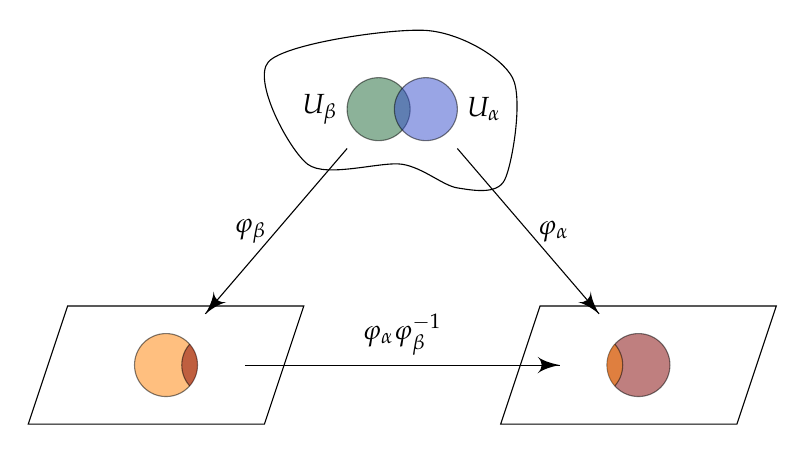
\begin{tikzpicture}
    \draw plot [smooth cycle] coordinates {(-1.2, -0.7) (0, -0.7) (0.7, -1) (1.3, -0.9) (1.4, 0.4) (0.3, 1) (-1.7, 0.6)};

    \draw (-0.3, 0) [fill=mgreen, opacity=0.5] circle [radius=0.4];
    \draw (0.3, 0) [fill=mblue, opacity=0.5] circle [radius=0.4];

    \node [left] at (-0.7, 0) {$U_\beta$};
    \node [right] at (0.7, 0) {$U_\alpha$};

    \begin{scope}[shift={(-4.75, -4)}]
      \draw (0, 0) -- (3, 0) -- (3.5, 1.5) -- (0.5, 1.5) -- cycle;

      \draw (1.75, 0.75) [fill=morange, opacity=0.5] circle [radius=0.4];
      \begin{scope}
        \clip (1.75, 0.75) circle [radius=0.4];
        \draw (2.35, 0.75) [fill=mred, opacity=0.5] circle [radius=0.4];
      \end{scope}
    \end{scope}

    \draw [->] (-0.7, -0.5) -- (-2.5, -2.6) node [pos=0.5, left] {$\varphi_\beta$};
    \draw [->] (0.7, -0.5) -- (2.5, -2.6) node [pos=0.5, right] {$\varphi_\alpha$};

    \begin{scope}[shift={(1.25, -4)}]
      \draw (0, 0) -- (3, 0) -- (3.5, 1.5) -- (0.5, 1.5) -- cycle;

      \draw (1.75, 0.75) [fill=mred, opacity=0.5] circle [radius=0.4];
      \begin{scope}
        \clip (1.75, 0.75) circle [radius=0.4];
        \draw (1.15, 0.75) [fill=morange, opacity=0.5] circle [radius=0.4];
      \end{scope}
    \end{scope}
    \draw [->] (-2, -3.25) -- (2, -3.25) node [pos=0.5, above] {$\varphi_\alpha \varphi_\beta^{-1}$};
  \end{tikzpicture}
\end{center}

As we consider differentiable (smooth) maps between two smooth manifolds $M$ and $N$, we can consider holomorphic maps between two complex manifolds $M$ and $N$. Let $M$ and $N$  be smooth manifolds, and let $\{(U_\alpha, \varphi_\alpha)\}_\alpha$ and $\{(V_\beta, \psi_\beta)\}_\beta$ be their  atlas. 

\begin{defn}[holomorphic map]\index{holomorphic map}
  A map $f: M \to N$ is \textbf{holomorphic} if, for a chart $(U_\alpha, \varphi_\alpha)$ of $p\in M$ and $(V_\beta, \psi_\beta)$ of $f(p)\in N$,  $ \psi_\beta \circ f \circ ( \varphi_\alpha)^{-1}: \varphi(U_\alpha \cap f^{-1} (V_\beta)) \to \xi(V_\beta )$ is holomorphic.


If there is the inverse map that is holomorphic, it is called a \term{biholomorphic} map, or $M$ and $N$ are \term{biholomorphic equivalent}.

\end{defn}
\begin{center}
  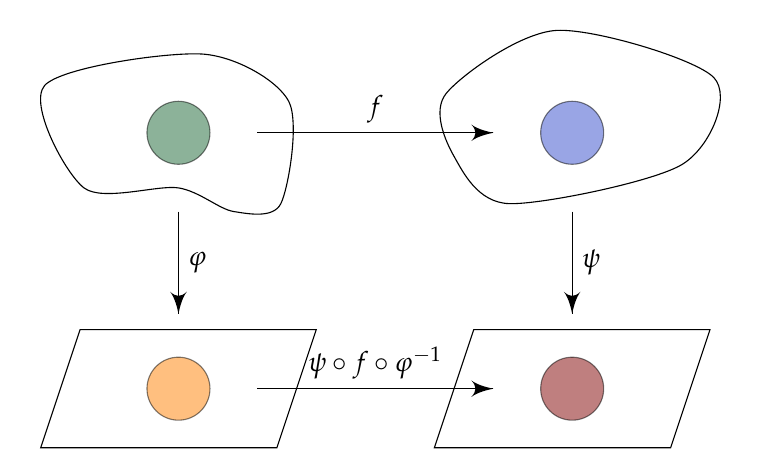
\begin{tikzpicture}
    \draw plot [smooth cycle] coordinates {(-1.2, -0.7) (0, -0.7) (0.7, -1) (1.3, -0.9) (1.4, 0.4) (0.3, 1) (-1.7, 0.6)};

    \draw [fill=mgreen, opacity=0.5] circle [radius=0.4];

    \begin{scope}[shift={(-1.75, -4)}]
      \draw (0, 0) -- (3, 0) -- (3.5, 1.5) -- (0.5, 1.5) -- cycle;

      \draw (1.75, 0.75) [fill=morange, opacity=0.5] circle [radius=0.4];
    \end{scope}

    \draw [->] (0, -1) -- +(0, -1.3) node [pos=0.5, right] {$\varphi$};
    \begin{scope}[shift={(5, 0)}]
      \draw plot [smooth cycle] coordinates {(1.4, -0.4) (-0.8, -0.9) (-1.5, -0.3) (-1.6, 0.5) (-0.2, 1.3) (1.8, 0.7)};

      \draw [fill=mblue, opacity=0.5] circle [radius=0.4];

      \begin{scope}[shift={(-1.75, -4)}]
        \draw (0, 0) -- (3, 0) -- (3.5, 1.5) -- (0.5, 1.5) -- cycle;

        \draw (1.75, 0.75) [fill=mred, opacity=0.5] circle [radius=0.4];
      \end{scope}

      \draw [->] (0, -1) -- +(0, -1.3) node [pos=0.5, right] {$\psi$};
    \end{scope}

    \draw [->] (1, 0) -- (4, 0) node [above, pos=0.5] {$f$};

    \draw [->] (1, -3.25) -- (4, -3.25) node [above, pos=0.5] {$\psi \circ f \circ \varphi^{-1}$};
  \end{tikzpicture}
\end{center}




\begin{example}
Complex projective space $\CP^n$ is a complex manifold. (Check it satisfies the definition.)
\end{example}



\begin{example}
Let us now consider compact complex manifolds. It turns out that submanifolds of $\C^n$ are not  interesting, since a connected compact analytic submanifold of $\C^n$ is a point. However, many compact complex manifolds can be constructed as submanifolds of projective spaces $\CP^n$. We saw that $\CP^n$ is compact; all its closed complex submanifolds are also compact. In fact, there is a theorem by Chow stating that any compact submanifold of $\CP^n$ can be realized as the zero loci $F_i(z)=0$ of a finite number of homogeneous polynomial equations in the homogeneous coordinates $z_{\mu}$. These compact complex manifolds are called  \term{complex projective variety}. One important example is the \term{Fermat quintic} in $\CP^4$, given as the zero locus of the equation
\be
5\psi z_0z_1z_2z_3z_4-\sum_{\mu=0}^4 (z_{\mu})^5 = 0.
\ee
This three-dimensional compact complex manifold turns out to be \CY, probably the most studied \CY\ threefold because of mirror symmetry \cite{Candelas}. 
\end{example}



\subsection{Holomorphic vector bundles}


\begin{defn}[Holomorphic vector bundle]\index{vector bundle}
  Let $M$ be a complex manifold and let $\pi: E \to M$ be a vector bundle of real rank $2r$
  \begin{enumerate}
    \item For each $p \in M$, the fiber $\pi^{-1}(p) = E_p$ is an $r$-dimensional complex vector space,
    \item For all $p \in M$, there is an open $U \subseteq M$ containing $p$ and a diffeomorphism
      \[
        t: E_U = \pi^{-1}(U) \to U \times \C^r
      \]
      such that
      \[
        \begin{tikzcd}
          E_U \ar[r, "t"] \ar[d, "\pi"] & U \times \C^r \ar[dl, "p_1"]\\
          U
        \end{tikzcd}
      \]
      commutes, and the induced map $E_q \to \{q\} \times \C^r$ is a linear isomorphism for all $q \in U$.
     \item 
  Suppose that $t_\alpha: E|_{U_\alpha} \to U_\alpha \times \C^r$ and $t_\beta: E|_{U_\beta} \to U_\beta \times \C^r$ are trivializations of $E$. Then
  \[
    t_\alpha \circ t_\beta^{-1} : (U_\alpha \cap U_\beta) \times \C^r \to (U_\alpha \cap U_\beta) \times \C^r
  \]
  is fiberwise linear, i.e.
  \[
    t_\alpha \circ t_\beta^{-1}(q, v) = (q, g_{\alpha\beta}(z) v),
  \]
  where $g_{\alpha\beta}(z):U_\alpha \cap U_\beta\to \GL(r,\C)$ is a holomorphic function.
The transition functions have the following properties
  \begin{enumerate}
    \item $g_{\alpha\alpha} = \id$
    \item $g_{\alpha\beta} = g_{\beta\alpha}^{-1}$
    \item $g_{\alpha\beta}g_{\beta\gamma} g_{\gamma\alpha}= 1$.
  \end{enumerate}
  \end{enumerate}
\end{defn}


\subsubsection{Holomorphic tangent and cotangent bundle}
Let $(U,(z_1,\cdots,z_n))$ be a local coordinate of a complex manifold $M$ and we decompose the complex coordinate $z_j=x_j+iy_j$ into the real and imaginary part. Then, the basis of the tangent bundle $TM$ on an open set $U\subset M$ can be taken by $\frac\partial{\partial x_j}$, $\frac\partial{\partial y_j}$ ($j=1,\cdots,n$). Now let us complexify the tangent bundle $T_{\C} M:=TM\otimes \bC$ where we can take the basis on $U$ as
$$
\frac\partial{\partial z_j}:=\frac12\Big(\frac\partial{\partial x_j}-i\frac\partial{\partial y_j}\Big)~,\qquad \frac\partial{\partial \overline z_j}:=\frac12\Big(\frac\partial{\partial x_j}+i\frac\partial{\partial y_j}\Big)~.
$$
Each fiber of $T_pM\otimes \C$ is a vector space with basis  $\frac\partial{\partial x_j}$, $\frac\partial{\partial y_j}$ on $\C$. Similarly, one can complexify the cotangent bundle $T_{\C}^* M:=T^*M\otimes \C$ where we can take basis $dz_j$, $d\overline z_j$ on $U$. At each point $p\in M$, we can take the subspace $T^{(1,0)}_p M$ of $T_p M\otimes \C$ spanned by $\{\frac\partial{\partial z_j}\}$. A family of the subspace is denoted by $T^{(1,0)} M =\cup_p T^{(1,0)}_p M$ and we can also define $T^{*(1,0)} M =\cup_p T^{*(1,0)}_p M$ in a similar fashion. Given another chart $(V(w_1,\cdots,w_n))$, they transform 
$$
\frac\partial{\partial z_j}=\frac{\partial w_k}{\partial z_j}\frac\partial{\partial w_k}~, \quad dz_j=\frac{\partial z_j}{\partial w_k}dw_k
$$ 
where the transition functions $\frac{\partial w_k}{\partial z_j}$ and $\frac{\partial z_j}{\partial w_k}$ are holomorphic so that they are holomorphic vector bundles. Indeed, we can decompose complxified (co)tangent bundle as
$$T_{\C} M = T^{(1,0)} M \oplus T^{(0,1)} M~,\qquad T_{\C}^* M = T^{*(1,0)} M \oplus T^{*(0,1)} M~.$$
We call $T^{(1,0)} M$ (resp. $T^{(0,1)} M$) the \term{holomorphic (resp. anti-holomorphic) (co)tangent bundle}. 


As a real bundle. $T^{(1,0)} M$ is isomorphic to $T M$. In fact, We can define a map $\textrm{Re}:T_\C M\to TM$ by taking real part
$$
2\textrm{Re}~\frac\partial{\partial z_j}=\frac\partial{\partial x_j}~,
$$ 
 which is an isomorphism. Since $T^{(1,0)} M$ is a complex vector bundle, we have the multiplication by $i$, which induces an isomorphism $J:TM\to TM$:
 $$
 2\textrm{Re}~\frac\partial{\partial z_j}=\frac\partial{\partial x_j}~,\quad  2\textrm{Re}~ i\frac\partial{\partial z_j}=\frac\partial{\partial y_j}~,
 $$
 so that
 $$
 J\Big( \frac\partial{\partial x_j}\Big)= \frac\partial{\partial y_j}~,\quad  J\Big( \frac\partial{\partial y_j}\Big)= -\frac\partial{\partial x_j}~.
 $$
It is easy to check $J^2=-\textrm{id}_{TM}$, and  the eigenvalues of $J$ in $T_pM \otimes \C$ are $\pm i$. Hence, we consider $T^{(1,0)}_p M$ (resp. $T^{(0,1)}_p M$) as the eigenspace of $J_p$ with eigenvalue $i$ (resp. $-i$). $J$ is called \term{almost complex structure}.
 
 An almost complex structure $J_M:TM\to TM$ is a complex structure if for any $p\in m$ there exist an open neighborhood $p\in U\subset M$, $V\subset \C^n$, and a continuous map $\varphi:U\to V$ such that $d\varphi\cdot J_M=J_{\C^n}\cdot d\varphi$. If an almost complex structure $J_M$ is a complex structure, $J_M$ is called to be \term{integrable}. The Newlander-Nirenberg theorem states that an almost complex structure $J$ is integrable if and only if the Nijenhuis tensor vanishes:
 $$
 N_{J}(X,Y)=-J^{2}[X,Y]+J([JX,Y]+[X,JY])-[JX,JY]=0~$$
 for ${}^\forall X,Y\in \mathfrak{X}(M)$.
 
 
 The only spheres which admit almost complex structures are $S^2$ and $S^6$. In particular, $S^4$ cannot be given an almost complex structure. In the case of $S^2$, the almost complex structure comes from the complex structure of the Riemann sphere. The 6-sphere $S^6$ inherits an almost complex structure from the octonion multiplication;. However, whether $S^6$ has a complex structure is an open question.

\subsubsection{Differential forms}
Locally, any differential forms can be expressed as a linear combination of the exterior products of $dz_j$ and $d\overline z_k$. In particular, a differential form which can be expanded in terms of
$$
dz_{i_1}\wedge \cdots \wedge dz_{i_p}\wedge d\overline z_{i_1}\wedge \cdots \wedge d\overline z_{i_q}
$$
called $(p,q)$-form, which is a section of $\bigwedge^p T^{*(1,0)} M \otimes \bigwedge^{q} T^{*(0,1)} M$. We denote the vector space of $(p,q)$-forms by $\Omega^{p,q}(M)$.
In fact,  it is easy to show that the following complexified bundles decompose as
$$
\bigwedge^k T^*_{\C} M = \bigoplus_{j=0}^k \bigwedge^j T^{*(1,0)} M \otimes \bigwedge^{k-j} T^{*(0,1)} M,
$$

On a complex manifold, the exterior derivative also admits a simple decomposition: $d = \partial + \bar{\partial}$, where we defined the operators 
$$\partial: \Omega^{p,q}(M) \to \Omega^{p+1,q}(M)~,\qquad \bar{\partial}: \Omega^{p,q}(M) \to \Omega^{p,q+1}(M)~.$$
The identity $d^2=0$ implies that $\partial^2=\bar{\partial}^2=0$ and $\partial \bar{\partial}+\bar{\partial} \partial=0$. 
%We can also define a real operator $d^c: \Omega^k_{\C} (M) \to \Omega^{k+1}_{\C} (M)$ by $d^c = i (\bar{\partial}-\partial)$, which satisfies
%\be
%d d^c + d^c d=0,~~~(d^c)^2=0,~~~\partial = \frac12 (d+id^c),~~~\bar{\partial} = \frac12 (d-id^c),~~~d d^c = 2i \partial \bar{\partial}.
%\ee

A $(p,0)$-form is an element of $\Omega^{p,0}(M)$ and it can be locally written as
$$
\varphi=\sum \varphi_{i_1, \cdots  ,i_p}(z)dz_{i_1}\wedge \cdots \wedge dz_{i_p}
$$
where $\varphi_{i_1, \cdots  ,i_p}(z)$ is holomorphic. Therefore, $\phi$ is called \term{a holomorphic $p$-form}. In particular, when $p=n$, 
$$
K_M=\bigwedge^n  T^{*(1,0)} M
$$
is called \term{the canonical line bundle}. Since $TM$ is isomorphic to $ T^{(1,0)} M$, the first Chern class is
$$
c_1(M)=c_1(TM)=c_1(T^{(1,0)} M)=c_1(\bigwedge^n  T^{(1,0)} M)=-c_1(K_M)
$$


Now what is the analog of the de Rham cohomology groups for complex manifolds? 

\begin{defn}
Let $M$ be a complex manifold of complex dimension $m$. As $\bar{\partial}^2=0$, we can form the complex
$$
\begin{array}{ccccccccccc}
&\bar{\partial}&&\bar{\partial}&&\bar{\partial}&&\bar{\partial}&&\bar{\partial}&\\
0 &\to& \Omega^{p,0}(M) &\to& \Omega^{p,1}(M) &\to& \ldots &\to& \Omega^{p,n}(M) &\to&0.
\end{array}
$$
We define the \term{Dolbeault cohomology groups} $H^{p,q}_{\bar{\partial}} (M)$ of $M$ by
$$
H^{p,q}_{\bar{\partial}} (M) = {{\rm Ker}(\bar{\partial}: \Omega^{p,q}(M) \to \Omega^{p,q+1}(M)) \over {\rm Im} (\bar{\partial}: \Omega^{p,q-1}(M) \to \Omega^{p,q}(M))}.
$$
\end{defn}

Remark that the Dolbeault cohomology groups depend on the complex structure of $M$. Note also that we could have defined the cohomology groups using $\partial$ instead of $\bar{\partial}$, this is just a matter of convention since they are complex conjugate. 

\begin{thm}[Hodge decomposition theorem for K\"ahler manifolds]
For a compact K\"ahler manifold $M$, the complex cohomology satisfies
\begin{align}
H^r(M, \C) \cong \bigoplus_{p+q=r}H^{p,q}_{\bar{\partial}} (M) ~,\cr
H^{p,q}_{\bar{\partial}} (M) =\overline{H^{q,p}_{\bar{\partial}} (M)}
\end{align}
where $H^{p,q}_{\bar{\partial}} $
is the Dolbeault cohomology restricted to forms of type $(p, q)$. Further, we could
instead choose the de Rham cohomology to obtain the same result, and the cohomology classes
contain unique harmonic representatives. Consequently, holomorphic forms are therefore
harmonic for any K\"ahler  metric on a compact manifold, and the odd Betti numbers are
even.
\end{thm}


We now define the \term{Hodge numbers}  to be $h^{p,q} = \dim H^{p,q}_{\bar{\partial}} (M)$. The Hodge numbers of a complex manifold are summarized in what is commonly called the \term{Hodge diamond}:
$$
\begin{array}{ccccc}
&&h^{n,n}&& \\
&h^{n,n-1}&\vdots&h^{n-1,n}& \\
h^{n,0}&\cdots&&\cdots&h^{0,n}\\
&h^{1,0}&\vdots&h^{1,0}& \\
&&h^{0,0}&& \\
\end{array}
$$



\begin{thm}[Hard Lefschetz Theorem] Let $(M, \omega)$ be a K\'ahler manifold. Let $L$ be
exterior multiplication by the K\"ahler form $\omega$. Then
$$L^k: H^{n-k}(M) \to H^{n+k}(M)$$
is an isomorphism for $1 \le k \le n$. Further, if we define the primitive cohomology $P^j(M)$ by
$$P^j(M) = \ker L^{n-j+1} : H^j \to H^{2n-j+2}~,$$
then we have the Lefschetz decomposition
$$H^m (M) = \bigoplus_k L^k P^{m-2k}(M)~.$$
Thus, the Betti numbers of a compact K\"ahler manifold have a pyramid structure, called the
\term{Hodge pyramid}.
\end{thm}











\subsection{K\"ahler manifolds}

The condition for a Riemannian metric $g$ to be Hermitian is that for ${}^\forall X,Y\in \mathfrak{X}(M)$, and ${}^\forall \alpha,\beta\in\C$,  it satisfies
$$
g(\alpha X,\beta y)= \alpha \overline\beta g(X,Y)~.
$$
This condition amounts to the case when $\alpha=\beta=i$. Since the multiplication by $i$ corresponds to $J$, the Hermitian metric can be defined as follows.

\begin{defn}
Let $(M,J)$ be a complex manifold, and let $g$ be a Riemannian metric on $M$. We call $g$ a \term{Hermitian metric} if $g(v,w) = g(Jv,Jw)$ for all vector fields $v,w$ on $M$
%\item{In component notation, $g_{ab} = J_a^c J_b^d g_{cd}$;}
%\item{Using the greek indices notation, $g_{ab}=g_{\alpha \bar{\beta}}+g_{\bar{\alpha} \beta}$, that is $g_{\alpha \beta} = g_{\bar{\alpha} \bar{\beta}} = 0$.}
%\end{enumerate}
\end{defn}


In other words, a Hermitian metric is a positive-definite inner product $T^{(1,0)}M \otimes T^{(0,1)} M \to \C$ at every point on a complex manifold $M$. In local coordinate, we can express $g$ on $T_\C M$ by
$$
g_{j\overline k}=g\Big(\frac\partial{\partial z_j},\frac\partial{\partial \overline z_k} \Big)~,
$$
so that $g_{j\overline k}$ is a Hermitian metric.

Using this Hermitian metric $g$, we can define a two-form $\omega$ on $M$ called the \term{Hermitian form} by $\omega(v,w) = g(Jv, w)$ for all vector fields on $v,w$ on $M$. In local coordinate, it can be written as
$$
\omega=i g_{j\overline k}dz_j\wedge d\overline z_k
$$
Therefore, $\omega$ is a $(1,1)$-form. 



\begin{defn}
Let $(M,J)$ be a complex manifold, and $g$ a Hermitian metric on $M$, with Hermitian form $\omega$. $g$ is a \term{K\"ahler metric} if $d \omega= 0 $. In this case we call $\omega$ a \term{K\"ahler form}, and we call a complex manifold $(M,J)$ endowed with a K\"ahler metric a \term{K\"ahler manifold}.
\end{defn}



\begin{thm}
Any complex submanifold $N\subset M$ of a K\"ahler manifold $(M,\omega)$ is K\"ahler where the K\"ahler form is its restriction $\omega_N=\omega\Big|_N$.
\end{thm}

For a K\"ahler manifold $M$, the holonomy group is $U(n) \subset SO(2n)$.
The condition that a Riemannian metric $g$ can be K\"ahler is equivalent to $\nabla J=0$ with respect to Levi-Civita connection of $g$.
In addition, it can be shown that locally, the K\"ahler condition $d \omega= 0$ is equivalent to the condition $\partial_{\ell} g_{j\overline k} = \partial_{j} g_{\ell\overline k}$ and its conjugate equation $\overline\partial_{\bar{\ell}} g_{j\overline k} =\overline \partial_{\bar{k}} g_{j \bar{\ell}}$. Locally, we can always integrate these equations as,
$$g_{j\overline k}=  \partial_j \bar{\partial}_{\overline k} K ( z , \overline z ) ,$$
for some function $ K ( z , \overline z )$, which is known as the  \term{K\"ahler potential}. It is unique up to  K\"ahler 
transformation, $ K ( z , \overline z )\to K ( z , \overline z )+f(z)+f(\overline z)$ for any holomorphic function $f(z)$. We should
note that the  K\"ahler  potential cannot be a globally defined smooth function on a compact   manifold $M$.


 Since $\omega$ is closed, it defines a Dolbeault cohomology class $[\omega] \in H^{1,1}_{\bar{\partial}} (M)$, or a de Rham cohomology class $[\omega] \in H^2_{dR} (M, \R)$.  Further, the wedge product of $n$ copies of $\omega$, denoted by $\omega^n$, is proportional to the volume form of $g$. Therefore it defines a non-trivial element in both $H^{n,n}_{\bar{\partial}} (M)$ and $H^{2n}_{dR} (M,\R)$ so that $[\omega]$ must be non-trivial. However, $ \partial_j \bar{\partial}_{\overline k} K ( z , \overline z ) $ is exact and therefore zero as a cohomology class. It follows that on a compact K\"ahler manifold it is impossible to define a K\"ahler potential globally.
 
 
 
 
\begin{example}
Complex projective space $\CP^n$ is a K\"ahler manifold.  Consider the function $u(z_0,\cdots,z_m) = \sum_{\mu=0}^n |z_\mu|^2$ where $z_\mu$, $\mu=0,\cdots,n$ are homogeneous coordinates on $\C^{n+1} \backslash \{0\}$. Define a $(1,1)$-form $\alpha$ by $\alpha =\partial \overline\partial (\log u)$. $\alpha$ cannot be the K\"ahler form of any metric on $\C^{n+1} \backslash \{0\}$, since it is not positive. However, if we consider the projection $\pi: \C^{n+1} \backslash \{0\} \to \CP^n$ defined by $\pi: (z_0,\cdots,z_n) \mapsto [z_0;\cdots;z_n]$, one can show that there exists a unique positive $(1,1)$-form $\omega$ on $\CP^n$ such that $\alpha = \pi^* (\omega)$. $\omega$ is a K\"ahler form on $\CP^n$; its associated K\"ahler metric is called the \term{Fubini-Study metric}, and is given in components by $g_{\mu \bar{\nu}} = \partial_j \overline\partial_{\bar{k}} \log u$.
$$
\omega_{\textrm{FS}}=i\frac{\sum_j dz_j\wedge d\overline z_j-\sum_{k ,j}(\overline  z_j d z_j)\wedge (z_k d\overline z_k) }{(|z_0|^2+\cdots+|z_n|^2)^2}~.
$$
\end{example}



Given the metric in the above form, we can compute the Riemann curvature.
Straightforward calculations show that the only non-zero components are $\Gamma^i_{j k} = g^{i \overline \ell} \partial_j g_{ k \overline \ell} $,
and its complex conjugate. Thus, the only non-zero components of the curvature tensor are
$R^\ell {}_{ i \overline j k} = \partial_{\overline j} \Gamma^\ell_{ik}$.
Furthermore, the Ricci tensor turns out to be
$$
R_{j\overline k}=R^\ell {}_{ \ell  j \overline k} =i\partial_j \overline\partial_{\overline k} \log\det (g)~.
$$


For a K\"ahler manifold, the complexified de Rham cohomology decomposes into the Dolbeault cohomology (note that the de Rham cohomology groups are complex, as we are now considering complexified $k$-forms)
$$
H^k_{dR} (M, \C) = \bigoplus_{j=0}^k H^{j,k-j}_{\bar{\partial}} (M).
$$
This can be shown by using Hodge theorem of  a K\"ahler manifold.

\subsection{\CY \  manifolds}

We are now ready to study \CY\ manifolds, which are a particular kind of K\"ahler manifolds.

In 1954,  Calabi conjectured that a compact K\"ahler manifold $M$ with $c_1=0$ admits Ricci-flat K\"ahler metric.  Yau proved the conjecture in 1976 by solving the complex Monge-Amp\"ere equation.  Therefore, such a manifold is called a \term{\CY\ manifold}.
%
%However, many different definitions of \CY\ manifolds exist in the literature; we will review some of the most common definitions and study some relations among them. We will also investigate properties of \CY\ manifolds and study in details a few examples. We will end this section by quickly describing `local' \CY\ manifolds (i.e. noncompact \CY\ manifolds), which have many applications for instance in topological strings and Gromov--Witten theory.

\CY\ manifolds have been studied extensively in the recent decades, particularly because of their importance in string theory \cite{Calabi-Yau}. While the mathematical study of \CY\ manifolds has helped us understand compactifications of string theory, the study of string theory has led to fascinating insights in the geometry of \CY\ manifolds, for example the study of the \CY\ moduli space and mirror symmetry. \CY\ manifolds are thus a very good example of the fruitful interactions between mathematics and physics that have been taking place in the recent decades.

%\subsubsection{\CY\ manifolds}

Let us first list some of the most common definitions of \CY\ manifolds. A \CY\ manifold of real dimension $2n$ is a compact K\"ahler manifold $(M,J,g)$: 
\begin{enumerate}
\item{with zero Ricci form,}
\item{with vanishing first Chern class,}
\item{with ${\rm Hol}(g) = SU(n)$ (or ${\rm Hol}(g) \subseteq SU(n)$),}
\item{with trivial canonical bundle,}
\item{that admits a globally defined and nowhere vanishing holomorphic $n$-form.}
\end{enumerate}

 


The Hodge numbers of a \CY\ manifold satisfy a few more properties, which drastically decrease the number of undetermined Hodge numbers. We will now focus on \CY\ threefolds, that is \CY\ manifolds with complex dimension $3$, for the sake of brevity. These are the most important \CY\ manifolds in string theory applications. But most results extend straighforwardly to higher dimensional \CY\ manifolds.

The Hodge numbers of K\"ahler manifolds satisfy a Hodge star duality $h^{p,q} = h^{3-q,3-p}$ and a complex conjugation duality $h^{p,q}=h^{q,p}$. For \CY\ manifolds, there is a further duality, sometimes called \term{holomorphic duality}. The triviality of the canonical bundle of a \CY\ manifold $M$ implies that $h^{3,0} = 1$, i.e. the existence of a unique holomorphic volume form $\Omega$. Given a $(0,q)$ cohomology class $[\alpha]$, there is a unique $(0,3-q)$ cohomology class $[\beta]$ such that $\int_M \alpha \wedge \beta \wedge \Omega = 1$ (using Stoke's theorem). Thus $h^{0,q} = h^{0,3-q}$. Therefore, for a \CY\ manifold we have that $h^{3,0}=h^{0,3}=h^{0,0}=h^{3,3}=1$.

Moreover, one can show that $h^{1,0}=0$. Thus, $h^{1,0}=h^{0,1}=h^{0,2}=h^{2,0}=h^{2,3}=h^{3,2}=h^{3,1}=h^{1,3}=0$. Therefore, the only remaining independent Hodge numbers are $h^{1,1}$ and $h^{2,1}$, and the Hodge diamond takes the form:
$$
\begin{array}{ccccccc}
&&&1&&& \\
&&0&&0&& \\
&0&&h^{1,1}&&0&\\
1&&h^{2,1}&&h^{2,1}&&1\\
&0&&h^{1,1}&&0&\\
&&0&&0&& \\
&&&1&&& \\
\end{array}
$$

The Euler characteristic of a \CY\ manifold accordingly simplifies. Recall that $\chi = \sum_{k=0}^{2m} (-1)^k b^k$, so we now have that $\chi=2b^0-2b^1+2b^2-b^3 = 2-0+2h^{1,1}-2-2h^{2,1}$, that is
$$
\chi = 2(h^{1,1}-h^{2,1}).
$$

Therefore, if the Euler characteristic is easily computed, we only have to compute one of the two independent Hodge numbers to get all the topological information. In fact,  the Euler characteristic is given by the integral over $M$ of the top Chern class of $M$, which is $c_3(M)$ for a \CY\ threefold:
$$
\chi = \int_M c_3(M).
$$
This formula can be used to compute the Euler characteristic of $M$. 

The Hodge number $h^{1,1}$ classifies infinitesimal deformations of the K\"ahler structure that, roughly speaking, parametrizes the volume of $M$. For a \CY\ threefold, $h^{2,1}$ classifies infinitesimal deformations of the complex structure that, roughly speaking, parametrizes the shape of $M$. 


One of the fascinating property of \CY\ threefolds is that they come in mirror pairs, $(M,W)$, such that $H^{2,1} (W) \cong H^{1,1} (M)$ and $H^{1,1} (W) \cong H^{2,1} (M)$. Roughly speaking, the complex structure moduli is exchanged with the K\"ahler structure moduli. This is the basic idea behind \term{mirror symmetry}. 

\subsubsection{Examples}
\begin{example}
A torus $T^2$ is a compact \CY\ manifold one-fold. The Hodge diamond of $T^2$ is
$$
\begin{array}{cccc}
&1&\\
1&&1\\
&1&
\end{array}
$$
The moduli space of the complex structure is written below.
\end{example}

\begin{figure}[h]\centering
\includegraphics[width=10cm]{modular}
\end{figure}

\begin{example}
$T^4$ is a compact \CY\ manifold 2-fold. The Hodge diamond of $T^4$ is
$$
\begin{array}{cccccc}
&&1&&\\
&2&&2&\\
1&&4&&1\\
&2&&2&\\
&&1&&
\end{array}
$$
\end{example}


\begin{example}
The other compact \CY\ 2-fold is a K3 surface, which is constructed as follows. Let us consider the quotient space $T^4/\Z_2$. There are 16 singular points and the neighborhood around a singular point is a cone of $\RP^3$. If we consider the set $V=\{p\in TS^2| ~|v|\le1\}$ of points with length $\le1$ in a fiber of $TS^2$, its boundary is $\partial V\cong\RP^3$. Therefore, we can replace the neighborhood of each singular point by $V$. Then, the resulting space is smooth and it is a K3 surface. The Hodge diamond of a K3 surface is
$$
\begin{array}{cccccc}
&&1&&\\
&0&&0&\\
1&&20&&1\\
&0&&0&\\
&&1&&
\end{array}
$$
\end{example}






\begin{example}
As mentioned before, a submanifold $\CP^4$ defined by
$$
M=\{z_0^5+z_1^5+z_2^5+z_3^5+z_4^5-5\psi z_0z_1z_2z_3z_4=0\}
$$
is a compact \CY\ 3-fold. Let us define the group
$$
G = \{(a_0,\cdots , a_4) \in (\Z_5)^5|\sum_ia_i = 0\}/(\Z_5 = \{(a, a, a, a, a)\}).
$$
Then, the mirror manifold $W$ is constructed by the resolution of singularities of  the orbifold $M/G$ where $G$ acts on $M$ by $ (z_j ) \to (z_j \omega^{a_j} )$ with $\omega=e^{2\pi i/5}$.
The Hodge diamonds of $M$ and $W$ are given by

\begin{minipage}[b]{6.5cm}
$$\begin{array}{ccccccc}
&&&1&&&\\	
&&0	&&0&&\\	
&0&&1&&	0&\\
1&&101&&101&&1\\
&0&&1&&0&\\
&&0	&&0	&&\\
&&&1&&&		
\end{array}$$
\quad \qquad {Hodge diamonds of $M$}
\end{minipage}
\begin{minipage}[b]{6.5cm}
$$\begin{array}{ccccccc}
&&&1&&&\\	
&&0	&&0&&\\	
&0&&101&&	0&\\
1&&1&&1&&1\\
&0&&101&&0&\\
&&0	&&0	&&\\
&&&1&&&		
\end{array}$$
\qquad \quad {Hodge diamonds of $W$}
\end{minipage}
\\

\noindent where you can see the mirror symmetry.
\end{example}


\section{Extra Lecture 2: Symplectic geometry}

\subsection{Symplectic geometry}


A symplectic form on a smooth manifold $M$ is non-degenerate closed 2-form $\omega$. ``Non-degenerate'' means that the mapping $\omega : TM \to T^*M$; $X \mapsto \omega(X,-)$
 is an isomorphism. We denote the 1-form $\omega(X,-)$ by $i(X)\omega$.
 
 
 The couple ($M, \omega$) of a smooth manifold $M$ and a symplectic form $\omega$ is called a
\term{symplectic manifold}. Any symplectic manifold is even dimensional and if dim($M) =
2n$, $\omega^n$ is a volume-form. 
 
 
 \begin{example}
 Let $(q_1,\cdots, q_n,p_1,\cdots, p_n)$ be the standard coordinate of $\R^{2n}$. Then,
 $$
\omega=\sum_{i=1}^n dq_i\wedge dp_i~
 $$
 is the symplectic form.
 \end{example}
 
  \begin{example}[cotangent bundle]
A symplectic manifold $(M,\omega)$ is called \term{exact} if there exists one form $\theta$ such that $\omega=d\theta$ where $\theta$ is called \term{Liouville 1-form}. The  vector field $Z$ dual to the Liouville 1-form with respect to $\omega$
$$
i_Z\omega=\theta
$$
is called  \term{Liouville vector field}. The most important example of exact symplectic manifolds is a cotengent bundle $M=T^*N$ of a smooth manifold $N$. Given a local coordinate $(q_1,\cdots,q_n)$, they induces the coordinate $(p_1,\cdots,p_n)$ on the fiber $T^*_qN$. Then, the Liouville 1-form is written in terms of the local coordinate of $T^*N$
$$
\theta=\sum_{i=1}^np_id q_i
$$
so that the symplectic form can be locally written as
$$
\omega=\sum_{i=1}^n dq_i\wedge dp_i~.
$$
 \end{example}
 
 \begin{example}
 A K\"ahler manifold is a symplectic manifold $(M,\omega)$ equipped with an integrable almost-complex structure $J$ which is compatible with the symplectic form $\omega$, meaning that the bilinear form
$$g(u,v)=\omega (u,Jv)$$
on the tangent space of $M$ at each point is symmetric and positive definite (and hence a Riemannian metric on $M$).
 \end{example}

 
 
  \begin{thm}[Darboux's theorem]
Let $(M, \omega)$ be a $2n$-dimensional symplectic manifold,
and let $p$ be any point in $M$.
Then there is a coordinate chart $(U, q_1,\cdots , q_n,p_1,\cdots,p_n)$ centered at $p$ such that
on $U$
\be\label{symp}\omega=\sum_{i=1}^n dq_i\wedge dp_i~.\ee
 \end{thm}
 
This theorem states that any symplectic manifold is locally equivalent
to an Euclidean space with its standard symplectic structure. As a result, the most
important questions in symplectic geometry are the global ones.


\subsubsection{Symplectomorphisms}

 The important maps in symplectic topology are the \term{symplectomorphisms}. A symplectomorphism
between two symplectic manifolds $(M, \omega_M)$ and $(N, \omega_N )$ is a diffeomorphism
$\psi : M\to N$ such that
$$
\psi^\ast \omega_N=\omega_M~.
$$
In fact, this condition is pretty strong. The necessary condition for the existence of symplectomorphisms is $\dim M \le\dim N$.
 
  \begin{example}[symplectic group]
Let $E = \R^{2n}$ with basis $\{e_1,\cdots ,e_n,f_1,\cdots ,f_n\}$. Then
$$\omega(e_i,e_j ) = 0~,\quad \omega(f_i,f_j ) = 0~,\quad \omega(e_i
,f_j ) = \delta_{i,j}~ .$$
defines a symplectic structure on $E$. Then,  examples of symplectomorphisms are
$$
Sp(E,\omega)=\{g\in GL(2n,\R) ~|g^TJg=J ~, \quad J=\begin{pmatrix}0&I_n\\-I_N&0\end{pmatrix}\}
$$
which is called the \term{symplectic group}.
 \end{example}
 
 
 
  \begin{thm}[Moser Stability Theorem] Let $(M, \omega_t)$ be a closed manifold with a family of
cohomologous symplectic forms. Then there is a family of symplectomorphisms $\psi_t
: M \to M$
such that
$$\psi_0 = 1~, \psi^*_t \omega_t = \omega_0~.$$
Moreover, if $\omega_t (q) = \omega_0 (q)$ for all points $q$ on a compact submanifold $Q$ of $M$, we may
assume $\psi_t$ is the identity on $Q$.
 \end{thm}
 
 
This theorem says that one cannot change the symplectic form in any important
way by deforming it, provided that the cohomology class is unchanged. 
 
 \subsubsection{Lagrangian submanifolds}
 
  \begin{defn}[Lagrangian submanifold]
A Lagrangian submanifold of a sympletic manifold $(M,\omega )$ is a submanifold where the restriction of the symplectic form $\omega$  to $L\subset M$ is vanishing, i.e. $\omega |_{L}=0$ and ${\text{dim }}L=1/2\cdot {\text{dim }}M$. 
\end{defn}

If we perturb a Lagrangian submanifold, then it is no longer Lagrangian in general. Thus, they are ``rigid'' objects in symplectic geometry. Since Lagrangian submanifolds play very important role in symplectic geometry, Weinstein advertised slogan that everything is a Lagrangian submanifold. (A. Weinstein's lagrangian creed.)

  \begin{example}
The zero section $N$ of the cotangent bundle $M=T^*N$ is a Lagrangian submanifold. Let $f:Z\hookrightarrow N$ is an embedding. Then, the conormal bundle to $Z$ in $T^*N$ defined as
$$L_Z:=\{(x,\alpha)\in T^*N| x\in Z~, \quad \alpha(v)=0~ \textrm{for all}~ v\in T_xZ\}\subset T^*N~,$$
is a Lagrangian submanifold.
\end{example}

It is known that the neighborhood of a Lagrangian also has the standard symplectic structure as its cotangent bundle.

  \begin{thm}[Weinstein's tubular neighbourhood theorem]
Every lagrangian submanifold $L$ in a symplectic manifold $(M,\omega)$ has a neighbourhood $U$ which is symplectomorphic to a neighbourhood $V$ of the zero section of the cotangent bundle $T^*L$.
\end{thm}

  \subsubsection{Hamiltonian system}

 Any smooth function $H\in C^\infty(M)$ gives rise to a vector field $X_H$ defined uniquely
by the equation
$$i(X_H)\omega = dH~.$$
This vector field is called the \term{Hamiltonian vector field} with Hamiltonian $H$. Given a symplectic form \eqref{symp},
the flow of the Hamiltonian vector field $X_H$ associated to a Hamiltonian $H$ can be described by 
$$
\frac{dq_i}{dt}=\frac{\partial H}{\partial  p_i}~,\qquad \frac{dp_i}{dt}=-\frac{\partial H}{\partial  q_i}~,
$$
which are Hamilton's canonical equations. 

For $f,g\in C^\infty(M)$, we define the Poisson product by
$$
\{ f,g\}=\omega(X_f,X_g)=X_f(g)=-X_g(f)~.
$$
Given the symplectic form \eqref{symp}, the Poisson product can be written as the local coordinate
 $$
 \{ f,g\}=\sum_{i=1}^n \left(\frac{\partial f}{\partial  q_i}\frac{\partial g}{\partial  p_i}-\frac{\partial f}{\partial  p_i}\frac{\partial g}{\partial  q_i} \right)~.
 $$
 They satisfy the following properties
 \begin{description}
\item{Skew symmetry:} $ \{f,g\}=-\{g,f\}.$
\item{Jacobi identity:} $ \{f,\{g,h\}\}+\{g,\{h,f\}\}+\{h,\{f,g\}\}=0.$
\item{Leibniz's Rule:} $ \{fg,h\}=f\{g,h\}+g\{f,h\}.$
\end{description}
Using these properties, one can show that 
$$
[X_f,X_g]=X_{\{f,g\}}~.
$$
 For $f\in C^\infty(M)$,  the differentiation with respect to the Hamiltonian flow  can be expressed by
 $$
 \frac{df}{dt}=-\{H,f\}~.
 $$
If $\{f,H\}=0$, the flow generated by $X_f$ is a symmetry of the Hamiltonian system with $H$. Namely, if we denote the flow by $\varphi_s$, then we have
$$
\frac{dH}{ds}=\{f,H\}=0~,
$$
 or equivalently, 
 $$
 \frac{df}{dt}=-\{H,f\}=0~.
 $$
This is called \term{Noether theorem.}


\begin{example}
If they system has spherical symmetry, the potential $V(r)$ is independent of $\theta$ and $\phi$. Then, the momenta $p_\theta$ and $p_\phi$ are conserved.
\end{example}




 \subsubsection{Arnold-Liouville theorem}
Let us consider Poisson commuting functions (Hamiltonians)
$H_1, \cdots , H_k$  with $\{H_i, H_j\} = 0$ for all $i, j$. To insure that we are not discussing a degenerate situation, we assume that
$dH_1\wedge \cdots \wedge dH_k(x) \neq 0$ for $\forall x\in M$, in which $H_i$ are called  \term{analytically independent}. Then, the maximal number of Poisson commuting functions is a half of dimension of $M$ which is $n$. An $2n$-dimensional symplectic manifold $(M,\omega)$ with $n$ Poisson commuting Hamiltonians is called \term{completely integrable system}.


\begin{thm}[Arnold-Liouville theorem]
Let $H_1, \cdots , H_n$ be a completely integrable system on a $2n$-dimensional symplectic manifold  $(M,\omega)$. Namely, 
$\pi=(H_1, \cdots , H_n):M\to \R^n$ are analytically independent Poisson commuting functions with $\{H_i, H_j\} = 0$ for all $i, j$. Then, a compact connected component of the preimage of a non-singular point of $\pi$ is a Lagrangian submanifold that is diffeomorphic to a torus $T^n$. 
\end{thm}

Let us denote the image of $\pi$ by $B$. Then, (compact connected component  of) the preimage $L=\pi^{-1}(b)$ of $b\in B$ is diffeomorphic to $T^n$ so that we can take the angle coordinate 
$$
(\phi_1\cdots \phi_n):	L\to T^n
$$
We can further take local coordinate $(I_1,\cdots,I_n)$ of $B$ that the symplectic form can be locally expressed as
$$
\omega=\sum_{i=1}^n d\phi_i\wedge dI_i~,
$$
where $(\phi_i,I_i)$ are called \term{angle-action} coordinate.



\begin{example}
  Consider the harmonic oscillator with Hamiltonian
  \[
    H(q, p) = \frac{1}{2}p^2 + \frac{1}{2}\omega^2 q^2.
  \]
  Since is a 2-dimensional system, so we only need a single first integral. Since $H$ is a first integral for trivial reasons, this is an integrable Hamiltonian system.

  We can actually draw the lines on which $H$ is constant --- they are just ellipses:
  \begin{center}
    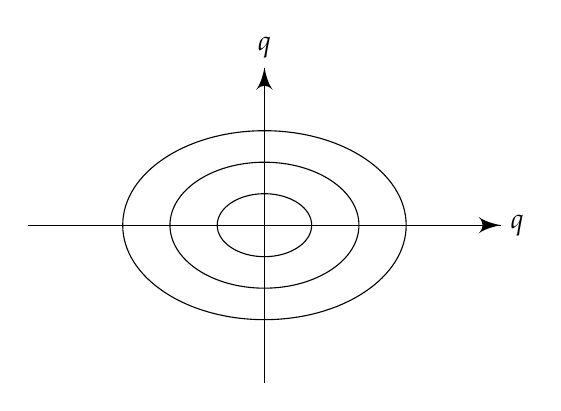
\begin{tikzpicture}
      \draw [->] (-3, 0) -- (3, 0) node [right] {$q$};
      \draw [->] (0, -2) -- (0, 2) node [above] {$q$};

      \foreach \x in {0.4, 0.8, 1.2} {
        \begin{scope}[scale=\x]
          \draw ellipse (1.5 and 1);
        \end{scope}
      }
    \end{tikzpicture}
  \end{center}
  We note that the ellipses are each homeomorphic to $S^1$. Now we introduce the coordinate transformation $(q, p) \mapsto (\phi, I)$, defined by
  \[
    q = \sqrt{\frac{2I}{\omega}} \sin \phi,\quad p = \sqrt{2I\omega} \cos \phi,
  \]
Hence, $\phi$ is the angle coordinate that parametrizes $S^1$ in the Arnold-Liouville theorem.

  We can manually show that this transformation is canonical, but it is merely a computation and we will not waste time doing that. In these new coordinates, the Hamiltonian looks like
  \[
    \tilde{H}(\phi, I) = H(q(\phi, I), p(\phi, I)) = \omega I.
  \]
The Hamiltonian is independent of $\phi$! Therefore, the Hamilton equations become
  \[
    \dot\phi = \frac{\partial \tilde{H}}{ \partial I} = \omega,\quad \dot{I} = -\frac{\partial \tilde{H}}{\partial \phi} = 0.
  \]
  We can integrate up to obtain
  \[
    \phi(t) = \phi_0 + \omega t,\quad I(t) = I_0.
  \]
It is interesting to consider the integral along paths of constant $H$:
  \begin{align*}
    \frac{1}{2\pi}\oint p \;\d q &= \frac{1}{2\pi} \int_0^{2\pi}p(\phi, I) \left(\frac{\partial q}{\partial \phi} \;\d \phi + \frac{\partial q}{\partial I} \;\d I\right)\\
    &= \frac{1}{2\pi} \int_0^{2\pi}p(\phi, I) \left(\frac{\partial q}{\partial \phi} \;\d \phi\right)\\
    &= \frac{1}{2\pi} \int_0^{2\pi} \sqrt{\frac{2I}{\omega}}\sqrt{2I\omega} \cos^2 \phi \;\d \phi\\
    &= I~.
  \end{align*}
We could always have performed the integral $\frac{1}{2\pi} \oint p \;\d q$ along paths of constant $H$ without knowing anything about $I$ and $\phi$, and this would have magically gave us the new coordinate $I$. That's why it is called \term{integrable system}.
\end{example}











\begin{thebibliography}{99}

\bibitem{Nakahara}
Mikio, Nakahara. {\it Geometry, topology and physics}. CRC Press, 2003.

\bibitem{Morita}
Shigeyuki, Morita. {\it Geometry of differential forms}. Vol. 201. American Mathematical Soc., 2001.

\bibitem{Weinberg}
Steven. Weinberg, \textit{The first three minutes: a modern view of the origin of the universe}, Basic Books, 1993.


\bibitem{Witten:1982fp}
E.~Witten, {\it An SU(2) Anomaly}, Phys.Lett. \textbf{B117} (1982) 324-328


\bibitem{Hatcher}
A.~Hatcher, {\it Algebraic Topology}, \url{https://www.math.cornell.edu/~hatcher/AT/AT.pdf}


\bibitem{EGH}
T. Eguchi, P. B. Gilkey, and A J. Hanson. {\it Gravitation, gauge theories and differential geometry}. Physics reports 66, no. 6 (1980): 213-393.


\bibitem{Schwarz:1978}
Albert S. Schwarz,  \emph{The partition function of degenerate quadratic functional and Ray-Singer invariants}, Letters in Mathematical Physics 2.3 (1978): 247-252.

\bibitem{Witten:1988hf}
E.~Witten, {\it {Quantum Field Theory and the Jones Polynomial}},  {\em Commun.
  Math. Phys.} {\bf 121} (1989) 351--399.


\bibitem{index-book}
Shing-Tung Yau, ed. (2009), \textit{The Founders of Index Theory (2nd ed.)}, Somerville, Mass.: International Press of Boston, ISBN 978-1571461377 - Personal accounts on Atiyah, Bott, Hirzebruch and Singer.


\bibitem{Dai}
Xianzhe Dai, \textit{Lectures on Dirac Operators and Index Theory},

 \href{http://web.math.ucsb.edu/~dai/book.pdf}{ http://web.math.ucsb.edu/dai/book.pdf}

\bibitem{BGV}
Berline Getzler Vergne, \textit{Heat kernels and Dirac operators}, Springer Science \& Business Media, 2003.

\bibitem{Witten:1982}
E.~Witten, \textit{Supersymmetry and Morse theory}, J. diff. geom \textrm{17}.4 (1982): 661-692.


\bibitem{Witten:2005}

E.~Witten, \href{https://www.fields.utoronto.ca/audio/04-05/distinguished_lectures/witten3/}{2004-2005 Distinguished Lecture Series  at the Fields Institute.}

\bibitem{Witten:2015}
E.~Witten, \textit{Three Lectures On Topological Phases Of Matter} \href{http://arxiv.org/abs/1510.07698}{[arXiv:1510.07698]}.


\bibitem{Candelas}
P. Candelas, X. C. de La Ossa, P. S. Green, L. Parkes, \textit{A pair of Calabi-Yau manifolds as an exactly soluble superconformal theory}. Nucl.Phys. B359 (1991) 21-74.

\bibitem{Bouchard}
Vincent. Bouchard,  \textit{Lectures on complex geometry, Calabi-Yau manifolds and toric geometry.} \href{http://arxiv.org/abs/hep-th/0702063}{hep-th/0702063} (2007).

\bibitem{Calabi-Yau}
Calabi-Yau manifolds, 
\url{http://www.scholarpedia.org/article/Calabi-Yau_manifold}

\end{thebibliography}

\end{document}
